%
% header.tex
%
\documentclass[%
	pdftex,%              PDFTex verwenden
	a4paper,%             A4 Papier
	twoside,%             Einseitig
	bibtotoc,%    Literaturverzeichnis nummeriert einf�gen
	idxtotoc,%            Index ins Verzeichnis einf�gen
	halfparskip,%         Europ�ischer Satz mit abstand zwischen Abs�tzen
	chapterprefix,%       Kapitel anschreiben als Kapitel
	headsepline,%         Linie nach Kopfzeile
	%footsepline,%         Linie vor Fusszeile
	12pt,%                 Gr�ssere Schrift, besser lesbar am bildschrim
	openright,
	pointlessnumbers
]{scrbook}

\usepackage{scrpage2}

\usepackage{textcomp}

\newcommand{\xirp}{$\chi$irp\index{xirp@$\chi$irp}}
\newcommand{\xirpname}{\enquote{eXtendable interface for robotic purposes}}
\newcommand{\version}{2.4.0}
\newcommand{\devguideurl}{http://developer.berlios.de/docman/display_doc.php?docid=1711&group_id=8442}
\newcommand{\devguideurlname}{xirp.berlios.de}
\newcommand{\seegls}[1]{\textuparrow{#1}}

\usepackage{scrpage2}

% \renewcommand{\partformat}{\partname~\thepart}
% \renewcommand{\chapterformat}{\chapapp~\thechapter}
% \renewcommand{\othersectionlevelsformat}[1]{\csname the#1\endcsname\enskip}
% 
% \renewcommand{\partmarkformat}{\thepart\enskip}
% \renewcommand{\chaptermarkformat}{\chapapp~\thechapter\enskip}
% \renewcommand{\sectionmarkformat}{\thesection\enskip}
% \renewcommand{\subsectionmarkformat}{\thesubsection\enskip}
% \renewcommand{\subsubsectionmarkformat}{\thesubsubsection\enskip}
% \renewcommand{\paragraphmarkformat}{\theparagraph\enskip}
% \renewcommand{\subparagraphmarkformat}{\thesubparagraphmarkformat\enskip}

\renewcommand{\chaptermark}[1]{\markboth{\chaptermarkformat{#1}}{\chaptermarkformat{#1}}}

\renewcommand{\chapterpagestyle}{scrheadings}
\renewcommand{\indexpagestyle}{scrheadings}

% kopf und fusszeilen
\pagestyle{scrheadings}

\clearscrheadfoot
\rohead[\headmark~\pagemark]{\headmark~\pagemark}
\lehead[\pagemark~\headmark]{\pagemark~\headmark}
\setheadtopline{.4pt}
\setheadsepline{.4pt}

\setcounter{secnumdepth}{5}
\setcounter{tocdepth}{5}

% Paket f�r die Indexerstellung.
\usepackage{makeidx}
%Formattierungen f�r Indexfile
%Erste Ebene
\newcommand*{\indexdelim}{\ \hspace{0pt plus 1fil}\penalty0\null\nobreak
  \dotfill~}
%Zweite Ebene
\newcommand*{\indexdelimi}{~\dotfill\penalty0\ }
%Dritte Ebene
\newcommand*{\indexdelimii}{~\dotfill\penalty0\ }

%Abschnitts�berschrift
\newcommand*{\indexsection}[1]{%
  \ifx\empty#1\empty\else
  \hspace{0pt plus 2fil}{{\usekomafont{sectioning} #1}}\hspace{0pt plus
    1fil}\nopagebreak
  \fi
}
% Paket f�r �bersetzungen ins Deutsche
\usepackage[french,ngerman]{babel}

% Pakete um Latin1 Zeichnens�tze verwenden zu k�nnen und die dazu
% passenden Schriften.
\usepackage[latin1]{inputenc}
\usepackage[T1]{fontenc}

% Paket f�r Quotes
\usepackage[babel,french=guillemets,german=swiss]{csquotes}

% Paket um die Symbole des TS1 Zeichensatzes verwenden zu k�nnen.
%\usepackage{textcomp}

% Paket zum Erweitern der Tabelleneigenschaften
\usepackage{array}

% Paket um Grafiken einbetten zu k�nnen
\usepackage[pdftex]{graphicx}

% Spezielle Schrift verwenden.
%\usepackage{goudysans}

% Spezielle Schrift im Koma-Script setzen.
%\setkomafont{sectioning}{\normalfont\bfseries}
%\setkomafont{captionlabel}{\normalfont\bfseries}
%\setkomafont{pagehead}{\normalfont\itshape}
%\setkomafont{descriptionlabel}{\normalfont\bfseries}

% Zeilenumbruch bei Bildbeschreibungen.
\setcapindent{1em}

% mathematische symbole aus dem AMS Paket.
%\usepackage{amsmath}
%\usepackage{amssymb}

% Type 1 Fonts f�r bessere darstellung in PDF verwenden.
%\usepackage{mathptmx}           % Times + passende Mathefonts
%\usepackage[scaled=.92]{helvet} % skalierte Helvetica als \sfdefault
%\usepackage{courier}            % Courier als \ttdefault

% Paket um Textteile drehen zu k�nnen
\usepackage{rotating}

% Package f�r Farben im PDF
\usepackage{color}
\definecolor{AliceBlue}{rgb}{0.94,0.97,1.00}
\definecolor{AntiqueWhite1}{rgb}{1.00,0.94,0.86}
\definecolor{AntiqueWhite2}{rgb}{0.93,0.87,0.80}
\definecolor{AntiqueWhite3}{rgb}{0.80,0.75,0.69}
\definecolor{AntiqueWhite4}{rgb}{0.55,0.51,0.47}
\definecolor{AntiqueWhite}{rgb}{0.98,0.92,0.84}
\definecolor{BlanchedAlmond}{rgb}{1.00,0.92,0.80}
\definecolor{BlueViolet}{rgb}{0.54,0.17,0.89}
\definecolor{CadetBlue1}{rgb}{0.60,0.96,1.00}
\definecolor{CadetBlue2}{rgb}{0.56,0.90,0.93}
\definecolor{CadetBlue3}{rgb}{0.48,0.77,0.80}
\definecolor{CadetBlue4}{rgb}{0.33,0.53,0.55}
\definecolor{CadetBlue}{rgb}{0.37,0.62,0.63}
\definecolor{CornflowerBlue}{rgb}{0.39,0.58,0.93}
\definecolor{DarkBlue}{rgb}{0.00,0.00,0.55}
\definecolor{DarkCyan}{rgb}{0.00,0.55,0.55}
\definecolor{DarkGoldenrod1}{rgb}{1.00,0.73,0.06}
\definecolor{DarkGoldenrod2}{rgb}{0.93,0.68,0.05}
\definecolor{DarkGoldenrod3}{rgb}{0.80,0.58,0.05}
\definecolor{DarkGoldenrod4}{rgb}{0.55,0.40,0.03}
\definecolor{DarkGoldenrod}{rgb}{0.72,0.53,0.04}
\definecolor{DarkGray}{rgb}{0.66,0.66,0.66}
\definecolor{DarkGreen}{rgb}{0.00,0.39,0.00}
\definecolor{DarkGrey}{rgb}{0.66,0.66,0.66}
\definecolor{DarkKhaki}{rgb}{0.74,0.72,0.42}
\definecolor{DarkMagenta}{rgb}{0.55,0.00,0.55}
\definecolor{DarkOliveGreen1}{rgb}{0.79,1.00,0.44}
\definecolor{DarkOliveGreen2}{rgb}{0.74,0.93,0.41}
\definecolor{DarkOliveGreen3}{rgb}{0.64,0.80,0.35}
\definecolor{DarkOliveGreen4}{rgb}{0.43,0.55,0.24}
\definecolor{DarkOliveGreen}{rgb}{0.33,0.42,0.18}
\definecolor{DarkOrange1}{rgb}{1.00,0.50,0.00}
\definecolor{DarkOrange2}{rgb}{0.93,0.46,0.00}
\definecolor{DarkOrange3}{rgb}{0.80,0.40,0.00}
\definecolor{DarkOrange4}{rgb}{0.55,0.27,0.00}
\definecolor{DarkOrange}{rgb}{1.00,0.55,0.00}
\definecolor{DarkOrchid1}{rgb}{0.75,0.24,1.00}
\definecolor{DarkOrchid2}{rgb}{0.70,0.23,0.93}
\definecolor{DarkOrchid3}{rgb}{0.60,0.20,0.80}
\definecolor{DarkOrchid4}{rgb}{0.41,0.13,0.55}
\definecolor{DarkOrchid}{rgb}{0.60,0.20,0.80}
\definecolor{DarkRed}{rgb}{0.55,0.00,0.00}
\definecolor{DarkSalmon}{rgb}{0.91,0.59,0.48}
\definecolor{DarkSeaGreen1}{rgb}{0.76,1.00,0.76}
\definecolor{DarkSeaGreen2}{rgb}{0.71,0.93,0.71}
\definecolor{DarkSeaGreen3}{rgb}{0.61,0.80,0.61}
\definecolor{DarkSeaGreen4}{rgb}{0.41,0.55,0.41}
\definecolor{DarkSeaGreen}{rgb}{0.56,0.74,0.56}
\definecolor{DarkSlateBlue}{rgb}{0.28,0.24,0.55}
\definecolor{DarkSlateGray1}{rgb}{0.59,1.00,1.00}
\definecolor{DarkSlateGray2}{rgb}{0.55,0.93,0.93}
\definecolor{DarkSlateGray3}{rgb}{0.47,0.80,0.80}
\definecolor{DarkSlateGray4}{rgb}{0.32,0.55,0.55}
\definecolor{DarkSlateGray}{rgb}{0.18,0.31,0.31}
\definecolor{DarkSlateGrey}{rgb}{0.18,0.31,0.31}
\definecolor{DarkTurquoise}{rgb}{0.00,0.81,0.82}
\definecolor{DarkViolet}{rgb}{0.58,0.00,0.83}
\definecolor{DeepPink1}{rgb}{1.00,0.08,0.58}
\definecolor{DeepPink2}{rgb}{0.93,0.07,0.54}
\definecolor{DeepPink3}{rgb}{0.80,0.06,0.46}
\definecolor{DeepPink4}{rgb}{0.55,0.04,0.31}
\definecolor{DeepPink}{rgb}{1.00,0.08,0.58}
\definecolor{DeepSkyBlue1}{rgb}{0.00,0.75,1.00}
\definecolor{DeepSkyBlue2}{rgb}{0.00,0.70,0.93}
\definecolor{DeepSkyBlue3}{rgb}{0.00,0.60,0.80}
\definecolor{DeepSkyBlue4}{rgb}{0.00,0.41,0.55}
\definecolor{DeepSkyBlue}{rgb}{0.00,0.75,1.00}
\definecolor{DimGray}{rgb}{0.41,0.41,0.41}
\definecolor{DimGrey}{rgb}{0.41,0.41,0.41}
\definecolor{DodgerBlue1}{rgb}{0.12,0.56,1.00}
\definecolor{DodgerBlue2}{rgb}{0.11,0.53,0.93}
\definecolor{DodgerBlue3}{rgb}{0.09,0.45,0.80}
\definecolor{DodgerBlue4}{rgb}{0.06,0.31,0.55}
\definecolor{DodgerBlue}{rgb}{0.12,0.56,1.00}
\definecolor{FloralWhite}{rgb}{1.00,0.98,0.94}
\definecolor{ForestGreen}{rgb}{0.13,0.55,0.13}
\definecolor{GhostWhite}{rgb}{0.97,0.97,1.00}
\definecolor{GreenYellow}{rgb}{0.68,1.00,0.18}
\definecolor{HotPink1}{rgb}{1.00,0.43,0.71}
\definecolor{HotPink2}{rgb}{0.93,0.42,0.65}
\definecolor{HotPink3}{rgb}{0.80,0.38,0.56}
\definecolor{HotPink4}{rgb}{0.55,0.23,0.38}
\definecolor{HotPink}{rgb}{1.00,0.41,0.71}
\definecolor{IndianRed1}{rgb}{1.00,0.42,0.42}
\definecolor{IndianRed2}{rgb}{0.93,0.39,0.39}
\definecolor{IndianRed3}{rgb}{0.80,0.33,0.33}
\definecolor{IndianRed4}{rgb}{0.55,0.23,0.23}
\definecolor{IndianRed}{rgb}{0.80,0.36,0.36}
\definecolor{LavenderBlush1}{rgb}{1.00,0.94,0.96}
\definecolor{LavenderBlush2}{rgb}{0.93,0.88,0.90}
\definecolor{LavenderBlush3}{rgb}{0.80,0.76,0.77}
\definecolor{LavenderBlush4}{rgb}{0.55,0.51,0.53}
\definecolor{LavenderBlush}{rgb}{1.00,0.94,0.96}
\definecolor{LawnGreen}{rgb}{0.49,0.99,0.00}
\definecolor{LemonChiffon1}{rgb}{1.00,0.98,0.80}
\definecolor{LemonChiffon2}{rgb}{0.93,0.91,0.75}
\definecolor{LemonChiffon3}{rgb}{0.80,0.79,0.65}
\definecolor{LemonChiffon4}{rgb}{0.55,0.54,0.44}
\definecolor{LemonChiffon}{rgb}{1.00,0.98,0.80}
\definecolor{LightBlue1}{rgb}{0.75,0.94,1.00}
\definecolor{LightBlue2}{rgb}{0.70,0.87,0.93}
\definecolor{LightBlue3}{rgb}{0.60,0.75,0.80}
\definecolor{LightBlue4}{rgb}{0.41,0.51,0.55}
\definecolor{LightBlue}{rgb}{0.68,0.85,0.90}
\definecolor{LightCoral}{rgb}{0.94,0.50,0.50}
\definecolor{LightCyan1}{rgb}{0.88,1.00,1.00}
\definecolor{LightCyan2}{rgb}{0.82,0.93,0.93}
\definecolor{LightCyan3}{rgb}{0.71,0.80,0.80}
\definecolor{LightCyan4}{rgb}{0.48,0.55,0.55}
\definecolor{LightCyan}{rgb}{0.88,1.00,1.00}
\definecolor{LightGoldenrod1}{rgb}{1.00,0.93,0.55}
\definecolor{LightGoldenrod2}{rgb}{0.93,0.86,0.51}
\definecolor{LightGoldenrod3}{rgb}{0.80,0.75,0.44}
\definecolor{LightGoldenrod4}{rgb}{0.55,0.51,0.30}
\definecolor{LightGoldenrodYellow}{rgb}{0.98,0.98,0.82}
\definecolor{LightGoldenrod}{rgb}{0.93,0.87,0.51}
\definecolor{LightGray}{rgb}{0.83,0.83,0.83}
\definecolor{LightGreen}{rgb}{0.56,0.93,0.56}
\definecolor{LightGrey}{rgb}{0.83,0.83,0.83}
\definecolor{LightPink1}{rgb}{1.00,0.68,0.73}
\definecolor{LightPink2}{rgb}{0.93,0.64,0.68}
\definecolor{LightPink3}{rgb}{0.80,0.55,0.58}
\definecolor{LightPink4}{rgb}{0.55,0.37,0.40}
\definecolor{LightPink}{rgb}{1.00,0.71,0.76}
\definecolor{LightSalmon1}{rgb}{1.00,0.63,0.48}
\definecolor{LightSalmon2}{rgb}{0.93,0.58,0.45}
\definecolor{LightSalmon3}{rgb}{0.80,0.51,0.38}
\definecolor{LightSalmon4}{rgb}{0.55,0.34,0.26}
\definecolor{LightSalmon}{rgb}{1.00,0.63,0.48}
\definecolor{LightSeaGreen}{rgb}{0.13,0.70,0.67}
\definecolor{LightSkyBlue1}{rgb}{0.69,0.89,1.00}
\definecolor{LightSkyBlue2}{rgb}{0.64,0.83,0.93}
\definecolor{LightSkyBlue3}{rgb}{0.55,0.71,0.80}
\definecolor{LightSkyBlue4}{rgb}{0.38,0.48,0.55}
\definecolor{LightSkyBlue}{rgb}{0.53,0.81,0.98}
\definecolor{LightSlateBlue}{rgb}{0.52,0.44,1.00}
\definecolor{LightSlateGray}{rgb}{0.47,0.53,0.60}
\definecolor{LightSlateGrey}{rgb}{0.47,0.53,0.60}
\definecolor{LightSteelBlue1}{rgb}{0.79,0.88,1.00}
\definecolor{LightSteelBlue2}{rgb}{0.74,0.82,0.93}
\definecolor{LightSteelBlue3}{rgb}{0.64,0.71,0.80}
\definecolor{LightSteelBlue4}{rgb}{0.43,0.48,0.55}
\definecolor{LightSteelBlue}{rgb}{0.69,0.77,0.87}
\definecolor{LightYellow1}{rgb}{1.00,1.00,0.88}
\definecolor{LightYellow2}{rgb}{0.93,0.93,0.82}
\definecolor{LightYellow3}{rgb}{0.80,0.80,0.71}
\definecolor{LightYellow4}{rgb}{0.55,0.55,0.48}
\definecolor{LightYellow}{rgb}{1.00,1.00,0.88}
\definecolor{LimeGreen}{rgb}{0.20,0.80,0.20}
\definecolor{MediumAquamarine}{rgb}{0.40,0.80,0.67}
\definecolor{MediumBlue}{rgb}{0.00,0.00,0.80}
\definecolor{MediumOrchid1}{rgb}{0.88,0.40,1.00}
\definecolor{MediumOrchid2}{rgb}{0.82,0.37,0.93}
\definecolor{MediumOrchid3}{rgb}{0.71,0.32,0.80}
\definecolor{MediumOrchid4}{rgb}{0.48,0.22,0.55}
\definecolor{MediumOrchid}{rgb}{0.73,0.33,0.83}
\definecolor{MediumPurple1}{rgb}{0.67,0.51,1.00}
\definecolor{MediumPurple2}{rgb}{0.62,0.47,0.93}
\definecolor{MediumPurple3}{rgb}{0.54,0.41,0.80}
\definecolor{MediumPurple4}{rgb}{0.36,0.28,0.55}
\definecolor{MediumPurple}{rgb}{0.58,0.44,0.86}
\definecolor{MediumSeaGreen}{rgb}{0.24,0.70,0.44}
\definecolor{MediumSlateBlue}{rgb}{0.48,0.41,0.93}
\definecolor{MediumSpringGreen}{rgb}{0.00,0.98,0.60}
\definecolor{MediumTurquoise}{rgb}{0.28,0.82,0.80}
\definecolor{MediumVioletRed}{rgb}{0.78,0.08,0.52}
\definecolor{MidnightBlue}{rgb}{0.10,0.10,0.44}
\definecolor{MintCream}{rgb}{0.96,1.00,0.98}
\definecolor{MistyRose1}{rgb}{1.00,0.89,0.88}
\definecolor{MistyRose2}{rgb}{0.93,0.84,0.82}
\definecolor{MistyRose3}{rgb}{0.80,0.72,0.71}
\definecolor{MistyRose4}{rgb}{0.55,0.49,0.48}
\definecolor{MistyRose}{rgb}{1.00,0.89,0.88}
\definecolor{NavajoWhite1}{rgb}{1.00,0.87,0.68}
\definecolor{NavajoWhite2}{rgb}{0.93,0.81,0.63}
\definecolor{NavajoWhite3}{rgb}{0.80,0.70,0.55}
\definecolor{NavajoWhite4}{rgb}{0.55,0.47,0.37}
\definecolor{NavajoWhite}{rgb}{1.00,0.87,0.68}
\definecolor{NavyBlue}{rgb}{0.00,0.00,0.50}
\definecolor{OldLace}{rgb}{0.99,0.96,0.90}
\definecolor{OliveDrab1}{rgb}{0.75,1.00,0.24}
\definecolor{OliveDrab2}{rgb}{0.70,0.93,0.23}
\definecolor{OliveDrab3}{rgb}{0.60,0.80,0.20}
\definecolor{OliveDrab4}{rgb}{0.41,0.55,0.13}
\definecolor{OliveDrab}{rgb}{0.42,0.56,0.14}
\definecolor{OrangeRed1}{rgb}{1.00,0.27,0.00}
\definecolor{OrangeRed2}{rgb}{0.93,0.25,0.00}
\definecolor{OrangeRed3}{rgb}{0.80,0.22,0.00}
\definecolor{OrangeRed4}{rgb}{0.55,0.15,0.00}
\definecolor{OrangeRed}{rgb}{1.00,0.27,0.00}
\definecolor{PaleGoldenrod}{rgb}{0.93,0.91,0.67}
\definecolor{PaleGreen1}{rgb}{0.60,1.00,0.60}
\definecolor{PaleGreen2}{rgb}{0.56,0.93,0.56}
\definecolor{PaleGreen3}{rgb}{0.49,0.80,0.49}
\definecolor{PaleGreen4}{rgb}{0.33,0.55,0.33}
\definecolor{PaleGreen}{rgb}{0.60,0.98,0.60}
\definecolor{PaleTurquoise1}{rgb}{0.73,1.00,1.00}
\definecolor{PaleTurquoise2}{rgb}{0.68,0.93,0.93}
\definecolor{PaleTurquoise3}{rgb}{0.59,0.80,0.80}
\definecolor{PaleTurquoise4}{rgb}{0.40,0.55,0.55}
\definecolor{PaleTurquoise}{rgb}{0.69,0.93,0.93}
\definecolor{PaleVioletRed1}{rgb}{1.00,0.51,0.67}
\definecolor{PaleVioletRed2}{rgb}{0.93,0.47,0.62}
\definecolor{PaleVioletRed3}{rgb}{0.80,0.41,0.54}
\definecolor{PaleVioletRed4}{rgb}{0.55,0.28,0.36}
\definecolor{PaleVioletRed}{rgb}{0.86,0.44,0.58}
\definecolor{PapayaWhip}{rgb}{1.00,0.94,0.84}
\definecolor{PeachPuff1}{rgb}{1.00,0.85,0.73}
\definecolor{PeachPuff2}{rgb}{0.93,0.80,0.68}
\definecolor{PeachPuff3}{rgb}{0.80,0.69,0.58}
\definecolor{PeachPuff4}{rgb}{0.55,0.47,0.40}
\definecolor{PeachPuff}{rgb}{1.00,0.85,0.73}
\definecolor{PowderBlue}{rgb}{0.69,0.88,0.90}
\definecolor{RosyBrown1}{rgb}{1.00,0.76,0.76}
\definecolor{RosyBrown2}{rgb}{0.93,0.71,0.71}
\definecolor{RosyBrown3}{rgb}{0.80,0.61,0.61}
\definecolor{RosyBrown4}{rgb}{0.55,0.41,0.41}
\definecolor{RosyBrown}{rgb}{0.74,0.56,0.56}
\definecolor{RoyalBlue1}{rgb}{0.28,0.46,1.00}
\definecolor{RoyalBlue2}{rgb}{0.26,0.43,0.93}
\definecolor{RoyalBlue3}{rgb}{0.23,0.37,0.80}
\definecolor{RoyalBlue4}{rgb}{0.15,0.25,0.55}
\definecolor{RoyalBlue}{rgb}{0.25,0.41,0.88}
\definecolor{SaddleBrown}{rgb}{0.55,0.27,0.07}
\definecolor{SandyBrown}{rgb}{0.96,0.64,0.38}
\definecolor{SeaGreen1}{rgb}{0.33,1.00,0.62}
\definecolor{SeaGreen2}{rgb}{0.31,0.93,0.58}
\definecolor{SeaGreen3}{rgb}{0.26,0.80,0.50}
\definecolor{SeaGreen4}{rgb}{0.18,0.55,0.34}
\definecolor{SeaGreen}{rgb}{0.18,0.55,0.34}
\definecolor{SkyBlue1}{rgb}{0.53,0.81,1.00}
\definecolor{SkyBlue2}{rgb}{0.49,0.75,0.93}
\definecolor{SkyBlue3}{rgb}{0.42,0.65,0.80}
\definecolor{SkyBlue4}{rgb}{0.29,0.44,0.55}
\definecolor{SkyBlue}{rgb}{0.53,0.81,0.92}
\definecolor{SlateBlue1}{rgb}{0.51,0.44,1.00}
\definecolor{SlateBlue2}{rgb}{0.48,0.40,0.93}
\definecolor{SlateBlue3}{rgb}{0.41,0.35,0.80}
\definecolor{SlateBlue4}{rgb}{0.28,0.24,0.55}
\definecolor{SlateBlue}{rgb}{0.42,0.35,0.80}
\definecolor{SlateGray1}{rgb}{0.78,0.89,1.00}
\definecolor{SlateGray2}{rgb}{0.73,0.83,0.93}
\definecolor{SlateGray3}{rgb}{0.62,0.71,0.80}
\definecolor{SlateGray4}{rgb}{0.42,0.48,0.55}
\definecolor{SlateGray}{rgb}{0.44,0.50,0.56}
\definecolor{SlateGrey}{rgb}{0.44,0.50,0.56}
\definecolor{SpringGreen1}{rgb}{0.00,1.00,0.50}
\definecolor{SpringGreen2}{rgb}{0.00,0.93,0.46}
\definecolor{SpringGreen3}{rgb}{0.00,0.80,0.40}
\definecolor{SpringGreen4}{rgb}{0.00,0.55,0.27}
\definecolor{SpringGreen}{rgb}{0.00,1.00,0.50}
\definecolor{SteelBlue1}{rgb}{0.39,0.72,1.00}
\definecolor{SteelBlue2}{rgb}{0.36,0.67,0.93}
\definecolor{SteelBlue3}{rgb}{0.31,0.58,0.80}
\definecolor{SteelBlue4}{rgb}{0.21,0.39,0.55}
\definecolor{SteelBlue}{rgb}{0.27,0.51,0.71}
\definecolor{VioletRed1}{rgb}{1.00,0.24,0.59}
\definecolor{VioletRed2}{rgb}{0.93,0.23,0.55}
\definecolor{VioletRed3}{rgb}{0.80,0.20,0.47}
\definecolor{VioletRed4}{rgb}{0.55,0.13,0.32}
\definecolor{VioletRed}{rgb}{0.82,0.13,0.56}
\definecolor{WhiteSmoke}{rgb}{0.96,0.96,0.96}
\definecolor{YellowGreen}{rgb}{0.60,0.80,0.20}
\definecolor{aliceblue}{rgb}{0.94,0.97,1.00}
\definecolor{antiquewhite}{rgb}{0.98,0.92,0.84}
\definecolor{aquamarine1}{rgb}{0.50,1.00,0.83}
\definecolor{aquamarine2}{rgb}{0.46,0.93,0.78}
\definecolor{aquamarine3}{rgb}{0.40,0.80,0.67}
\definecolor{aquamarine4}{rgb}{0.27,0.55,0.45}
\definecolor{aquamarine}{rgb}{0.50,1.00,0.83}
\definecolor{azure1}{rgb}{0.94,1.00,1.00}
\definecolor{azure2}{rgb}{0.88,0.93,0.93}
\definecolor{azure3}{rgb}{0.76,0.80,0.80}
\definecolor{azure4}{rgb}{0.51,0.55,0.55}
\definecolor{azure}{rgb}{0.94,1.00,1.00}
\definecolor{beige}{rgb}{0.96,0.96,0.86}
\definecolor{bisque1}{rgb}{1.00,0.89,0.77}
\definecolor{bisque2}{rgb}{0.93,0.84,0.72}
\definecolor{bisque3}{rgb}{0.80,0.72,0.62}
\definecolor{bisque4}{rgb}{0.55,0.49,0.42}
\definecolor{bisque}{rgb}{1.00,0.89,0.77}
\definecolor{black}{rgb}{0.00,0.00,0.00}
\definecolor{blanchedalmond}{rgb}{1.00,0.92,0.80}
\definecolor{blue1}{rgb}{0.00,0.00,1.00}
\definecolor{blue2}{rgb}{0.00,0.00,0.93}
\definecolor{blue3}{rgb}{0.00,0.00,0.80}
\definecolor{blue4}{rgb}{0.00,0.00,0.55}
\definecolor{blueviolet}{rgb}{0.54,0.17,0.89}
\definecolor{blue}{rgb}{0.00,0.00,1.00}
\definecolor{brown1}{rgb}{1.00,0.25,0.25}
\definecolor{brown2}{rgb}{0.93,0.23,0.23}
\definecolor{brown3}{rgb}{0.80,0.20,0.20}
\definecolor{brown4}{rgb}{0.55,0.14,0.14}
\definecolor{brown}{rgb}{0.65,0.16,0.16}
\definecolor{burlywood1}{rgb}{1.00,0.83,0.61}
\definecolor{burlywood2}{rgb}{0.93,0.77,0.57}
\definecolor{burlywood3}{rgb}{0.80,0.67,0.49}
\definecolor{burlywood4}{rgb}{0.55,0.45,0.33}
\definecolor{burlywood}{rgb}{0.87,0.72,0.53}
\definecolor{cadetblue}{rgb}{0.37,0.62,0.63}
\definecolor{chartreuse1}{rgb}{0.50,1.00,0.00}
\definecolor{chartreuse2}{rgb}{0.46,0.93,0.00}
\definecolor{chartreuse3}{rgb}{0.40,0.80,0.00}
\definecolor{chartreuse4}{rgb}{0.27,0.55,0.00}
\definecolor{chartreuse}{rgb}{0.50,1.00,0.00}
\definecolor{chocolate1}{rgb}{1.00,0.50,0.14}
\definecolor{chocolate2}{rgb}{0.93,0.46,0.13}
\definecolor{chocolate3}{rgb}{0.80,0.40,0.11}
\definecolor{chocolate4}{rgb}{0.55,0.27,0.07}
\definecolor{chocolate}{rgb}{0.82,0.41,0.12}
\definecolor{coral1}{rgb}{1.00,0.45,0.34}
\definecolor{coral2}{rgb}{0.93,0.42,0.31}
\definecolor{coral3}{rgb}{0.80,0.36,0.27}
\definecolor{coral4}{rgb}{0.55,0.24,0.18}
\definecolor{coral}{rgb}{1.00,0.50,0.31}
\definecolor{cornflowerblue}{rgb}{0.39,0.58,0.93}
\definecolor{cornsilk1}{rgb}{1.00,0.97,0.86}
\definecolor{cornsilk2}{rgb}{0.93,0.91,0.80}
\definecolor{cornsilk3}{rgb}{0.80,0.78,0.69}
\definecolor{cornsilk4}{rgb}{0.55,0.53,0.47}
\definecolor{cornsilk}{rgb}{1.00,0.97,0.86}
\definecolor{cyan1}{rgb}{0.00,1.00,1.00}
\definecolor{cyan2}{rgb}{0.00,0.93,0.93}
\definecolor{cyan3}{rgb}{0.00,0.80,0.80}
\definecolor{cyan4}{rgb}{0.00,0.55,0.55}
\definecolor{cyan}{rgb}{0.00,1.00,1.00}
\definecolor{darkblue}{rgb}{0.00,0.00,0.55}
\definecolor{darkcyan}{rgb}{0.00,0.55,0.55}
\definecolor{darkgoldenrod}{rgb}{0.72,0.53,0.04}
\definecolor{darkgray}{rgb}{0.66,0.66,0.66}
\definecolor{darkgreen}{rgb}{0.00,0.39,0.00}
\definecolor{darkgrey}{rgb}{0.66,0.66,0.66}
\definecolor{darkkhaki}{rgb}{0.74,0.72,0.42}
\definecolor{darkmagenta}{rgb}{0.55,0.00,0.55}
\definecolor{darkolive}{rgb}{0.33,0.42,0.18}
\definecolor{darkorange}{rgb}{1.00,0.55,0.00}
\definecolor{darkorchid}{rgb}{0.60,0.20,0.80}
\definecolor{darkred}{rgb}{0.55,0.00,0.00}
\definecolor{darksalmon}{rgb}{0.91,0.59,0.48}
\definecolor{darksea}{rgb}{0.56,0.74,0.56}
\definecolor{darkslate}{rgb}{0.18,0.31,0.31}
\definecolor{darkslate}{rgb}{0.18,0.31,0.31}
\definecolor{darkslate}{rgb}{0.28,0.24,0.55}
\definecolor{darkturquoise}{rgb}{0.00,0.81,0.82}
\definecolor{darkviolet}{rgb}{0.58,0.00,0.83}
\definecolor{deeppink}{rgb}{1.00,0.08,0.58}
\definecolor{deepsky}{rgb}{0.00,0.75,1.00}
\definecolor{dimgray}{rgb}{0.41,0.41,0.41}
\definecolor{dimgrey}{rgb}{0.41,0.41,0.41}
\definecolor{dodgerblue}{rgb}{0.12,0.56,1.00}
\definecolor{firebrick1}{rgb}{1.00,0.19,0.19}
\definecolor{firebrick2}{rgb}{0.93,0.17,0.17}
\definecolor{firebrick3}{rgb}{0.80,0.15,0.15}
\definecolor{firebrick4}{rgb}{0.55,0.10,0.10}
\definecolor{firebrick}{rgb}{0.70,0.13,0.13}
\definecolor{floralwhite}{rgb}{1.00,0.98,0.94}
\definecolor{forestgreen}{rgb}{0.13,0.55,0.13}
\definecolor{gainsboro}{rgb}{0.86,0.86,0.86}
\definecolor{ghostwhite}{rgb}{0.97,0.97,1.00}
\definecolor{gold1}{rgb}{1.00,0.84,0.00}
\definecolor{gold2}{rgb}{0.93,0.79,0.00}
\definecolor{gold3}{rgb}{0.80,0.68,0.00}
\definecolor{gold4}{rgb}{0.55,0.46,0.00}
\definecolor{goldenrod1}{rgb}{1.00,0.76,0.15}
\definecolor{goldenrod2}{rgb}{0.93,0.71,0.13}
\definecolor{goldenrod3}{rgb}{0.80,0.61,0.11}
\definecolor{goldenrod4}{rgb}{0.55,0.41,0.08}
\definecolor{goldenrod}{rgb}{0.85,0.65,0.13}
\definecolor{gold}{rgb}{1.00,0.84,0.00}
\definecolor{gray0}{rgb}{0.00,0.00,0.00}
\definecolor{gray100}{rgb}{1.00,1.00,1.00}
\definecolor{gray10}{rgb}{0.10,0.10,0.10}
\definecolor{gray11}{rgb}{0.11,0.11,0.11}
\definecolor{gray12}{rgb}{0.12,0.12,0.12}
\definecolor{gray13}{rgb}{0.13,0.13,0.13}
\definecolor{gray14}{rgb}{0.14,0.14,0.14}
\definecolor{gray15}{rgb}{0.15,0.15,0.15}
\definecolor{gray16}{rgb}{0.16,0.16,0.16}
\definecolor{gray17}{rgb}{0.17,0.17,0.17}
\definecolor{gray18}{rgb}{0.18,0.18,0.18}
\definecolor{gray19}{rgb}{0.19,0.19,0.19}
\definecolor{gray1}{rgb}{0.01,0.01,0.01}
\definecolor{gray20}{rgb}{0.20,0.20,0.20}
\definecolor{gray21}{rgb}{0.21,0.21,0.21}
\definecolor{gray22}{rgb}{0.22,0.22,0.22}
\definecolor{gray23}{rgb}{0.23,0.23,0.23}
\definecolor{gray24}{rgb}{0.24,0.24,0.24}
\definecolor{gray25}{rgb}{0.25,0.25,0.25}
\definecolor{gray26}{rgb}{0.26,0.26,0.26}
\definecolor{gray27}{rgb}{0.27,0.27,0.27}
\definecolor{gray28}{rgb}{0.28,0.28,0.28}
\definecolor{gray29}{rgb}{0.29,0.29,0.29}
\definecolor{gray2}{rgb}{0.02,0.02,0.02}
\definecolor{gray30}{rgb}{0.30,0.30,0.30}
\definecolor{gray31}{rgb}{0.31,0.31,0.31}
\definecolor{gray32}{rgb}{0.32,0.32,0.32}
\definecolor{gray33}{rgb}{0.33,0.33,0.33}
\definecolor{gray34}{rgb}{0.34,0.34,0.34}
\definecolor{gray35}{rgb}{0.35,0.35,0.35}
\definecolor{gray36}{rgb}{0.36,0.36,0.36}
\definecolor{gray37}{rgb}{0.37,0.37,0.37}
\definecolor{gray38}{rgb}{0.38,0.38,0.38}
\definecolor{gray39}{rgb}{0.39,0.39,0.39}
\definecolor{gray3}{rgb}{0.03,0.03,0.03}
\definecolor{gray40}{rgb}{0.40,0.40,0.40}
\definecolor{gray41}{rgb}{0.41,0.41,0.41}
\definecolor{gray42}{rgb}{0.42,0.42,0.42}
\definecolor{gray43}{rgb}{0.43,0.43,0.43}
\definecolor{gray44}{rgb}{0.44,0.44,0.44}
\definecolor{gray45}{rgb}{0.45,0.45,0.45}
\definecolor{gray46}{rgb}{0.46,0.46,0.46}
\definecolor{gray47}{rgb}{0.47,0.47,0.47}
\definecolor{gray48}{rgb}{0.48,0.48,0.48}
\definecolor{gray49}{rgb}{0.49,0.49,0.49}
\definecolor{gray4}{rgb}{0.04,0.04,0.04}
\definecolor{gray50}{rgb}{0.50,0.50,0.50}
\definecolor{gray51}{rgb}{0.51,0.51,0.51}
\definecolor{gray52}{rgb}{0.52,0.52,0.52}
\definecolor{gray53}{rgb}{0.53,0.53,0.53}
\definecolor{gray54}{rgb}{0.54,0.54,0.54}
\definecolor{gray55}{rgb}{0.55,0.55,0.55}
\definecolor{gray56}{rgb}{0.56,0.56,0.56}
\definecolor{gray57}{rgb}{0.57,0.57,0.57}
\definecolor{gray58}{rgb}{0.58,0.58,0.58}
\definecolor{gray59}{rgb}{0.59,0.59,0.59}
\definecolor{gray5}{rgb}{0.05,0.05,0.05}
\definecolor{gray60}{rgb}{0.60,0.60,0.60}
\definecolor{gray61}{rgb}{0.61,0.61,0.61}
\definecolor{gray62}{rgb}{0.62,0.62,0.62}
\definecolor{gray63}{rgb}{0.63,0.63,0.63}
\definecolor{gray64}{rgb}{0.64,0.64,0.64}
\definecolor{gray65}{rgb}{0.65,0.65,0.65}
\definecolor{gray66}{rgb}{0.66,0.66,0.66}
\definecolor{gray67}{rgb}{0.67,0.67,0.67}
\definecolor{gray68}{rgb}{0.68,0.68,0.68}
\definecolor{gray69}{rgb}{0.69,0.69,0.69}
\definecolor{gray6}{rgb}{0.06,0.06,0.06}
\definecolor{gray70}{rgb}{0.70,0.70,0.70}
\definecolor{gray71}{rgb}{0.71,0.71,0.71}
\definecolor{gray72}{rgb}{0.72,0.72,0.72}
\definecolor{gray73}{rgb}{0.73,0.73,0.73}
\definecolor{gray74}{rgb}{0.74,0.74,0.74}
\definecolor{gray75}{rgb}{0.75,0.75,0.75}
\definecolor{gray76}{rgb}{0.76,0.76,0.76}
\definecolor{gray77}{rgb}{0.77,0.77,0.77}
\definecolor{gray78}{rgb}{0.78,0.78,0.78}
\definecolor{gray79}{rgb}{0.79,0.79,0.79}
\definecolor{gray7}{rgb}{0.07,0.07,0.07}
\definecolor{gray80}{rgb}{0.80,0.80,0.80}
\definecolor{gray81}{rgb}{0.81,0.81,0.81}
\definecolor{gray82}{rgb}{0.82,0.82,0.82}
\definecolor{gray83}{rgb}{0.83,0.83,0.83}
\definecolor{gray84}{rgb}{0.84,0.84,0.84}
\definecolor{gray85}{rgb}{0.85,0.85,0.85}
\definecolor{gray86}{rgb}{0.86,0.86,0.86}
\definecolor{gray87}{rgb}{0.87,0.87,0.87}
\definecolor{gray88}{rgb}{0.88,0.88,0.88}
\definecolor{gray89}{rgb}{0.89,0.89,0.89}
\definecolor{gray8}{rgb}{0.08,0.08,0.08}
\definecolor{gray90}{rgb}{0.90,0.90,0.90}
\definecolor{gray91}{rgb}{0.91,0.91,0.91}
\definecolor{gray92}{rgb}{0.92,0.92,0.92}
\definecolor{gray93}{rgb}{0.93,0.93,0.93}
\definecolor{gray94}{rgb}{0.94,0.94,0.94}
\definecolor{gray95}{rgb}{0.95,0.95,0.95}
\definecolor{gray96}{rgb}{0.96,0.96,0.96}
\definecolor{gray97}{rgb}{0.97,0.97,0.97}
\definecolor{gray98}{rgb}{0.98,0.98,0.98}
\definecolor{gray99}{rgb}{0.99,0.99,0.99}
\definecolor{gray9}{rgb}{0.09,0.09,0.09}
\definecolor{gray}{rgb}{0.75,0.75,0.75}
\definecolor{green1}{rgb}{0.00,1.00,0.00}
\definecolor{green2}{rgb}{0.00,0.93,0.00}
\definecolor{green3}{rgb}{0.00,0.80,0.00}
\definecolor{green4}{rgb}{0.00,0.55,0.00}
\definecolor{greenyellow}{rgb}{0.68,1.00,0.18}
\definecolor{green}{rgb}{0.00,1.00,0.00}
\definecolor{grey0}{rgb}{0.00,0.00,0.00}
\definecolor{grey100}{rgb}{1.00,1.00,1.00}
\definecolor{grey10}{rgb}{0.10,0.10,0.10}
\definecolor{grey11}{rgb}{0.11,0.11,0.11}
\definecolor{grey12}{rgb}{0.12,0.12,0.12}
\definecolor{grey13}{rgb}{0.13,0.13,0.13}
\definecolor{grey14}{rgb}{0.14,0.14,0.14}
\definecolor{grey15}{rgb}{0.15,0.15,0.15}
\definecolor{grey16}{rgb}{0.16,0.16,0.16}
\definecolor{grey17}{rgb}{0.17,0.17,0.17}
\definecolor{grey18}{rgb}{0.18,0.18,0.18}
\definecolor{grey19}{rgb}{0.19,0.19,0.19}
\definecolor{grey1}{rgb}{0.01,0.01,0.01}
\definecolor{grey20}{rgb}{0.20,0.20,0.20}
\definecolor{grey21}{rgb}{0.21,0.21,0.21}
\definecolor{grey22}{rgb}{0.22,0.22,0.22}
\definecolor{grey23}{rgb}{0.23,0.23,0.23}
\definecolor{grey24}{rgb}{0.24,0.24,0.24}
\definecolor{grey25}{rgb}{0.25,0.25,0.25}
\definecolor{grey26}{rgb}{0.26,0.26,0.26}
\definecolor{grey27}{rgb}{0.27,0.27,0.27}
\definecolor{grey28}{rgb}{0.28,0.28,0.28}
\definecolor{grey29}{rgb}{0.29,0.29,0.29}
\definecolor{grey2}{rgb}{0.02,0.02,0.02}
\definecolor{grey30}{rgb}{0.30,0.30,0.30}
\definecolor{grey31}{rgb}{0.31,0.31,0.31}
\definecolor{grey32}{rgb}{0.32,0.32,0.32}
\definecolor{grey33}{rgb}{0.33,0.33,0.33}
\definecolor{grey34}{rgb}{0.34,0.34,0.34}
\definecolor{grey35}{rgb}{0.35,0.35,0.35}
\definecolor{grey36}{rgb}{0.36,0.36,0.36}
\definecolor{grey37}{rgb}{0.37,0.37,0.37}
\definecolor{grey38}{rgb}{0.38,0.38,0.38}
\definecolor{grey39}{rgb}{0.39,0.39,0.39}
\definecolor{grey3}{rgb}{0.03,0.03,0.03}
\definecolor{grey40}{rgb}{0.40,0.40,0.40}
\definecolor{grey41}{rgb}{0.41,0.41,0.41}
\definecolor{grey42}{rgb}{0.42,0.42,0.42}
\definecolor{grey43}{rgb}{0.43,0.43,0.43}
\definecolor{grey44}{rgb}{0.44,0.44,0.44}
\definecolor{grey45}{rgb}{0.45,0.45,0.45}
\definecolor{grey46}{rgb}{0.46,0.46,0.46}
\definecolor{grey47}{rgb}{0.47,0.47,0.47}
\definecolor{grey48}{rgb}{0.48,0.48,0.48}
\definecolor{grey49}{rgb}{0.49,0.49,0.49}
\definecolor{grey4}{rgb}{0.04,0.04,0.04}
\definecolor{grey50}{rgb}{0.50,0.50,0.50}
\definecolor{grey51}{rgb}{0.51,0.51,0.51}
\definecolor{grey52}{rgb}{0.52,0.52,0.52}
\definecolor{grey53}{rgb}{0.53,0.53,0.53}
\definecolor{grey54}{rgb}{0.54,0.54,0.54}
\definecolor{grey55}{rgb}{0.55,0.55,0.55}
\definecolor{grey56}{rgb}{0.56,0.56,0.56}
\definecolor{grey57}{rgb}{0.57,0.57,0.57}
\definecolor{grey58}{rgb}{0.58,0.58,0.58}
\definecolor{grey59}{rgb}{0.59,0.59,0.59}
\definecolor{grey5}{rgb}{0.05,0.05,0.05}
\definecolor{grey60}{rgb}{0.60,0.60,0.60}
\definecolor{grey61}{rgb}{0.61,0.61,0.61}
\definecolor{grey62}{rgb}{0.62,0.62,0.62}
\definecolor{grey63}{rgb}{0.63,0.63,0.63}
\definecolor{grey64}{rgb}{0.64,0.64,0.64}
\definecolor{grey65}{rgb}{0.65,0.65,0.65}
\definecolor{grey66}{rgb}{0.66,0.66,0.66}
\definecolor{grey67}{rgb}{0.67,0.67,0.67}
\definecolor{grey68}{rgb}{0.68,0.68,0.68}
\definecolor{grey69}{rgb}{0.69,0.69,0.69}
\definecolor{grey6}{rgb}{0.06,0.06,0.06}
\definecolor{grey70}{rgb}{0.70,0.70,0.70}
\definecolor{grey71}{rgb}{0.71,0.71,0.71}
\definecolor{grey72}{rgb}{0.72,0.72,0.72}
\definecolor{grey73}{rgb}{0.73,0.73,0.73}
\definecolor{grey74}{rgb}{0.74,0.74,0.74}
\definecolor{grey75}{rgb}{0.75,0.75,0.75}
\definecolor{grey76}{rgb}{0.76,0.76,0.76}
\definecolor{grey77}{rgb}{0.77,0.77,0.77}
\definecolor{grey78}{rgb}{0.78,0.78,0.78}
\definecolor{grey79}{rgb}{0.79,0.79,0.79}
\definecolor{grey7}{rgb}{0.07,0.07,0.07}
\definecolor{grey80}{rgb}{0.80,0.80,0.80}
\definecolor{grey81}{rgb}{0.81,0.81,0.81}
\definecolor{grey82}{rgb}{0.82,0.82,0.82}
\definecolor{grey83}{rgb}{0.83,0.83,0.83}
\definecolor{grey84}{rgb}{0.84,0.84,0.84}
\definecolor{grey85}{rgb}{0.85,0.85,0.85}
\definecolor{grey86}{rgb}{0.86,0.86,0.86}
\definecolor{grey87}{rgb}{0.87,0.87,0.87}
\definecolor{grey88}{rgb}{0.88,0.88,0.88}
\definecolor{grey89}{rgb}{0.89,0.89,0.89}
\definecolor{grey8}{rgb}{0.08,0.08,0.08}
\definecolor{grey90}{rgb}{0.90,0.90,0.90}
\definecolor{grey91}{rgb}{0.91,0.91,0.91}
\definecolor{grey92}{rgb}{0.92,0.92,0.92}
\definecolor{grey93}{rgb}{0.93,0.93,0.93}
\definecolor{grey94}{rgb}{0.94,0.94,0.94}
\definecolor{grey95}{rgb}{0.95,0.95,0.95}
\definecolor{grey96}{rgb}{0.96,0.96,0.96}
\definecolor{grey97}{rgb}{0.97,0.97,0.97}
\definecolor{grey98}{rgb}{0.98,0.98,0.98}
\definecolor{grey99}{rgb}{0.99,0.99,0.99}
\definecolor{grey9}{rgb}{0.09,0.09,0.09}
\definecolor{grey}{rgb}{0.75,0.75,0.75}
\definecolor{honeydew1}{rgb}{0.94,1.00,0.94}
\definecolor{honeydew2}{rgb}{0.88,0.93,0.88}
\definecolor{honeydew3}{rgb}{0.76,0.80,0.76}
\definecolor{honeydew4}{rgb}{0.51,0.55,0.51}
\definecolor{honeydew}{rgb}{0.94,1.00,0.94}
\definecolor{hotpink}{rgb}{1.00,0.41,0.71}
\definecolor{indianred}{rgb}{0.80,0.36,0.36}
\definecolor{ivory1}{rgb}{1.00,1.00,0.94}
\definecolor{ivory2}{rgb}{0.93,0.93,0.88}
\definecolor{ivory3}{rgb}{0.80,0.80,0.76}
\definecolor{ivory4}{rgb}{0.55,0.55,0.51}
\definecolor{ivory}{rgb}{1.00,1.00,0.94}
\definecolor{khaki1}{rgb}{1.00,0.96,0.56}
\definecolor{khaki2}{rgb}{0.93,0.90,0.52}
\definecolor{khaki3}{rgb}{0.80,0.78,0.45}
\definecolor{khaki4}{rgb}{0.55,0.53,0.31}
\definecolor{khaki}{rgb}{0.94,0.90,0.55}
\definecolor{lavenderblush}{rgb}{1.00,0.94,0.96}
\definecolor{lavender}{rgb}{0.90,0.90,0.98}
\definecolor{lawngreen}{rgb}{0.49,0.99,0.00}
\definecolor{lemonchiffon}{rgb}{1.00,0.98,0.80}
\definecolor{lightblue}{rgb}{0.68,0.85,0.90}
\definecolor{lightcoral}{rgb}{0.94,0.50,0.50}
\definecolor{lightcyan}{rgb}{0.88,1.00,1.00}
\definecolor{lightgoldenrod}{rgb}{0.93,0.87,0.51}
\definecolor{lightgoldenrod}{rgb}{0.98,0.98,0.82}
\definecolor{lightgray}{rgb}{0.83,0.83,0.83}
\definecolor{lightgreen}{rgb}{0.56,0.93,0.56}
\definecolor{lightgrey}{rgb}{0.83,0.83,0.83}
\definecolor{lightpink}{rgb}{1.00,0.71,0.76}
\definecolor{lightsalmon}{rgb}{1.00,0.63,0.48}
\definecolor{lightsea}{rgb}{0.13,0.70,0.67}
\definecolor{lightsky}{rgb}{0.53,0.81,0.98}
\definecolor{lightslate}{rgb}{0.47,0.53,0.60}
\definecolor{lightslate}{rgb}{0.47,0.53,0.60}
\definecolor{lightslate}{rgb}{0.52,0.44,1.00}
\definecolor{lightsteel}{rgb}{0.69,0.77,0.87}
\definecolor{lightyellow}{rgb}{1.00,1.00,0.88}
\definecolor{limegreen}{rgb}{0.20,0.80,0.20}
\definecolor{linen}{rgb}{0.98,0.94,0.90}
\definecolor{magenta1}{rgb}{1.00,0.00,1.00}
\definecolor{magenta2}{rgb}{0.93,0.00,0.93}
\definecolor{magenta3}{rgb}{0.80,0.00,0.80}
\definecolor{magenta4}{rgb}{0.55,0.00,0.55}
\definecolor{magenta}{rgb}{1.00,0.00,1.00}
\definecolor{maroon1}{rgb}{1.00,0.20,0.70}
\definecolor{maroon2}{rgb}{0.93,0.19,0.65}
\definecolor{maroon3}{rgb}{0.80,0.16,0.56}
\definecolor{maroon4}{rgb}{0.55,0.11,0.38}
\definecolor{maroon}{rgb}{0.69,0.19,0.38}
\definecolor{mediumaquamarine}{rgb}{0.40,0.80,0.67}
\definecolor{mediumblue}{rgb}{0.00,0.00,0.80}
\definecolor{mediumorchid}{rgb}{0.73,0.33,0.83}
\definecolor{mediumpurple}{rgb}{0.58,0.44,0.86}
\definecolor{mediumsea}{rgb}{0.24,0.70,0.44}
\definecolor{mediumslate}{rgb}{0.48,0.41,0.93}
\definecolor{mediumspring}{rgb}{0.00,0.98,0.60}
\definecolor{mediumturquoise}{rgb}{0.28,0.82,0.80}
\definecolor{mediumviolet}{rgb}{0.78,0.08,0.52}
\definecolor{midnightblue}{rgb}{0.10,0.10,0.44}
\definecolor{mintcream}{rgb}{0.96,1.00,0.98}
\definecolor{mistyrose}{rgb}{1.00,0.89,0.88}
\definecolor{moccasin}{rgb}{1.00,0.89,0.71}
\definecolor{navajowhite}{rgb}{1.00,0.87,0.68}
\definecolor{navyblue}{rgb}{0.00,0.00,0.50}
\definecolor{navy}{rgb}{0.00,0.00,0.50}
\definecolor{oldlace}{rgb}{0.99,0.96,0.90}
\definecolor{olivedrab}{rgb}{0.42,0.56,0.14}
\definecolor{orange1}{rgb}{1.00,0.65,0.00}
\definecolor{orange2}{rgb}{0.93,0.60,0.00}
\definecolor{orange3}{rgb}{0.80,0.52,0.00}
\definecolor{orange4}{rgb}{0.55,0.35,0.00}
\definecolor{orangered}{rgb}{1.00,0.27,0.00}
\definecolor{orange}{rgb}{1.00,0.65,0.00}
\definecolor{orchid1}{rgb}{1.00,0.51,0.98}
\definecolor{orchid2}{rgb}{0.93,0.48,0.91}
\definecolor{orchid3}{rgb}{0.80,0.41,0.79}
\definecolor{orchid4}{rgb}{0.55,0.28,0.54}
\definecolor{orchid}{rgb}{0.85,0.44,0.84}
\definecolor{palegoldenrod}{rgb}{0.93,0.91,0.67}
\definecolor{palegreen}{rgb}{0.60,0.98,0.60}
\definecolor{paleturquoise}{rgb}{0.69,0.93,0.93}
\definecolor{paleviolet}{rgb}{0.86,0.44,0.58}
\definecolor{papayawhip}{rgb}{1.00,0.94,0.84}
\definecolor{peachpuff}{rgb}{1.00,0.85,0.73}
\definecolor{peru}{rgb}{0.80,0.52,0.25}
\definecolor{pink1}{rgb}{1.00,0.71,0.77}
\definecolor{pink2}{rgb}{0.93,0.66,0.72}
\definecolor{pink3}{rgb}{0.80,0.57,0.62}
\definecolor{pink4}{rgb}{0.55,0.39,0.42}
\definecolor{pink}{rgb}{1.00,0.75,0.80}
\definecolor{plum1}{rgb}{1.00,0.73,1.00}
\definecolor{plum2}{rgb}{0.93,0.68,0.93}
\definecolor{plum3}{rgb}{0.80,0.59,0.80}
\definecolor{plum4}{rgb}{0.55,0.40,0.55}
\definecolor{plum}{rgb}{0.87,0.63,0.87}
\definecolor{powderblue}{rgb}{0.69,0.88,0.90}
\definecolor{purple1}{rgb}{0.61,0.19,1.00}
\definecolor{purple2}{rgb}{0.57,0.17,0.93}
\definecolor{purple3}{rgb}{0.49,0.15,0.80}
\definecolor{purple4}{rgb}{0.33,0.10,0.55}
\definecolor{purple}{rgb}{0.63,0.13,0.94}
\definecolor{red1}{rgb}{1.00,0.00,0.00}
\definecolor{red2}{rgb}{0.93,0.00,0.00}
\definecolor{red3}{rgb}{0.80,0.00,0.00}
\definecolor{red4}{rgb}{0.55,0.00,0.00}
\definecolor{red}{rgb}{1.00,0.00,0.00}
\definecolor{rosybrown}{rgb}{0.74,0.56,0.56}
\definecolor{royalblue}{rgb}{0.25,0.41,0.88}
\definecolor{saddlebrown}{rgb}{0.55,0.27,0.07}
\definecolor{salmon1}{rgb}{1.00,0.55,0.41}
\definecolor{salmon2}{rgb}{0.93,0.51,0.38}
\definecolor{salmon3}{rgb}{0.80,0.44,0.33}
\definecolor{salmon4}{rgb}{0.55,0.30,0.22}
\definecolor{salmon}{rgb}{0.98,0.50,0.45}
\definecolor{sandybrown}{rgb}{0.96,0.64,0.38}
\definecolor{seagreen}{rgb}{0.18,0.55,0.34}
\definecolor{seashell1}{rgb}{1.00,0.96,0.93}
\definecolor{seashell2}{rgb}{0.93,0.90,0.87}
\definecolor{seashell3}{rgb}{0.80,0.77,0.75}
\definecolor{seashell4}{rgb}{0.55,0.53,0.51}
\definecolor{seashell}{rgb}{1.00,0.96,0.93}
\definecolor{sienna1}{rgb}{1.00,0.51,0.28}
\definecolor{sienna2}{rgb}{0.93,0.47,0.26}
\definecolor{sienna3}{rgb}{0.80,0.41,0.22}
\definecolor{sienna4}{rgb}{0.55,0.28,0.15}
\definecolor{sienna}{rgb}{0.63,0.32,0.18}
\definecolor{skyblue}{rgb}{0.53,0.81,0.92}
\definecolor{slateblue}{rgb}{0.42,0.35,0.80}
\definecolor{slategray}{rgb}{0.44,0.50,0.56}
\definecolor{slategrey}{rgb}{0.44,0.50,0.56}
\definecolor{snow1}{rgb}{1.00,0.98,0.98}
\definecolor{snow2}{rgb}{0.93,0.91,0.91}
\definecolor{snow3}{rgb}{0.80,0.79,0.79}
\definecolor{snow4}{rgb}{0.55,0.54,0.54}
\definecolor{snow}{rgb}{1.00,0.98,0.98}
\definecolor{springgreen}{rgb}{0.00,1.00,0.50}
\definecolor{steelblue}{rgb}{0.27,0.51,0.71}
\definecolor{tan1}{rgb}{1.00,0.65,0.31}
\definecolor{tan2}{rgb}{0.93,0.60,0.29}
\definecolor{tan3}{rgb}{0.80,0.52,0.25}
\definecolor{tan4}{rgb}{0.55,0.35,0.17}
\definecolor{tan}{rgb}{0.82,0.71,0.55}
\definecolor{thistle1}{rgb}{1.00,0.88,1.00}
\definecolor{thistle2}{rgb}{0.93,0.82,0.93}
\definecolor{thistle3}{rgb}{0.80,0.71,0.80}
\definecolor{thistle4}{rgb}{0.55,0.48,0.55}
\definecolor{thistle}{rgb}{0.85,0.75,0.85}
\definecolor{tomato1}{rgb}{1.00,0.39,0.28}
\definecolor{tomato2}{rgb}{0.93,0.36,0.26}
\definecolor{tomato3}{rgb}{0.80,0.31,0.22}
\definecolor{tomato4}{rgb}{0.55,0.21,0.15}
\definecolor{tomato}{rgb}{1.00,0.39,0.28}
\definecolor{turquoise1}{rgb}{0.00,0.96,1.00}
\definecolor{turquoise2}{rgb}{0.00,0.90,0.93}
\definecolor{turquoise3}{rgb}{0.00,0.77,0.80}
\definecolor{turquoise4}{rgb}{0.00,0.53,0.55}
\definecolor{turquoise}{rgb}{0.25,0.88,0.82}
\definecolor{violetred}{rgb}{0.82,0.13,0.56}
\definecolor{violet}{rgb}{0.93,0.51,0.93}
\definecolor{wheat1}{rgb}{1.00,0.91,0.73}
\definecolor{wheat2}{rgb}{0.93,0.85,0.68}
\definecolor{wheat3}{rgb}{0.80,0.73,0.59}
\definecolor{wheat4}{rgb}{0.55,0.49,0.40}
\definecolor{wheat}{rgb}{0.96,0.87,0.70}
\definecolor{whitesmoke}{rgb}{0.96,0.96,0.96}
\definecolor{white}{rgb}{1.00,1.00,1.00}
\definecolor{yellow1}{rgb}{1.00,1.00,0.00}
\definecolor{yellow2}{rgb}{0.93,0.93,0.00}
\definecolor{yellow3}{rgb}{0.80,0.80,0.00}
\definecolor{yellow4}{rgb}{0.55,0.55,0.00}
\definecolor{yellowgreen}{rgb}{0.60,0.80,0.20}
\definecolor{yellow}{rgb}{1.00,1.00,0.00}

% Links innerhalb des PDF Dokuments
\definecolor{LinkColor}{rgb}{0,0,0.5}
\usepackage[unicode,
	pdftitle={Xirp - User Guide},
	pdfauthor={Matthias Gernand},
	pdfcreator={MiKTeX, LaTeX with hyperref and KOMA-Script},
	pdfsubject={Das Xirp Benutzerhandbuch},
	pdfkeywords={Xirp, Robotik, Universit�t, Bremen}]{hyperref}
\hypersetup{colorlinks=true,
	linkcolor=LinkColor,
	citecolor=LinkColor,
	filecolor=LinkColor,
	menucolor=LinkColor,
	%pagecolor=LinkColor,
	urlcolor=LinkColor}
	
% Paket um Listings sauber zu formatieren.
\usepackage{listings}
\lstloadlanguages{XML}

% Listing Definitionen
\lstset{language=XML,
	numbers=none,
	stepnumber=1,
	numbersep=5pt,
	numberstyle=\tiny,
	breaklines=true,
	breakautoindent=true,
	postbreak=\space,
	tabsize=2,
	basicstyle=\ttfamily\footnotesize,
	usekeywordsintag=true,
	markfirstintag=true,
	tagstyle=\color{SeaGreen},
	keywordstyle=\color{DarkBlue},
	commentstyle=\color{DarkRed},
	stringstyle=\color{BlueViolet},
	showspaces=false,
	showstringspaces=false,
	extendedchars=true,
	backgroundcolor=\color{LightGrey}}

\newenvironment{ListChanges}%
	{\begin{list}{$\diamondsuit$}{}}%
	{\end{list}}

\usepackage[number=none,style=altlist,toc=true]{glossary}
% Glossar erzeugen
\makeglossary
% Index erzeucgen
\makeindex

\addto\extrasngerman{%
\def\partautorefname{Teil}
\def\pageautorefname{\pagename}%
\def\figureautorefname{\figurename}%
\def\tableautorefname{\tablename}%
\def\appendixautorefname{\appendixname}%
\def\chapterautorefname{\chaptername}%
\def\sectionautorefname{Abschnitt}%
\def\subsectionautorefname{Abschnitt}%
\def\subsubsectionautorefname{Abschnitt}%
\def\paragraphautorefname{Abschnitt}%
\def\subparagraphautorefname{Abschnitt}%
\def\equationautorefname{Formel}%
\def\appendixautorefname{\appendixname}
\def\Itemautorefname{\itemname}
\def\Hfootnoteautorefname{\footnotename}
\def\AMSautorefname{\AMSname}
\def\theoremautorefname{\theoremname}
}

\renewcommand{\lstlistingname}{Auflistung}
\renewcommand{\lstlistlistingname}{Auflistungsverzeichnis}
\renewcommand{\glossaryname}{Glossar}

\setkomafont{caption}{\sffamily}
\setkomafont{captionlabel}{\sffamily\bfseries}
\setkomafont{footnote}{\sffamily}
\setkomafont{pagehead}{\sffamily}
\setkomafont{pagenumber}{\sffamily\bfseries}

\usepackage{multicol}
\renewcommand{\glossarypreamble}{\begin{multicols}{2}}
\renewcommand{\glossarypostamble}{\end{multicols}}

%
% EOF
%


\begin{document}
\sffamily

\glossary{name={Testerbot},description={Ein einfacher Server, welcher
Zufallswerte f�r diverse Sensoren liefert.},}

\glossary{name={Profile},description={Ein Profil wird in XML definiert. Es
spezifiziert welche(r) Roboter geladen werden soll und einige weitere
Optionen.},} 

\glossary{name={CSV},description={Comma Separated Values: Ein Datenformat um
tabellarische Daten in reinem text ablegen zu k�nnen.},}

\glossary{name={PDF},description={Portable Document Format: Ein Dokumentformat
zur systemunabh�ngigen Anzeige von Dokumenten.},}

\glossary{name={Client},description={Ein Computersystem, welches eine Verbindung
mit einem Server aufnimmt und Nachrichten mit diesem austauscht.},}

\glossary{name={Server},description={Ein Computersystem, welches Berechnungen
und Daten f�r seine Clients bereitstellt.},}

\glossary{name={Laserscanner},description={Eigentlich ein
Laser-Entfernungsmesser.},}

\glossary{name={Thermopile},description={Ein Sensor, der W�rmewerte liefert.},}

\glossary{name={HTML},description={Hyper Text Markup Language: Eine Sprache zum
Erstellen von Webseiten.},}

\glossary{name={API},description={Application Programming Interface: Eine
Programmierschnittstelle.},}

\glossary{name={Sensor},description={Bauteil eines Roboters zum Erfassen seiner
Umgebung.},}

\glossary{name={Aktuator},description={Bauteil eines Roboters zum Manipulieren
seiner Umgebung.},}

\glossary{name={XML},description={Extendable Markup Language: Eine
Auszeichnungssprache zur Darstellung hierarchisch strukturierter Daten in Form
von Textdateien},}

\glossary{name={Text-To-Speech},description={Eine Methode, mit der man W�rter
und Texte �ber die Lautsprecher ausgeben kann.},}

\glossary{name={Shortcut},description={Eine Abk�rzung zum Aufrufen von Teilen
eines Programms, z.B. CRTL+Q zum Beenden eines Programms.},}

\glossary{name={Gamepad},description={Ein Ger�t, welches oft zum Steuern vom
Computerspielen benutzt wird.},}

\glossary{name={I18n},description={Kurzform f�r Internationalisierung.},}

\glossary{name={Drag-and-Drop},description={Eine Methode zum Bewegen grafischer
Elemente mit Hilfe einer Maus.},}

\glossary{name={Icon},description={Ein kleines Bild.},}

\glossary{name={Hotkey},description={Ein Tastaturk�rzel in einer Anwendung.},}

\glossary{name={TCP/IP},description={Transmission Control Protocol/Internet
Protocol: Das TCP/IP-Referenzmodell beschreibt den
Aufbau und das Zusammenwirken von Netzwerkprotokollen der
Internet-Protokolle.},}

\glossary{name={IP-Adresse},description={Eine Internet Protkoll-Adresse, z.B.
192.168.1.1},}

\glossary{name={IPv4},description={Das Internet Protokoll in der Version 4.},}

\glossary{name={RS232},description={Eine serielle Schnittstelle},}

\glossary{name={SMTP},description={Simple Mail Transfer Protocol, Ein einfaches
Mailtransportprotokoll.},}

\glossary{name={MBROLA},description={Ein Programm zur Sprachausgabe.},}

\glossary{name={PNG},description={Portable Network Graphics, Bildstandard.},}

\glossary{name={JPG},description={auch JPEG genannt, Bildstandard nach der
Joint Photographic Experts Group.},}

\glossary{name={E-Mail},description={Ein elektronischer Brief},}

\glossary{name={Cc},description={Carbon Copy, hier eine Kopie einer E-Mail.},}

\glossary{name={Zoom},description={Vergr��ern oder Verkleinen von einer Grafik},}

\glossary{name={Port},description={Adresskomponente einer IP-Adresse. Ist n�tig
um Daten einer Anwendung zuordnen zu k�nnen.},}

\glossary{name={Carmen},description={Carnegie Mellon Robot Navigation Toolkit:
Sammlung von Software fur die Kontrolle mobiler Roboter, \textit{siehe}
\href{carmen.sourceforge.net}{carmen.sourceforge.net}},}

\glossary{name={IPC},description={Interprozesskommunikation, wird von Carmen zur
Kommunikation benutzt.},}

\glossary{name={Tray},description={System Tray od. Taskbar Notification Area,
ist ein Bereich auf der grafischen Benutzeroberfl�che vieler Desktop
Environments zur Anzeige von Nachrichten.},}

\glossary{name={Open Source},description={Open Source ist Software, die unter
einer von der Open Source Initiative (OSI) anerkannten Lizenz steht.},}

\glossary{name={CPL},description={Die Common Public License (CPL) ist eine
Open-Source-Lizenz.},}

\pagenumbering{Roman}
\begin{titlepage}
	\vspace*{7cm}
	\begin{center}
    	\LARGE
		\textbf{\xirp~2\\\xirpname\\Developer Guide}\\
        \vspace{1cm}
        \large
        Stand: \today\\
		\vspace{1cm}
		\large
		Zugrunde liegende Version von \xirp: \version\\
	\end{center}
\end{titlepage}

\pagenumbering{roman}
\tableofcontents
\newpage
\listoffigures
\newpage
\listoftables
\newpage
\lstlistoflistings
\newpage
\pagenumbering{arabic}

% Hier die Kapitel einfuegen
\chapter{\xirp~2 �berblick}

\xirp~steht f�r \xirpname.
�bersetzt hei�t dies \enquote{Erweiterbare Benutzerschnittstelle f�r Robotik
Anwendungen}. Die Software wurde entworfen, um die Entwicklung von
Benutzeroberfl�chen f�r Roboter zu erleichtern und gleichzeitig
Werkzeuge zum Experimentieren und zur Arbeitserleichterung bereitzustellen.
\par
Dieses Kapitel gibt einen kurzen �berblick �ber die vorhandenen Features und
M�glichkeiten die \xirp~bietet. In den folgenden Kapiteln wird genauer auf die
im Folgenden vorgestellten Features eingegangen.

\newpage

\section{Features der aktuellen Version}
\index{Features|(}
Die aktuelle Version von \xirp~ist \version. Diese Version enth�lt folgende
Features.

\begin{itemize}
	\item Profile Editor %%FERTIG%%
	%\item Robot Editor
	%\item Kommunikationsspezifikations Editor
	\item Konfigurierbarer Arbeitsbereich %%FERTIG%%
	\item Mailsystem %%FERTIG%%
	\item Diagrammgenerator %%FERTIG%%
	\item Live-Diagramme %%FERTIG%%
	\item Werte-Rekorder %%FERTIG%%
	\item Reportsuche %%FERTIG%%
	\item Testerbot %%FERTIG%%
	\item Externe Werkzeuge %%FERTIG%%
	\item Hilfe %%FERTIG%%
	\item Plugin-Schnittstelle %%FERTIG%%
	\item Diverse Standard-Plugins %%FERTIG%%
	\item Stoppuhr %%FERTIG%%
	\item Sprachausgabe %Kapitel Sprachausgabe%
	\item Kommandos %%FERTIG%%
	\item Internationalisierung %%FERTIG%%
	\item Roboter�bersicht %%FERTIG%%
	\item Systemprotokoll %%FERTIG%%
	\item Kontroll�bersicht %%FERTIG%%
	\item Plugin-Vorschau %%FERTIG%%
	\item Einstellungen f�r Anwendung und Plugins %%FERTIG%%
	\item Datenbankanbindung %%FERTIG%%
\end{itemize}
{}
\subsection{Profile Editor}
\index{Features!Profile}
\index{Profile}
Die \seegls{Profile} spezifizieren welche(r) Roboter eingesetzt werden sollen. Des
Weiteren k�nnen weitere optionale Einstellungen hier eingetragen werden.
Die Applikation bietet die M�glichkeit die \seegls{Profile} mittels eines Dialoges zu
erstellen und zu bearbeiten.

\subsection{Arbeitsbereich}
\index{Features!Arbeitsbereich}
\index{Arbeitsbereich}
Die Arbeitsoberfl�che enth�lt die graphischen Elemente der geladenen Plugins und
einige feste Bestandteile der Applikation. Jedes Element kann frei angeordnet
werden. Die in der Oberfl�che benutzen Farben k�nnen frei konfiguriert werden.
Die eingesetzten \seegls{Shortcut}s, k�nnen ebenfalls frei konfiguriert werden.

\subsection{Mailsystem}
\index{Features!Mail}
\index{Features!Kontakte}
\index{Mail}
\index{Kontakte}
\xirp~bietet die M�glichkeit E-Mails mit Anh�ngen zu versenden. Diese E-Mails
werden archiviert und k�nnen exportiert, weitergeleitet und/oder gedruckt
werden. Um das E-Mail-System komfortabel zu gestalten steht eine
Kontaktverwaltung zur Verf�gung.

\subsection{Diagrammgenerator}
\index{Features!Diagramme}
\index{Diagramme}
Es ist m�glich diverse Diagrammtypen zu generieren. Als Datenbasis dienen die
aufgezeichneten Werte des Rekorders.

\subsection{Live-Diagramme}
\index{Features!Live-Diagramme}
\index{Live-Diagramme}
Diagramme k�nnen nicht nur auf einer bestehenden Datenbasis erstellt werden,
sondern auch direkt w�hrend des Empfangens von Sensordaten vom Roboter. Die zu
plottenden Werte k�nnen aus der Liste der Sensorwerte ausgew�hlt werden.

\subsection{Werte-Rekorder}
\index{Features!Rekorder}
\index{Rekorder}
Mit Hilfe des Werte-Rekorders k�nnen ausgew�hlte Sensordaten aufgezeichnet
werden. Diese Aufzeichnungen werden in der Datenbank gespeichert. Sp�ter k�nnen
diese als \seegls{CSV}-Dateien exportiert werden, oder mittels des Diagrammgenerators in
verschiedenste Diagramme umgewandelt werden.

\subsection{Reportsuche}
\index{Features!Reportsuche}
\index{Reporte}
Alle von Plugins erzeugten \seegls{PDF}-Reporte werden nicht nur im Dateisystem
gespeichert, sondern ebenfalls in der Datenbank abgelegt. Damit diese Reporte
sp�ter wiedergefunden werden k�nnen, ist es m�glich eine Suche in der Datenbank
auszuf�hren. Die so gefundenen Eintr�ge k�nnen als \seegls{PDF} exportiert, gedruckt oder
im Standard \seegls{PDF}-Betrachter ge�ffnet werden.

\subsection{Testerbot}
\index{Features!Testerbot}
\index{Testerbot}
Der \seegls{Testerbot} ist ein einfacher \seegls{Server}, welcher an die zu ihm verbundenen
\seegls{Client}s Werte f�r diverse \seegls{Sensor}en liefert. Ebenfalls werden mit jedem Paket
ein Laserscan und ein Scan eines \seegls{Thermopile}s mitgeschickt. Dieser \seegls{Server} kann
zum Testen von eigenen neuen Plugins verwendet werden.

\subsection{Externe Werkzeuge}
\index{Features!Externe Werkzeuge}
\index{Externe Werkzeuge}
\index{Profile}
In jedem Profil k�nnen sogenannte externen Werkzeuge definiert werden. Ein
Werkzeug besteht aus mindestens einem Aufruf einer ausf�hrbaren Datei. Es
k�nnen die zu �bergebenden Argumente und eine Wartezeit nach dem Start des
Programmes zum Start des n�chsten Programmes angegeben werden. Jedes Tool kann
einfach �ber das Men� gestartet werden. 

\subsection{Hilfe}
\index{Features!Hilfe}
\index{Hilfe}
Jedes Plugin kann eine Hilfe in \seegls{HTML}-Form zur Verf�gung stellen. Diese Hilfen
und die Hilfe der Applikation selbst kann �ber den Hilfe-Dialog eingesehen werden.

\subsection{Plugin-Schnittstelle}
\index{Features!Plugin-Schnittstelle}
\index{Plugins}
\index{Profile}
Die Applikation ist zu einem gro�en Teil zusammengesetzt aus Plugins. Welche
Plugins f�r einen Roboter verwendet werden wird in der Roboter Profil Datei
angegeben. Mehr �ber die \seegls{API} zur Entwicklung von Plugins f�r \xirp~kann im
\href{\devguideurl}{Developer Guide} nachgelesen werden. Dieser kann von
\href{\devguideurl}{\devguideurlname} heruntergeladen werden.

\subsection{Standard-Plugins}
\index{Features!Standard-Plugins}
\index{Plugins}
\index{Testerbot}
\index{Profile}
Die Installation von \xirp~liefert einige Plugins. Die installierten Plugins
reichen aus, um die Applikation mittels des \seegls{Testerbot} zu erkunden. Es stehen f�r
alle Bereiche der Applikation Plugins f�r den \seegls{Testerbot} zur Verf�gung:

\begin{itemize}
  \item Sensorik
  \item Reporte
  \item Toolbars
  \item Eingebettete Plugins mit graphischer Benutzeroberfl�che
  \item Plugins mit graphischer Benutzeroberfl�che welche in einem eigenen
  Fenster angezeigt werden
  \item Plugins ohne graphische Benutzeroberfl�che
\end{itemize}

Nach einer Standardinstallation von \xirp~kann sofort begonnen werden sich
mit Hilfe des \seegls{Testerbot} Profils in die Applikation einzuarbeiten. Im Folgenden
wird anhand des \seegls{Testerbot}s und des dazugeh�rigen Profil Dateien in die Anwendung
eingef�hrt.

\subsection{Stoppuhr}
\index{Features!Stoppuhr}
\index{Stoppuhr}
Ein kleines Feature in \xirp~sind die vorhandenen Stopp-Uhren. Jede
Registerkarte eines Roboters bietet die M�glichkeit eine Uhr mitlaufen zu
lassen. Es ist ebenso m�glich alle vorhandenen Stopp-Uhren gleichzeitig zu
starten, stoppen oder zu pausieren.

\subsection{Sprachausgabe}
\index{Features!Sprachausgabe}
\index{Sprachausgabe}
\xirp~bietet die M�glichkeit Text von einem Sprach-Syntesizer
\enquote{vorlesen} zu lassen. Wie dieses Feature in einem Plugin eingesetzt
werden kann, kann im \href{\devguideurl}{Developer Guide} nachgelesen werden.
Dieser kann von \href{\devguideurl}{\devguideurlname} heruntergeladen werden.
\par
Die Sprachausgabe unterst�tzt nicht nur die zum Paket geh�renden Standard
Stimmen sondern auch Stimmen des \enquote{MBROLA} Projektes.

\subsection{Kommandos}
\index{Features!Kommandos}
\index{Kommandos}
In der Anwendung ist es m�glich von Plugins definierte Aktionen auf frei
w�hlbare Tasten der Tastatur oder z.B. eines \seegls{Gamepad}s zu legen. So k�nnte als
Beispiel eine \enquote{Notabschaltung} eines Roboters mittels eines Buzzers
realisiert werden.

\subsection{Internationalisierung}
\index{Features!Internationalisierung}
\index{Internationalisierung}
\index{Plugins}
Die Anwendung ist f�r die Verwendung von verschiedensten Sprachen ausgelegt.
Momentan stehen Sprachdateien f�r Deutsch und Englisch bereit. Plugins k�nnen
ebenfalls Sprachpakete liefern.

\subsection{Roboter�bersicht}
\index{Features!Roboter�bersicht}
\index{Roboter�bersicht}
Jeder Roboter-Reiter enth�lt einen Bereich, der schematisch den Roboter
darstellt. Es werden alle aus dem \seegls{Profile} verf�gbaren Informationen �ber den
Roboter angezeigt.

\subsection{Systemprotokoll}
\index{Features!Systemprotokoll}
\index{Systemprotokoll}
Im Systemprotokoll werden Informationen, Warnungen und Fehler die von \xirp~oder
einem geladenen Plugin des Roboters angezeigt. Jeder Roboter hat eine solche
Protokollansicht.

\subsection{Kontroll�bersicht}
\index{Features!Kontroll�bersicht}
\index{Kontroll�bersicht}
Sind in einem Profil mehr als ein Roboter eingetragen kann das sogenannte
\enquote{Control Overview Panel} auf deutsch die
\enquote{Kontroll�bersicht} kurz \enquote{C.O.P.} angezeigt werden. Hier ist es
m�glich verschiedene der verf�gbaren Roboter auszuw�hlen und gleichzeitig die
wichtigsten Elemente anzuzeigen. So ist es m�glich mehrere Roboter gleichzeitig
zu kontrollieren.

\subsection{Plugin-Vorschau}
\index{Features!Plugin-Vorschau}
\index{Plugin-Vorschau}
�ber den Plugin Informationsdialog ist es m�glich eine Vorschau eines Plugins
anzeigen zu lassen.

\subsection{Einstellungen f�r Anwendung und Plugins}
\index{Features!Einstellungen}
\index{Einstellungen}
Um die Einstellungsm�glichkeiten in Anwendung und Plugins �bersichtlich zu
halten existiert nur ein einziger Dialog. Dieser Dialog enth�lt
Einstellungsseiten f�r die Optionen von \xirp~sowie die von den Plugins
definierten Einstellungen.

\subsection{Datenbankanbindung}
\index{Features!Datenbank}
\index{Datenbank}
\index{Datenbank!HSQLDB}
\index{Datenbank!MySQL}
Die Aufnahmen die mit dem Rekorder gemacht werden und die von Plugins
generierten \seegls{PDF}-Reporte werden in einer Datenbank abgelegt. Momentan werden die
folgenden Datenbanken unterst�tzt.

\begin{itemize}
  \item HSQLDB
  \item MySQL
\end{itemize}


\index{Features|)}

\chapter{Profile}
\label{sec:sprofile}
\index{Profil}

\index{Roboter}
\index{Profil}
\index{Kommunikation!Spezifikation}
Die \seegls{Profile} sind ein zentraler Bestandteil vom \xirp. \seegls{Profile}, Roboter und
Kommunikationsspezifikationen werden in einzelnen Dateien in \seegls{XML} spezifiziert.
Die \seegls{XML} Struktur wird mittels \enquote{\seegls{JAXB}} und annotierten Java-Klassen in
eine Java-Bean-Struktur �berf�hrt.

Im folgenden Kapitel werden zun�chst die \seegls{XML}-Spezifikationen und im Anschluss
daran die Rep�sentation der \seegls{Profile}, Roboter und Kommunikationsspezifikationen
in den entsprechenden Java-Klassen erl�utert.

Die \seegls{XML}-Dateien wurden mit \seegls{DTDs} definiert. Um beim Einlesen der Dateien eine
Validierung dieser vorzunehmen, wurden die \seegls{DTDs} mittels des Programms
\enquote{Trang}\footnote{Zu finden unter \href{http://www.thaiopensource.com/}
{www.thaiopensource.com}} in \seegls{XSDs} �bersetzt. \enquote{\seegls{JAXB}} ben�tigt diese
Dateien um Validieren zu k�nnen, ob eine Datei g�ltig oder ung�ltig nach den
gegebenen Definitionen ist. Die Beschreibung der Profildateien wird trotzdessen
anhand der \seegls{DTDs} durchgef�hrt, da diese in ihrer Struktur einfacher und
�bersichtlicher sind.

\newpage

\section{Profil}
In den Profildateien, Dateiendung \texttt{pro}, werden die Roboter zugeordnet
die zu diesem \seegls{Profil} geh�ren, sowie die externen Werkzeuge gespeichert.
Dateien dieser Art m�ssen sich im Ordner \texttt{<xirp>/conf/profiles} befinden,
um beim Starten geladen zu werden.

Im folgenden wird die Struktur einer validen Profildatei anhand der DTD
erl�utert.

\begin{xml}[caption=Die DTD von Profildateien (\texttt{pro}), label=lst:prodtd]
<!-- A profile -->
<!ELEMENT profile (robot+, externaltools?)>
<!ATTLIST profile name CDATA #REQUIRED>
<!ATTLIST profile complete (true|false) #REQUIRED>

<!-- A robot -->
<!ELEMENT robot (#PCDATA)>

<!-- The external tools -->
<!ELEMENT externaltools (tool*)>

<!-- A tool -->
<!ELEMENT tool (executable+)>
<!ATTLIST tool name CDATA #REQUIRED>

<!-- A executable -->
<!ELEMENT executable (args?)>
<!ATTLIST executable name CDATA #REQUIRED>
<!ATTLIST executable path CDATA #REQUIRED>
<!ATTLIST executable wait CDATA #REQUIRED>

<!-- The arguments for the executable -->
<!ELEMENT args (#PCDATA)>
\end{xml}

\subsection{<profile>}

Wie zu sehen ist muss mindestens ein Roboter zu geordnet werden:
\texttt{(robot+,}. Die externen Programme sind komplett optional 
\texttt{externaltools?)}. Das Element \texttt{<profile>} hat zwei ben�tigte
Attribute: 

\begin{itemize}
  \item \texttt{name} - Der Name des \seegls{Profils}
  \item \texttt{complete} - \texttt{true} oder \texttt{false}, zeigt
  an, ob das \seegls{Profil} komplett ist (wird intern benutzt).
\end{itemize}

Die im \texttt{<profile>}-Element vorhanden Elemente werden in den folgenden
Abschnitten beschrieben.

\subsubsection{<robot>}

Das Element \texttt{<robot>} muss, um den Roboter
zuweisen und laden zu k�nnen, den Dateinamen des gew�nschten Roboters ohne
Dateiendung enthalten. 

\subsubsection{<externaltools>}

In diesem Bereich werden die externen Programme die dem \seegls{Profil} zugeordnet sind
definiert. Das \texttt{<externaltools>}-Element kann mehrere
\texttt{<tool>}-Elemente enthalten. Jedes \texttt{<tool>}-Element hat ein
Attribut \texttt{name} (der Name des Tools) und eine Folge von mindestens
einem \texttt{<executable>}. Jeder \texttt{<executable>} hat drei
Attribute:

\begin{itemize}
  \item \texttt{name} - Name des ausf�hrbaren Programms (nicht der Dateiname).
  \item \texttt{path} - Kompletter Pfad zum ausf�hrbaren Programm.
  \item \texttt{wait} - Ein Zahlenwert. Die Wartezeit in Millisekunden bis zum Start des
  nachfolgenden Programms.
\end{itemize} 

Zus�tzlich dazu enth�lt jedes \texttt{<executable>} ein oder kein
\texttt{<args>}-Element. In diesem Element werden die Start-Argumente des Programms
als ein String eingetragen. Dieser kann auch leer sein, wenn keine Argumente
vorhanden sind.

\subsection{Valide Profildatei}
Ist die Profildatei als komplett markiert unf valid, wird das \seegls{Profil} in der
Anwendung geladen. Eine valide Profildatei ist in Auflistung
\autoref{lst:profildatei} auf \autopageref{lst:profildatei} zu sehen.

\begin{xml}[caption=Eine valide\, komplette Profildatei, label=lst:profildatei]
<?xml version="1.0" encoding="UTF-8" standalone="yes"?>
<profile complete="true" name="Testing">
    <externaltools>
        <tool name="TestTool">
            <executable wait="1000" path="C:\WINDOWS\NOTEPAD.EXE" name="Notepad">
                <args></args>
            </executable>
            <executable wait="1000" path="C:\WINDOWS\system32\calc.exe" name="Calculator">
                <args></args>
            </executable>
        </tool>
    </externaltools>
    <robot>testerbot</robot>             
</profile>
\end{xml}

\section{Roboter}
In den Roboterdateien, Dateiendung \texttt{bot}, wird ein Roboter komplett
spezifiziert. Von Ma�en, \seegls{Sensor}en und \seegls{Aktuator}en �ber Kommunikationsangaben und
Multimediager�te hin zu den \seegls{Plugins} die f�r den Roboter geladen werden sollen.
Dateien dieser Art m�ssen sich im Ordner \texttt{<xirp>/conf/profiles/robots}
befinden, um beim Starten geladen zu werden. 

Im folgenden wird die Struktur einer validen Profildatei anhand der \seegls{DTD}
erl�utert.

\begin{xml}[caption=Die DTD von Roboterdateien (\texttt{bot}), label=img:botdtd]
<!-- Structure of <robot> -->
<!ELEMENT robot (robotspecs,actuators,powersource+,sensorgroup*,communicationspecification,multimedia?,plugins?)>
<!ATTLIST robot name CDATA #REQUIRED>
<!ATTLIST robot type (WHEEL|WALK|FLY|OTHER) #REQUIRED>
<!ATTLIST robot completed (true|false) #REQUIRED>

<!-- Measurements of the torso -->
<!ELEMENT robotspecs (height,width,length,weight)>

<!-- The height of the robot -->
<!ELEMENT height (#PCDATA)> 
<!ATTLIST height unit (MILLIMETER|CENTIMETER|DECIMETER|METER) #REQUIRED>

<!-- The width of the robot -->
<!ELEMENT width (#PCDATA)>
<!ATTLIST width unit (MILLIMETER|CENTIMETER|DECIMETER|METER) #REQUIRED>

<!-- The length of the robot -->
<!ELEMENT length (#PCDATA)>
<!ATTLIST length unit (MILLIMETER|CENTIMETER|DECIMETER|METER) #REQUIRED>

<!-- The weight of the robot -->
<!ELEMENT weight (#PCDATA)>
<!ATTLIST weight unit (GRAM|KILOGRAM|TON) #REQUIRED>

<!-- Actuators -->
<!ELEMENT actuators (actuatorgroup+)>
<!ATTLIST actuators count CDATA #REQUIRED>

<!-- A group of actuators -->
<!ELEMENT actuatorgroup (actuator+)>
<!ATTLIST actuatorgroup name CDATA #REQUIRED>

<!-- A actuator -->
<!ELEMENT actuator (minimum,maximum)>
<!ATTLIST actuator id CDATA #REQUIRED>
<!ATTLIST actuator name CDATA #REQUIRED>
<!ATTLIST actuator unit (DEGREE|PERCENT|RPM) #REQUIRED>

<!-- Power sources -->
<!ELEMENT powersource (#PCDATA)>
<!ATTLIST powersource warningValue CDATA #REQUIRED>
<!ATTLIST powersource max CDATA #REQUIRED>
<!ATTLIST powersource unit (AMPERE|VOLT|FARAD|PERCENT|CCM) #REQUIRED>
<!ATTLIST powersource datapoolKey CDATA #REQUIRED>

<!-- Sensor groups -->
<!ELEMENT sensorgroup (sensor+)>
<!ATTLIST sensorgroup visible (true|false) #REQUIRED>
<!ATTLIST sensorgroup longName CDATA #REQUIRED>
<!ATTLIST sensorgroup datapoolKey CDATA #REQUIRED>

<!-- Sensors -->
<!ELEMENT sensor (sensorspecs)>
<!ATTLIST sensor id CDATA #REQUIRED>
<!ATTLIST sensor subKey CDATA #REQUIRED>
<!ATTLIST sensor unit (DEGREE|PERCENT|RPM|PARTICLES_PER_MILLION|CENTIMETER|KELVIN|CELSIUS|FAHRENHEIT|MILES_PER_HOUR|KILOMETERS_PER_HOUR|METERS_PER_HOUR|METERS_PER_MINUTE|CENTIMETERS_PER_HOUR|CENTIMETERS_PER_MINUTE) #REQUIRED>

<!-- Specs of a sensor -->
<!ELEMENT sensorspecs (position,minimum,maximum,option*)>

<!-- The position of the sensor -->
<!ELEMENT position EMPTY>
<!ATTLIST position attached (TORSO|EXTREMITY) #REQUIRED>
<!ATTLIST position side (FRONT|REAR|LEFT|RIGHT|INSIDE|TOP|BOTTOM) #REQUIRED>
<!ATTLIST position x CDATA #REQUIRED>
<!ATTLIST position y CDATA #REQUIRED>

<!-- A minimum -->
<!ELEMENT minimum (#PCDATA)>

<!-- A maximum -->
<!ELEMENT maximum (#PCDATA)>

<!-- A option -->
<!ELEMENT option (#PCDATA)>
<!ATTLIST option name CDATA #REQUIRED>

<!-- A fully qualified class name -->
<!ELEMENT class (#PCDATA)>

<!-- Name of the comm-specs file -->
<!ELEMENT communicationspecification (#PCDATA)>

<!-- Multimedia -->
<!ELEMENT multimedia (video?,audio?)>

<!-- Video devices -->
<!ELEMENT video (camera*,display*)>
<!ATTLIST video simultaneous (true|false) #REQUIRED>

<!-- A camera -->
<!ELEMENT camera (#PCDATA)>

<!-- A display -->
<!ELEMENT display (#PCDATA)>

<!-- Audio devices -->
<!ELEMENT audio (microphone*,speaker*)>

<!-- A microphone -->
<!ELEMENT microphone (#PCDATA)>

<!-- A speaker -->
<!ELEMENT speaker (#PCDATA)>

<!-- The plugins -->
<!ELEMENT plugins (plugin+)>

<!-- A plugin -->
<!ELEMENT plugin (class,sensorname*,usemultimedia?,option*)>
<!ATTLIST plugin name CDATA #REQUIRED>

<!-- Name of a sensor which is displayed by a plugin -->
<!ELEMENT sensorname (#PCDATA)>

<!-- Flag, indicating if the plugin uses multiumedia devices -->
<!ELEMENT usemultimedia (true|false)>
\end{xml}

\subsection{<robot>}
In \autoref{lst:botdtd:robot} auf \autopageref{lst:botdtd:robot} ist die
Definition des Elements \texttt{<robot>} zu sehen.

\begin{xml}[caption=DTD: Definition von \texttt{<robot>}, label=lst:botdtd:robot]
<!ELEMENT robot (robotspecs,actuators,powersource+,sensorgroup*,communicationspecification,multimedia?,plugins?)>
<!ATTLIST robot name CDATA #REQUIRED>
<!ATTLIST robot type (WHEEL|WALK|FLY|OTHER) #REQUIRED>
<!ATTLIST robot completed (true|false) #REQUIRED>
\end{xml}

Das \texttt{<robot>}-Element enth�lt drei Attribute:

\begin{itemize}
  \item \texttt{name} - Name des Roboters.
  \item \texttt{type} - Der Typ des Roboters. Hier kann zwischen vier M�glichkeiten
  gew�hlt werden:
  \begin{itemize}
    \item \texttt{WHEEL} - Der Roboter hat R�der.
    \item \texttt{WALK} - Der Roboter hat Beine.
    \item \texttt{FLY} - Der Roboter fliegt.
    \item \texttt{OTHER} - Der Roboter pass in keine der drei vorherigen
    Kategorien.
  \end{itemize}
  \item \texttt{completed} - \texttt{true} oder \texttt{false}, zeigt
  an, ob der Roboter komplett ist (wird intern benutzt).  
\end{itemize}

Innerhalb des \texttt{<robot>}-Elements k�nnen die folgenden Elemente in
unterschiedlicher Anzahl vorkommen:

\begin{itemize}
  \item \texttt{<robotspecs>} - Die Roboterspezifikation, muss genau einmal
  vorkommen.
  \item \texttt{<actuators>} - Die \seegls{Aktuator}en des Roboters, muss genau einmal
  vorkommen.
  \item \texttt{<powersource>} -  Die Energiequellen des Roboters, muss
  mindestens einmal vorkommen.
  \item \texttt{<sensorgroup>} - Die gruppierten Sensoren, muss garnicht und
  kann mehrfach vorkommen.
  \item \texttt{<communicationspecification>} - Die Kommunikation des roboters,
  muss genau einmal vorkommen.
  \item \texttt{<multimedia>} - Die Multimediager�te des Roboters, kann garnicht
  oder genau einmal vorkommen.
  \item \texttt{<plugins>} - Die Plugins des Roboters, kann garnicht oder genau
  einmal vorkommen.
\end{itemize}

Die Definitionen dieser Elemente wird in den folgenden Abschnitten erl�utert.

\subsubsection{<robotspecs>}
\label{sec:robotspecs}
In \autoref{lst:botdtd:robotspecs} auf \autopageref{lst:botdtd:robotspecs} ist die
Definition des Elements \texttt{<robotspecs>} zu sehen.

\begin{xml}[caption=DTD: Definition von \texttt{<robotspecs>},
label=lst:botdtd:robotspecs] 
<!ELEMENT robotspecs (height,width,length,weight)>

<!ELEMENT height (#PCDATA)> 
<!ATTLIST height unit (MILLIMETER|CENTIMETER|DECIMETER|METER) #REQUIRED>

<!ELEMENT width (#PCDATA)>
<!ATTLIST width unit (MILLIMETER|CENTIMETER|DECIMETER|METER) #REQUIRED>

<!ELEMENT length (#PCDATA)>
<!ATTLIST length unit (MILLIMETER|CENTIMETER|DECIMETER|METER) #REQUIRED>

<!ELEMENT weight (#PCDATA)>
<!ATTLIST weight unit (GRAM|KILOGRAM|TON) #REQUIRED>
\end{xml}

Innerhalb des \texttt{<robotspecs>}-Elementes befinden sich vier weitere
Elemente:

\begin{itemize}
  \item \texttt{<height>} - Die H�he des Torsos, muss genau einmal vorkommen.
  \item \texttt{<width>} - Die Breite des Torsos, muss genau einmal vorkommen.
  \item \texttt{<length>} - Die L�nge des Torsos, muss genau einmal vorkommen.
  \item \texttt{<weight>} - Das Gewicht des Roboters, muss genau einmal vorkommen.
\end{itemize}

Jedes dieser Elemente hat das ben�tigte Attribut \texttt{unit}. Hier kann bei
den L�ngenangaben \texttt{<height>}, \texttt{<width>} und \texttt{<length>} 
zwischen folgende Werten gew�hlt werden:

\begin{itemize}
  \item \texttt{MILLIMETER} - Ma�einheit ist dann Millimeter.
  \item \texttt{CENTIMETER} - Ma�einheit ist dann Zentimeter.
  \item \texttt{DECIMETER} - Ma�einheit ist dann Dezimeter.
  \item \texttt{METER} - Ma�einheit ist dann Meter.
\end{itemize}

Bei der Gewichtsangabe -- \texttt{<weight>} -- kann zwischen folgenden Werten
gew�hlt werden:

\begin{itemize}
  \item \texttt{GRAM} - Ma�einheit ist dann Gramm.
  \item \texttt{KILOGRAM} - Ma�einheit ist dann Kilogramm.
  \item \texttt{TON} - Ma�einheit ist dann Tonnen.
\end{itemize}

In \autoref{lst:botdtd:robotspecs:valid} auf
\autopageref{lst:botdtd:robotspecs:valid} ist ein valider
\texttt{<robotspecs>}-Bereich zu sehen.

\begin{xml}[caption=Ein valides \texttt{<robotspecs>-Element},
label=lst:botdtd:robotspecs:valid] 
<robotspecs>
    <height unit="MILLIMETER">200.0</height>
    <width unit="MILLIMETER">500.0</width>
    <length unit="MILLIMETER">700.0</length>
    <weight unit="KILOGRAM">5.0</weight>
</robotspecs>
\end{xml}

\subsubsection{<actuators>}
In \autoref{lst:botdtd:actuators} auf \autopageref{lst:botdtd:actuators} ist die
die Definition des Elements \texttt{<actuators>} zu sehen.

\begin{xml}[caption=DTD: Definition von \texttt{<actuators>}, 
label=lst:botdtd:actuators] 
<!ELEMENT actuators (actuatorgroup+)>
<!ATTLIST actuators count CDATA #REQUIRED>

<!ELEMENT actuatorgroup (actuator+)>
<!ATTLIST actuatorgroup name CDATA #REQUIRED>

<!ELEMENT actuator (minimum,maximum)>
<!ATTLIST actuator id CDATA #REQUIRED>
<!ATTLIST actuator name CDATA #REQUIRED>
<!ATTLIST actuator unit (DEGREE|PERCENT|RPM) #REQUIRED>

<!ELEMENT minimum (#PCDATA)>

<!ELEMENT maximum (#PCDATA)>
\end{xml}

Das \texttt{<actuators>}-Element besitzt das Attribut \texttt{count}. In diesem
befindet sich die Anzahl der vorhandenen \seegls{Aktuator}en. Dieser Wert wird intern
gesetzt. Des Weiteren kann das Element mindestens einen
\texttt{<actuatorgroup>}-Tag enthalten.

Das \texttt{<actuatorgroup>}-Element gruppiert \seegls{Aktuator}en, z.B. k�nnen sie alle
Servos eines Beines als Gruppe \enquote{leg} zusammengefasst werden. Das
Element besitzt das Attribut \texttt{name}, welches den Namen der Gruppe
wiedergibt. Eine Gruppe muss mindestens ein \texttt{<actuator>}-Element
beinhalten. 

Das \texttt{<actuator>}-Element hat drei Attribute:

\begin{itemize}
  \item \texttt{id} - Erkennungsmarke des \seegls{Aktuator}s (ein Zahlenwert).
  \item \texttt{name} - Der Name des \seegls{Aktuator}s.
  \item \texttt{unit} - Die Ma�einheit in der die Werte des \seegls{Aktuator}s gemessen
  werden. Es stehen folgende ma�einheiten zur Auswahl:
  \begin{itemize}
    \item \texttt{DEGREE} - Einheit wird in Grad angegeben.
    \item \texttt{PERCENT} - Einheit wird in Prozent angegeben.
    \item \texttt{RPM} - Einheit wird in Umdrehungen pro Minute.
  \end{itemize}
\end{itemize}

Zus�tzlich hat jedes \texttt{<actuator>}-Element zwei weitere Elemente, die beide
ein einziges Mal vorhanden sein m�ssen:

\begin{itemize}
  \item \texttt{<minimum>} - Der minimale Wert den der \seegls{Aktuator} erreichen kann,
  die Einheit entspricht der Angabe in \texttt{unit} des
  \texttt{<actuator>}-Elements.
  \item \texttt{<maximum>} - Der maximale Wert den der \seegls{Aktuator} erreichen kann,
  die Einheit entspricht der Angabe in \texttt{unit} des
  \texttt{<actuator>}-Elements.
\end{itemize}

In \autoref{lst:botdtd:actuators:valid} auf
\autopageref{lst:botdtd:actuators:valid} ist ein valider
\texttt{<actuators>}-Bereich zu sehen.

\begin{xml}[caption=Ein valides \texttt{<actuators>-Element},
label=lst:botdtd:actuators:valid] 
<actuators count="2">
    <actuatorgroup name="drive">
        <actuator name="left" unit="PERCENT" id="0">
            <minimum>0.0</minimum>
            <maximum>100.0</maximum>
        </actuator>
        <actuator name="right" unit="PERCENT" id="1">
            <minimum>0.0</minimum>
            <maximum>100.0</maximum>
        </actuator>
    </actuatorgroup>
</actuators>
\end{xml}

\subsubsection{<powersource>}
In \autoref{lst:botdtd:powersource} auf \autopageref{lst:botdtd:powersource}
ist die Definition des Elements \texttt{<actuators>} zu sehen.

\begin{xml}[caption=DTD: Definition von \texttt{<powersource>}, 
label=lst:botdtd:powersource] 
<!ELEMENT powersource (#PCDATA)>
<!ATTLIST powersource warningValue CDATA #REQUIRED>
<!ATTLIST powersource max CDATA #REQUIRED>
<!ATTLIST powersource unit (AMPERE|VOLT|FARAD|PERCENT|CCM) #REQUIRED>
<!ATTLIST powersource datapoolKey CDATA #REQUIRED>
\end{xml}

Von dem \texttt{<powersource>}-Elemente muss mindestens eins vorhanden sein. Es
hat vier Attribute:

\begin{itemize}
  \item \texttt{warningValue} - Ein Zahlenwert; zeigt den Wert an ab dem eine
  Warnung ausgegenen soll, dass die Energiequelle bald keine Energie mehr
  liefert.
  \item \texttt{max} - Der maximale Wert der Energiequelle.
  \item \texttt{unit} - Die Einheit in der \texttt{warningValue} und
  \texttt{max} gemessen werden. Es stehen f�nf Werte zur Auswahl:
  \begin{itemize}
    \item \texttt{AMPERE} - Die Ma�einheit ist Ampere.
    \item \texttt{VOLT} - Die Ma�einheit ist Volt.
    \item \texttt{FARAD} - Die Ma�einheit ist Farad.
    \item \texttt{PERCENT} - Die Ma�einheit ist Prozent.
    \item \texttt{CCM} - Die Ma�einheit ist Kubikzentimeter.
  \end{itemize}
  \item \texttt{datapoolKey} - Der Schl�sel unter dem die Werte der
  Energiequelle in den Datenpool\index{Datenpool} eingespielt werden.
\end{itemize}

Der Name der Energiequelle wird im \enquote{value}-Bereich des Elements angegeben:
\newline\texttt{<powersource>Name</powersource>}.

In \autoref{lst:botdtd:powersource:valid} auf
\autopageref{lst:botdtd:powersource:valid} ist ein valider
\texttt{<powersource>}-Bereich mit zwei Energiequellen zu sehen.

\begin{xml}[caption=Ein valides \texttt{<powersource>-Element},
label=lst:botdtd:powersource:valid] 
<powersource datapoolKey="battery1" unit="AMPERE" max="5.0" warningValue="0.5">Battery1</powersource>
<powersource datapoolKey="battery2" unit="AMPERE" max="5.0" warningValue="0.5">Battery2</powersource>
\end{xml}

\subsubsection{<sensorgroup>}
\label{sec:sensorgroup}
In \autoref{lst:botdtd:sensorgroup} auf \autopageref{lst:botdtd:sensorgroup} ist die
Definition des Elements \texttt{<sensorgroup>} zu sehen.

\begin{xml}[caption=DTD: Definition von \texttt{<sensorgroup>}, 
label=lst:botdtd:sensorgroup] 
<!ELEMENT sensorgroup (sensor+)>
<!ATTLIST sensorgroup visible (true|false) #REQUIRED>
<!ATTLIST sensorgroup longName CDATA #REQUIRED>
<!ATTLIST sensorgroup datapoolKey CDATA #REQUIRED>

<!ELEMENT sensor (sensorspecs)>
<!ATTLIST sensor id CDATA #REQUIRED>
<!ATTLIST sensor subKey CDATA #REQUIRED>
<!ATTLIST sensor unit (DEGREE|PERCENT|RPM|PARTICLES_PER_MILLION|CENTIMETER|KELVIN|CELSIUS|FAHRENHEIT|MILES_PER_HOUR|KILOMETERS_PER_HOUR|METERS_PER_HOUR|METERS_PER_MINUTE|CENTIMETERS_PER_HOUR|CENTIMETERS_PER_MINUTE) #REQUIRED>

<!ELEMENT sensorspecs (position,minimum,maximum,option*)>

<!ELEMENT position EMPTY>
<!ATTLIST position attached (TORSO|EXTREMITY) #REQUIRED>
<!ATTLIST position side (FRONT|REAR|LEFT|RIGHT|INSIDE|TOP|BOTTOM) #REQUIRED>
<!ATTLIST position x CDATA #REQUIRED>
<!ATTLIST position y CDATA #REQUIRED>

<!ELEMENT minimum (#PCDATA)>

<!ELEMENT maximum (#PCDATA)>

<!ELEMENT option (#PCDATA)>
<!ATTLIST option name CDATA #REQUIRED>
\end{xml}

Das \texttt{<sensorgroup>}-Element muss garnicht und kann mehrfach vorhanden
sein. Es gruppiert \seegls{Sensoren} eines Typs, z.B. k�nnen alle
Infrarotabstandssensoren so zusammengefasst werden. Jedes Gruppenelement enth�lt
mindetsens ein \texttt{<sensor>}-Element. Des Weiteren hat das Gruppenelement
drei Attribute:

\begin{itemize}
  \item \texttt{visible} - \texttt{true} oder \texttt{false}; zeigt an, ob die
  Gruppe sichtbar sein soll, oder nicht.
  \item \texttt{longName} - Der Name der Gruppe in Langform.
  \item \texttt{datapoolKey} - Dies ist der Prefix f�r den kompletten
  Schl�ssel unter dem der Werte eines \seegls{Sensor}s in den Datenpool\index{Datenpool}
  eingespielt werden soll. Der Schl�ssel setzt sich aus diesem Key und dem
  \texttt{subKey} des \seegls{Sensor}s folgenderma�en zusammen:\\
  \texttt{<datapoolKey>\_<subKey>}.
\end{itemize}

Das \texttt{<sensor>}-Element enth�lt genau ein \texttt{<sensorspecs>}-Element
und hat drei Attribute:

\begin{itemize}
  \item \texttt{id} - Erkennungsmarke des Sensors als Zahlenwert.
  \item \texttt{subKey} - Der zweite Teil des Schl�ssels unter dem der Wert des
  Sensors in den Datenpool\index{Datenpool} eingespielt werden soll. Der
  Schl�ssel setzt sich aus diesem Key und dem \texttt{datapoolKey} der
  Sensorgruppe folgenderma�en zusammen: \\
     \texttt{<datapoolKey>\_<subKey>}.
  \item \texttt{unit} - Die Ma�einheit des Wertes den der Sensor liefert. Hier
  gibt es 14 Auswahlm�glichkeiten:
  \begin{itemize}
    \item \texttt{DEGREE} - Die Ma�einheit ist Grad.
    \item \texttt{PERCENT} - Die Ma�einheit ist Prozent.
    \item \texttt{RPM} - Die Ma�einheit ist Undrehungen pro Minute. 
    \item \texttt{PARTICLES\_PER\_MILLION} - Die Ma�einheit ist Partikel pro
    Million. 
    \item \texttt{CENTIMETER} - Die Ma�einheit ist Zentimeter. 
    \item \texttt{KELVIN} - Die Ma�einheit ist Grad Kelvin (�K).  
    \item \texttt{CELSIUS} - Die Ma�einheit ist Grad Celsius (�C). 
    \item \texttt{FAHRENHEIT} - Die Ma�einheit ist Grad Fahrenheit (�F). 
    \item \texttt{MILES\_PER\_HOUR} - Die Ma�einheit ist Meilen pro Stunde. 
    \item \texttt{KILOMETERS\_PER\_HOUR} - Die Ma�einheit ist Kilometer pro
    Stunde. 
    \item \texttt{METERS\_PER\_HOUR} - Die Ma�einheit ist Meter pro Stunde. 
    \item \texttt{METERS\_PER\_MINUTE} - Die Ma�einheit ist Meter pro Minute. 
    \item \texttt{CENTIMETERS\_PER\_HOUR} - Die Ma�einheit ist Centimeter pro
    Stunde.
    \item \texttt{CENTIMETERS\_PER\_MINUTE} - Die Ma�einheit ist Centimeter pro
    Minute.
  \end{itemize}
\end{itemize}

Das \texttt{<sensorspecs>}-Element enth�lt drei Elemente, jedes muss genau
einmal vorhanden sein:

\begin{itemize}
  \item \texttt{<position>} - Die Position an dem der Sensor befestigt ist.
  \item \texttt{<minimum>} - Der minimale Wert den der Sensor liefern kann,
  die Einheit entspricht der Angabe in \texttt{unit} des
  \texttt{<sensor>}-Elements.
  \item \texttt{<maximum>} - Der maximale Wert den der Sensor liefern kann,
  die Einheit entspricht der Angabe in \texttt{unit} des
  \texttt{<sensor>}-Elements.
\end{itemize}

Das \texttt{<sensorspecs>}-Element kann zus�tzlich mehrere
\texttt{<option>}-Elemente enthalten. Eine Option wird folgenderma�en
angegeben: \newline\texttt{<option name="Name der Option''>Wert der Option</option>}.

Das in der Sensorspezifikation enthaltene \texttt{position}-Element ist ein
leeres Element, d.h. es kann mit \texttt{<position/>}) angegeben werden). Es
enth�lt lediglich vier Attribute:

\begin{itemize}
  \item \texttt{attached} - Hiermit wird angegeben, wo der Sensor befestigt
  ist. Es stehen zwei Werte zur Auswahl:
  \begin{itemize}
    \item \texttt{TORSO} - Der Sensor ist am Torso befestigt.
    \item \texttt{EXTREMITY} - Der Sensor befindet sich an einer Extremit�t,
    z.B. ein Drucksensor am Fu� eines Laufroboters.
  \end{itemize}
  \item \texttt{side} - Hiermit wird die Seite angegeben, an der der Sensor
  angebracht ist. Es stehen sieben Werte zur Auswahl:
  \begin{itemize}
    \item \texttt{FRONT} - Der Sensor ist an der Vorderseite angebracht.
    \item \texttt{REAR} - Der Sensor ist an der R�ckseite angebracht.
    \item \texttt{LEFT} - Der Sensor ist auf der linken Seite angebracht.
    \item \texttt{RIGHT} - Der Sensor ist auf der rechten Seite angebracht.
    \item \texttt{INSIDE} - Der Sensor ist im Inneren angebracht.
    \item \texttt{TOP} - Der Sensor ist auf der Oberseite angebracht.
    \item \texttt{BOTTOM} - Der Sensor ist auf an der Unterseite angebracht.
  \end{itemize}
  \item \texttt{x} - Numerischer Wert; gibt die Verschiebung in X-Richtung des
  Sensors vom Ursprung aus an. Dieser ist immer \enquote{unten links}. 
  Abbildung \autoref{img:profile:ursprung} auf 
  \autopageref{img:profile:ursprung} verdeutlicht wo genau der Ursprung ist
  und was ein positiver Wert f�r die Verschiebung bedeutet. Negative Werte sind
  nicht erlaubt.
  \item \texttt{y} - Numerischer Wert; gibt die Verschiebung in Y-Richtung des
  Sensors vom Ursprung aus an. Dieser ist immer \enquote{unten links}. 
  Abbildung \autoref{img:profile:ursprung} auf 
  \autopageref{img:profile:ursprung} verdeutlicht wo genau der Ursprung ist
  und was ein positiver Wert f�r die Verschiebung bedeutet. Negative Werte sind
  nicht erlaubt.
\end{itemize}

\kfig{ursprung}{.45}{Der Ursprung f�r die Verschiebung eines Sensors}
{img:profile:ursprung}

In \autoref{lst:botdtd:sensorgroup:valid} auf
\autopageref{lst:botdtd:sensorgroup:valid} ist ein valider
\texttt{<sensorgroup>}-Bereich zu sehen.

\begin{xml}[caption=Ein valides \texttt{<sensorgroup>-Element},
label=lst:botdtd:sensorgroup:valid] 
<sensorgroup datapoolKey="gyro" longName="Gyroscope" visible="true">
    <sensor subKey="roll_unique" unit="PERCENT" id="0">
        <sensorspecs>
            <position y="350" x="250" side="INSIDE" attached="TORSO"/>
            <minimum>0.0</minimum>
            <maximum>0.0</maximum>
            <option name="direction">roll</option>
        </sensorspecs>
    </sensor>
    <sensor subKey="nick_unique" unit="PERCENT" id="1">
        <sensorspecs>
            <position y="350" x="250" side="INSIDE" attached="TORSO"/>
            <minimum>0.0</minimum>
            <maximum>0.0</maximum>
            <option name="direction">nick</option>
        </sensorspecs>
    </sensor>
</sensorgroup>
\end{xml}

\subsubsection{<communicationspecification>}
\label{sec:comspecs}
In \autoref{lst:botdtd:communicationspecification} auf
\autopageref{lst:botdtd:communicationspecification} ist die
Definition des Elements \texttt{<communicationspecification>} zu sehen.

\begin{xml}[caption=DTD: Definition von \texttt{<communicationspecification>},
label=lst:botdtd:communicationspecification]
<!ELEMENT communicationspecification (#PCDATA)>
\end{xml}

In \texttt{value}-Teil des \texttt{<communicationspecification>}-Elements wird
der Dateiname der \index{Kommunikation!Spezifikation}Kommunikationsspezifikationsdatei ohne Dateiendung angegeben.

In \autoref{lst:botdtd:communicationspecification:valid} auf
\autopageref{lst:botdtd:communicationspecification:valid} ist ein valider
\texttt{<communicationspecification>}-Bereich zu sehen.

\begin{xml}[caption=Ein valides \texttt{<communicationspecification>-Element},
label=lst:botdtd:communicationspecification:valid] 
<communicationspecification>testerbot_spec</communicationspecification>
\end{xml}

\subsubsection{<multimedia>}
In \autoref{lst:botdtd:multimedia} auf \autopageref{lst:botdtd:multimedia} ist
die Definition des Elemets \texttt{<multimedia>} zu sehen.

\begin{xml}[caption=DTD: Definition von \texttt{<multimedia>}, 
label=lst:botdtd:multimedia] 
<!ELEMENT multimedia (video?,audio?)>

<!ELEMENT video (camera*,display*)>
<!ATTLIST video simultaneous (true|false) #REQUIRED>

<!ELEMENT camera (#PCDATA)>

<!ELEMENT display (#PCDATA)>

<!ELEMENT audio (microphone*,speaker*)>

<!ELEMENT microphone (#PCDATA)>

<!ELEMENT speaker (#PCDATA)>
\end{xml}

Das \texttt{<multimedia>}-Element muss nicht und kann einmal verwendet werden.
Es kann zwei weitere Elemente enthalten die wiederum jeweils zwei weitere
Elemente enthalten k�nnen.

\begin{itemize}
  \item \texttt{<video>} - Dieses Element enth�lt die Videoger�te des Roboters
  und kann garnicht oder einmal vorkommen.
  \begin{itemize}
    \item \texttt{camera} - Hier wird im \texttt{value}-Teil des Elementes der
    Name der Kamera angegeben.
    \item \texttt{display} - Hier wird im \texttt{value}-Teil des Elements der
    Name des Displays angegeben.
  \end{itemize}
  \item \texttt{<audio>} - Dieses Element enth�lt die Audioger�te des Roboters
  und kann garnicht oder einmal vorkommen.
  \begin{itemize}
    \item \texttt{microphone} - Hier wird im \texttt{value}-Teil des Elements
    der Name des Mikrofons angegeben.
    \item \texttt{speaker} - Hier wird im \texttt{value}-Teil des Elements der
    Name des Lautspredcher angegeben.
  \end{itemize} 
\end{itemize}

Das \texttt{<video>}-Element besitzt zus�tzlich noch das Attribut
\texttt{simultaneous}. Hier kann \texttt{true} oder \texttt{false} angegeben
werden. Es zeigt an, ob die Kamerabilder (falls mehr als eine vorhanden)
gleichzeitig angezeigt werden k�nnen.

In \autoref{lst:botdtd:multimedia:valid} auf
\autopageref{lst:botdtd:multimedia:valid} ist ein valider
\texttt{<multimedia>}-Bereich zu sehen.

\begin{xml}[caption=Ein valides \texttt{<multimedia>-Element},
label=lst:botdtd:multimedia:valid] 
<multimedia>
    <video simultaneous="false">
        <camera>Front Cam</camera>
        <display>Front Display</display>
    </video>
    <audio>
    	<microphone>Front Mic</microphone>
    	<speaker>Front Speaker</speaker>
    </audio>
</multimedia>
\end{xml}

\subsubsection{<plugins>}
\label{sec:profile:plugins}
In \autoref{lst:botdtd:plugins} auf \autopageref{lst:botdtd:plugins} ist die
Definition des Elements \texttt{<plugins>} zu sehen.

\begin{xml}[caption=DTD: Definition von \texttt{<plugins>}, 
label=lst:botdtd:plugins] 
<!ELEMENT plugins (plugin+)>

<!ELEMENT plugin (class,sensorname*,usemultimedia?,option*)>
<!ATTLIST plugin name CDATA #REQUIRED>

<!ELEMENT option (#PCDATA)>
<!ATTLIST option name CDATA #REQUIRED>

<!ELEMENT class (#PCDATA)>

<!ELEMENT sensorname (#PCDATA)>

<!ELEMENT usemultimedia (true|false)>
\end{xml}

Das \texttt{<plugins>}-Element kann garnicht oder einmal vorkommen. Es enth�lt
mindestens ein oder mehere \texttt{<plugin>}-Elemente. Das \texttt{<plugin>}
kann bis zu vier weitere Elemente enthalten:

\begin{itemize}
  \item \texttt{class} - Das Element muss einmal vorhanden sein. Es enth�lt in
  seinem \texttt{value}-Teil den kompletten Klassennamen des zu ladenden
  \seegls{Plugins}.
  \item \texttt{sensorname} - Das Element kann garnicht oder mehrfach vorhanden
  sein. Es enth�lt ins einem \texttt{value}-Teil den Namen (\texttt{longName})
  einer Sensorgruppe um einem \seegls{Plugin}, welches Sensorenwerte nutzt die Zuordnung
  zu erleichtern.
  \item \texttt{usemultimedia} - Das Element kann garnicht oder einmal vorhanden
  sein. Es enth�lt in seinem \texttt{value}-Teil entweder \texttt{true} oder
  \texttt{false}. Dies zeigt an, ob das \seegls{Plugin} die Multimediager�te des Roboters
  nutzt oder nicht.
  \item \texttt{option} - Das Element kann garnicht oder mehrfach vorhanden
  sein. Es gibt eine zus�tzliche Option an die dem \seegls{Plugin} �bergeben werden kann.
  Eine Option wird folgenderma�en angegeben: \texttt{<option name="Name der
  Option">Wert der Option</option>}.
\end{itemize} 

In \autoref{lst:botdtd:plugins:valid} auf
\autopageref{lst:botdtd:plugins:valid} ist ein valider
\texttt{<plugins>}-Bereich zu sehen.

\begin{xml}[caption=Ein valides \texttt{<plugins>-Element},
label=lst:botdtd:plugins:valid] 
<plugins>
     <plugin name="Gyro">
        <class>de.unibremen.rr.plugins.sensors.pitch.PitchDisplay</class>
        <sensorname>Gyroscope</sensorname>
        <usemultimedia>false</usemultimedia>
        <option name="color">red</option>
    </plugin>
</plugins>        
\end{xml}

\subsection{Valide Roboterdatei}
F�gt man alle besprochenen Teile zu dem \texttt{<roboter>}-Element hinzu erh�lt
man die in \autoref{lst:botdtd:valid} auf \autopageref{lst:botdtd:valid} zu
sehende valide Roboterdatei.

\begin{xml}[caption=Eine valide Roboterdatei, label=lst:botdtd:valid]
<?xml version="1.0" encoding="UTF-8" standalone="yes"?>
<robot type="WHEEL" name="TesterBot" completed="true">
	<robotspecs>
	    <height unit="MILLIMETER">200.0</height>
	    <width unit="MILLIMETER">500.0</width>
	    <length unit="MILLIMETER">700.0</length>
	    <weight unit="KILOGRAM">5.0</weight>
	</robotspecs>
	<actuators count="2">
	    <actuatorgroup name="drive">
	        <actuator name="left" unit="PERCENT" id="0">
	            <minimum>0.0</minimum>
	            <maximum>100.0</maximum>
	        </actuator>
	        <actuator name="right" unit="PERCENT" id="1">
	            <minimum>0.0</minimum>
	            <maximum>100.0</maximum>
	        </actuator>
	    </actuatorgroup>
	</actuators>
	<powersource datapoolKey="battery1" unit="AMPERE" max="5.0" warningValue="0.5">Battery1</powersource>
	<powersource datapoolKey="battery2" unit="AMPERE" max="5.0" warningValue="0.5">Battery2</powersource>
	<sensorgroup datapoolKey="gyro" longName="Gyroscope" visible="true">
	    <sensor subKey="roll_unique" unit="PERCENT" id="0">
	        <sensorspecs>
	            <position y="350" x="250" side="INSIDE" attached="TORSO"/>
	            <minimum>0.0</minimum>
	            <maximum>0.0</maximum>
	            <option name="direction">roll</option>
	        </sensorspecs>
	    </sensor>
	    <sensor subKey="nick_unique" unit="PERCENT" id="1">
	        <sensorspecs>
	            <position y="350" x="250" side="INSIDE" attached="TORSO"/>
	            <minimum>0.0</minimum>
	            <maximum>0.0</maximum>
	            <option name="direction">nick</option>
	        </sensorspecs>
	    </sensor>
	</sensorgroup>
	<communicationspecification>testerbot_spec</communicationspecification>
	<multimedia>
	    <video simultaneous="false">
	        <camera>Front Cam</camera>
	        <display>Front Display</display>
	    </video>
	    <audio>
	    	<microphone>Front Mic</microphone>
	    	<speaker>Front Speaker</speaker>
	    </audio>
	</multimedia>
	<plugins>
	     <plugin name="Gyro">
	        <class>de.unibremen.rr.plugins.sensors.pitch.PitchDisplay</class>
	        <sensorname>Gyroscope</sensorname>
	        <usemultimedia>false</usemultimedia>
	        <option name="color">red</option>
	    </plugin>
	</plugins> 
</robot>
\end{xml}

\section{Kommunikationsspezifikationen}
In den \index{Kommunikation!Spezifikation}Kommunikationsspezifikationsdateien, Dateiendung \texttt{cms}, wird
die Kommunikation mit dem Roboter definiert. Dies betrifft die m�glichen
�bertragungsmedien und Roboter-Protokolle. Dateien dieser Art m�ssen sich im
Ordner \texttt{<xirp>/conf/commspecs} befinden, um beim Starten geladen zu werden.

Im folgenden wird die Struktur einer validen Kommunikationsspezifikationsdatei
anhand der \seegls{DTD} erl�utert.

\begin{xml}[caption=Die DTD von Kommunikationsspezifikationsdateien
(\texttt{cms}), label=lst:cmsdtd] 
<!-- The protocol to use -->
<!ELEMENT specification (communicationprotocol+,communicationinterface+)>
<!ATTLIST specification completed (true|false) #REQUIRED>

<!-- Class which should be used for
	 communication with the robot,
	 as fully qualified path        -->
<!ELEMENT communicationprotocol (class,messagehandler,datum*)>

<!-- A fully qualified class name -->
<!ELEMENT class (#PCDATA)>

<!-- The message handler of the robot -->
<!ELEMENT messagehandler (#PCDATA)>

<!-- Communication deals with sending and
	 receiving of data, which is specified in here -->
<!ELEMENT datum (option*,receiveformat,datapoolkey)>

<!-- Options specific for this communication
	 class. Might hold processID and exportID -->
<!ELEMENT option (#PCDATA)>
<!ATTLIST option name CDATA #REQUIRED>

<!-- Format for this data when received.
	 formats are specified in documentation -->
<!ELEMENT receiveformat (#PCDATA)>

<!-- Data is put to datapool after parsing
	 with the specified key and format     -->
<!ELEMENT datapoolkey (#PCDATA)>

<!-- The interface to use for communication -->
<!ELEMENT communicationinterface (class,option*)>
\end{xml}

\subsection{<specification>}
In \autoref{lst:cmsdtd:specification} auf \autopageref{lst:cmsdtd:specification}
ist die Definition des Elements \texttt{<specification>} zu sehen.

\begin{xml}[caption=DTD: Definition von \texttt{<specification>}, 
label=lst:cmsdtd:specification]
<!ELEMENT specification (communicationprotocol+,communicationinterface+)>
<!ATTLIST specification completed (true|false) #REQUIRED>
\end{xml}

Das \texttt{<specification>}-Element hat in Attribut: \texttt{completed}. Es
kann die Werte \texttt{true} oder \texttt{false} haben und zeigt an, ob die
Spezifikation komplett ist oder nicht (wird intern benutzt).

Des Weiteren enth�lt das Element zwei weitere Elemente:

\begin{itemize}
  \item \texttt{communicationprotocol} - Muss mindestens einmal und kann
  mehrfach vorhanden sein. Hier werden die Roboter-Protokolle definiert.
  \item \texttt{communicationinterface} - Muss mindestens einmal und kann
  mehrfach vorhanden sein. Hier werden die Kommunikationsmedien definiert.
\end{itemize}

\subsubsection{<communicationprotocol>}
In \autoref{lst:cmsdtd:communicationprotocol} auf
\autopageref{lst:cmsdtd:communicationprotocol} ist die
Definition des Elements \texttt{<communicationprotocol>} zu sehen.

\begin{xml}[caption=DTD: Definition von \texttt{<communicationprotocol>},
label=lst:cmsdtd:communicationprotocol]
<!ELEMENT communicationprotocol (class,messagehandler,datum*)>

<!ELEMENT class (#PCDATA)>

<!ELEMENT messagehandler (#PCDATA)>

<!ELEMENT datum (option*,receiveformat,datapoolkey)>

<!ELEMENT option (#PCDATA)>
<!ATTLIST option name CDATA #REQUIRED>

<!ELEMENT receiveformat (#PCDATA)>

<!ELEMENT datapoolkey (#PCDATA)>
\end{xml}

Das \texttt{<communicationprotocol>}-Element definiert die zu benutzenden
Roboter-Protokolle und \seegls{Handler} an. Es beinhaltet bis zu drei weitere Elemente:
\index{Kommunikation!Handler}
\index{Kommunikation!Protokoll}
\begin{itemize}
  \item \texttt{<class>} - Dieses Element muss genau einmal vorhanden sein. Es
  gibt den kompletten Klassennamen des Roboter-Protokolls an.
  \item \texttt{<messagehandler>} - Dieses Element muss genau einmal vorhanden
  sein. Es gibt den kompletten Klassennamen des \seegls{Handlers} an.
  \item \texttt{<datum>} - Dieses Element muss nicht oder kann mehrfach
  vorhanden sein. Hiermit k�nnen zus�tzliche Informationen �ber Datens�tze bei
  z.B. bytestreamorientierten Protokollen angegeben werden. Es wird das Format
  eines Datensatzes von einem bestimmen Schl�ssel angegeben. Diese information
  wird dann vom Formatparser (siehe \autoref{sec:format} auf
  \autopageref{sec:format}) verarbeitet.
\end{itemize}

Das \texttt{<datum>}-Element kann bis zu drei weitere Elemente enthalten:

\begin{itemize}
  \item \texttt{<option>} - Das Element kann garnicht oder mehrfach vorhanden
  sein. Es gibt eine zus�tzliche Option an die dem Datum �bergeben werden kann.
  Eine Option wird folgenderma�en angegeben:\\
  \texttt{<option name="Name der Option''>Wert der Option</option>}.
  \item \texttt{<receiveformat>} - Hier wird ein String angegeben, dieser
  definiert das Format des empfangenen Datums eins spezifizierten Schl�ssels
  (siehe \autoref{sec:format} auf \autopageref{sec:format}).
  \item \texttt{<datapoolkey>} - Der Schl�ssel f�r den das Format gilt.
\end{itemize}

In \autoref{lst:cmsdtd:communicationprotocol:valid} auf
\autopageref{lst:cmsdtd:communicationprotocol:valid} ist ein valider
\texttt{<communicationprotocol>}-Bereich zu sehen.

\begin{xml}[caption=Ein valides \texttt{<communicationprotocol>-Element},
label=lst:cmsdtd:communicationprotocol:valid] 
<communicationprotocol>
    <class>de.unibremen.rr.plugins.protocols.testerbot.TesterBotCommunication</class>
    <messagehandler>de.unibremen.rr.plugins.handler.testerbot.TesterBotHandler</messagehandler>
    <datum>
        <option name="name">Hokoyu</option>
        <receiveformat>\%f\%f\%f\%f\%f\%f</receiveformat>
        <datapoolkey>laser\_unique</datapoolkey>
    </datum>
</communicationprotocol>
\end{xml}

\subsubsection{<communicationinterface>}
In \autoref{lst:cmsdtd:communicationinterface} auf
\autopageref{lst:cmsdtd:communicationinterface} ist die
Definition des Elements \texttt{<communicationinterface>} zu sehen.

\begin{xml}[caption=DTD: Definition von \texttt{<communicationinterface>},
label=lst:cmsdtd:communicationinterface]
<!ELEMENT communicationinterface (class,option*)>

<!ELEMENT class (#PCDATA)>

<!ELEMENT option (#PCDATA)>
<!ATTLIST option name CDATA #REQUIRED>
\end{xml}

Das \texttt{<communicationinterface>}-Element definiert die Kommunikationsmedien
die genutzt werden sollen und kann bis zu zwei weitere Elemente beinhalten:
\index{Kommunikation!Lowlevel}
\begin{itemize}
  \item \texttt{<class>} - Dieses Element muss genau einmal vorhanden sein. Es
  gibt den kompletten Klassennamen des Kommunikationsmediums an.
  \item \texttt{<option>} - Das Element kann garnicht oder mehrfach vorhanden
  sein. Es gibt eine zus�tzliche Option an die dem Kommunikationsmedium
  �bergeben werden kann. Eine Option wird folgenderma�en angegeben:\\
  \texttt{<option name="Name der Option''>Wert der Option</option>}.
\end{itemize}

In \autoref{lst:cmsdtd:communicationinterface:valid} auf
\autopageref{lst:cmsdtd:communicationinterface:valid} ist ein valider
\texttt{<communicationinterface>}-Bereich zu sehen.

\begin{xml}[caption=Ein valides \texttt{<communicationinterface>-Element},
label=lst:cmsdtd:communicationinterface:valid] 
<communicationinterface>
    <class>de.unibremen.rr.plugins.communication.ip.IPCommunication</class>
    <option name="port">4567</option>
</communicationinterface>
<communicationinterface>
    <class>de.unibremen.rr.plugins.communication.serial.SerialCommunication</class>
</communicationinterface>
\end{xml}

\subsection{Valide Kommunikationsspezifikationsdatei}
F�gt man alle besprochenen Teile zu dem \texttt{<specification>}-Element hinzu
erh�lt man die in \autoref{lst:cmsdtd:valid} auf \autopageref{lst:cmsdtd:valid}
zu sehende valide Kommunikationsspezifikationsdatei.

\begin{xml}[caption=Eine valide Kommunikationsspezifikationsdatei,
label=lst:cmsdtd:valid] 
<?xml version="1.0" encoding="UTF-8" standalone="yes"?>
<specification completed="true">
	<communicationprotocol>
	    <class>de.unibremen.rr.plugins.protocols.testerbot.TesterBotCommunication</class>
	    <messagehandler>de.unibremen.rr.plugins.handler.testerbot.TesterBotHandler</messagehandler>
	    <datum>
	        <option name="name">Hokoyu</option>
	        <receiveformat>\%f\%f\%f\%f\%f\%f</receiveformat>
	        <datapoolkey>laser\_unique</datapoolkey>
	    </datum>
	</communicationprotocol>
	<communicationinterface>
	    <class>de.unibremen.rr.plugins.communication.ip.IPCommunication</class>
	    <option name="port">4567</option>
	</communicationinterface>
	<communicationinterface>
	    <class>de.unibremen.rr.plugins.communication.serial.SerialCommunication</class>
	</communicationinterface>
</specification>
\end{xml}

\section{Repr�sentation in Java-Klassen}
Die erl�uterte \seegls{XML}-Struktur wird, wenn die Dateien valide sind, in eine
Java-Bean-Struktur �berf�hrt. In dieser Struktur finden sich alle erw�hnten
Elemente wieder. In \autoref{tab:profile:gegenueberstellung} auf
\autopageref{tab:profile:gegenueberstellung} werden die \seegls{XML}-Elemente und Attribute
ihren Repr�sentationen in den Java-Klassen gegen�bergestellt. 

\begin{tiny}
\begin{center}
\begin{longtable}{l|l|l|l}
\bf{XML-Element} & \bf{XML-Attribut} & \bf{Java-Klasse} & \bf{Java-Methode}\\
\hline\endhead
\multicolumn{4}{|c|}{Profildatei (\texttt{pro})}\\
\hline
<profile>		& 				& Profile					& ProfileManager.getProfiles( )\\
				& complete 		& 							& profile.isComplete( )\\
				& name			& 							& profile.getName( )\\
\hline
<externaltools>	&				& ExternalTools				& profile.getExternalTools( )\\
\hline
<tool>			&				& Tool						& externaltools.getTools( )\\
				& name			&							& tool.getName( )\\
\hline
<executable>	&				& Executable				& tool.getExecutables( )\\
				& wait			&							& executable.getWaitTime( )\\
				& path			&							& executable.getPath( )\\
				& name			& 							& executable.getName( )\\
\hline
<args>			&				& String					& executable.getArguments( )\\
\hline
<robot>			& 				& String					& profile.getRobotFileNames( )\\
\hline
\multicolumn{4}{|c|}{Roboterdatei (\texttt{bot})}\\
\hline
<robot>			&				& Robot						& profile.getRobots( )\\
				& type			& Robot.RobotType 			& robot.getType( )\\
				& name			& 							& robot.getName( )\\
				& complete		&							& robot.isComplete( )\\
\hline
<robotspecs>	&				& RobotSpecs				& robot.getRobotSpecs( )\\
\hline
<height>		&				& Height					& robotspecs.getHeight( )\\
				& unit			& Units.DistanceUnit		& height.getUnit( )\\
\hline
<width>			&				& Width						& robotspecs.getWidth( )\\
				& unit			& Units.DistanceUnit		& width.getUnit( )\\
\hline
<length>		&				& Length					& robotspecs.getLength( )\\
				& unit			& Units.DistanceUnit		& length.getUnit( )\\
\hline
<weight>		&				& Weight					& robotspecs.getWeight( )\\
				& unit			& Units.MassUnit			& weight.getUnit( )\\
\hline
<actuators>		&				& Actuators					& robot.getActuators( )\\
				& count			&							& actuators.getCount( )\\
\hline
<actuatorgroup> &				& ActuatorGroup				& actuators.getActuatorGroups( )\\
				& name			&							& actuatorgroup.getName( )\\
\hline
<actuator>		&				& Actuator					& actuatorgroup.getActuators( )\\
				& name			&							& actuator.getName( )\\
				& unit			& Units.ActuatorValueUnit 	& actuator.getUnit( )\\
				& id			& 							& actuator.getId( )\\
\hline
<minimum>		&				& Minimum					& actuator.getMinimum( )\\
\hline
<maximum>		&				& Maximum					& actuator.getMaximum()\\
\hline
<powersource>	&				& PowerSource				& robot.getPowerSources( )\\
				& datapoolKey 	& 							& powersource.getDatapoolKey( )\\
				& unit			& Units.PowerSourceUnit		& powersource.getUnit( )\\
				& max			& 							& powersource.getMax( )\\
				& warningValue	& 							& powersource.getWarningValue( )\\
\hline
<sensorgroup>	& 				& Sensorgroup				& robot.getSensorgroups( )\\
				& datapoolKey	& 							& sensorgroup.getDatapoolKey( )\\
				& longName		&							& sensorgroup.getLongName( )\\
				& visible		&							& sensorgroup.isVisible( )\\
\hline
<sensor>		&				& Sensor					& sensorgroup.getSensors( )\\
				& subKey		& 							& sensor.getSubKey( )\\
				& unit			& Units.SensorValueUnit		& sensor.getUnit( )\\
				& id			& 							& sensor.getId( )\\
\hline
<sensorspecs>	&				& SensorSpecs				& sensor.getSpecs( )\\
\hline
<position>		&				& Position					& sensorspecs.getPosition( )\\
				& attached		& Position.Attached			& position.getAttached( )\\
				& side			& Position.Side				& position.getSide( )\\
				& x				& 							& position.getX( )\\
				& y				&							& position.getY( )\\
\hline
<minimum>		&				& Minimum					& sensorspecs.getMinimum( )\\
\hline
<maximum>		&				& Maximum					& sensorspecs.getMaximum( )\\
\hline
<option>		&				& Option					& sensorspecs.getOptions( )\\
				& name			&							& option.getName( )\\
\hline
<communicationspecification> & 	& String					& robot.getCommSpecFileName( )\\
\hline
<multimedia>	&				& Multimedia				& robot.getMultimedia( )\\
\hline
<video>			&				& Video						& multimedia.getVideo( )\\
				& simultaneous	&							& video.isSimultaneous( )\\
\hline
<camera>		&				& Camera					& video.getCameras( )\\
\hline
<display>		&				& Display					& video.getDisplays( )\\
\hline
<audio>			&				& Audio						& multimedia.getAudio( )\\
\hline
<microphone>	&				& Microphone				& audio.getMicrophones( )\\
\hline
<speaker>		&				& Speaker					& audio.getSpeakers( )\\
\hline
<plugins>		&				& Plugins					& robot.getPlugins( )\\
\hline
<plugin>		&				& Plugin					& plugins.getPlugins( )\\
				& name			& 							& plugin.getName( )\\
\hline
<class>			&				& String					& plugin.getClassName( )\\
\hline
<sensorname>	&				& String					& plugin.getSensornames( )\\
\hline
<usemultimedia> &				& boolean					& plugin.isMultimedia( )\\
\hline
<option>		& 				& Option					& plugin.getOptions( )\\
\hline
\multicolumn{4}{|c|}{Kommunikationsspezifikationsdatei (\texttt{cms})}\\
\hline
<specification>	&				& CommunicationSpecification& robot.getCommunicationSpecification( )\\
				& complete		& 							& specification.isComplete( )\\
\hline
<communicationprotocol>&		& CommunicationProtocol		& specification.getCommunicationProtocols( )\\
\hline
<class>			&				& String					& communicationprotocol.getClassName( )\\
\hline
<messagehandler>&				& String 					& communicationprotocol.getMessageHandler( )\\ 
\hline
<datum>			&				& CommunicationDatum		& communicationprotocol.getDates( )\\
\hline
<option>		&				& Option					& datum.getOptions( )\\
				& name			&							& option.getName( )\\
\hline
<receiveformat>	&				& String					& datum.getReceiveFormat( )\\
\hline
<datapoolkey>	&				& String					& datum.getDatapoolKey( )\\
\hline
<communicationinterface>&		& CommunicationInterface	& specification.getInterfaces( )\\
\hline
<class>			&				& String					& communicationinterface.getClassName( )\\
\hline
<option>		&				& Option					& communicationinterface.getOptions( )\\
				& name			&							& option.getName( )\label{tab:profile:gegenueberstellung}\\
\hline
\caption{Gegen�berstellung der XML-Elemente und -Attribute zu ihrer 
Repr�sentation in den Java-Klassen}\\
\end{longtable}
\end{center}
\end{tiny}
\index{Manager!ProfileManager}
Um Zugriff auf die oben beschriebenen Datenstrukturen zu erhalten bietet der
\texttt{ProfileManager} diverse statische Methoden. Daher muss der
\texttt{ProfileManager} f�r diesen Zweck benutzt werden. Einen Einblick in die
M�glichkeiten des \texttt{ProfileManager} bietet die \autoref{lst:pm} auf
\autopageref{lst:pm}.

\begin{java}[caption=Codebeispiel zur Verwendung des \texttt{ProfileManager},
label=lst:pm]
/* Ziel: Alle Profilnamen holen. */
// 1. Alle Profile holen.
List<Profile> profiles = ProfileManager.getProfiles( );

// 2. Alle Namen einer Liste hinzuf�gen.
List<String> names = new ArrayList<String>( );
for (Profile p : profile) {
	names.add(p.getName( ));
}

/* Das Ziel kann wesentlich einfacher erreicht werden: */
// 1. Ein Ziel-Set deklarieren.
Set<String> namesBetter;

// 2. Alle Profilnamen vom ProfileManager holen.
namesBetter = ProfileManager.getProfileNames( );
\end{java}

F�r weitergehende Informationen sollte im Java-Doc des \texttt{ProfileManager}
nachgelesen werden.

\chapter{Arbeitsbereich}
\index{Arbeitsbereich|(}
Der Arbeitsbereich l�sst sich in f�nf Bereiche aufteilen. Im folgenden werden
diese f�nf Bereich getrennt voneinander erl�utert.

\begin{itemize}
  \item Men�
  \item Anwendungswerkzeugleiste
  \item Roboterwerkzeugleiste
  \item Statusleiste
  \item Drag-and-Drop Hauptarbeitsbereich
\end{itemize}

Im folgenden Kapitel werden diese Punkte einzeln beschrieben und n�her erl�utert.

\newpage

\section{Men�}
\index{Arbeitsbereich!Men�}

Das Men� der Anwendung ist in Abbildung \ref{img:workspace:menu} auf Seite
\pageref{img:workspace:menu} zu sehen.

\begin{figure}[ht]
    \centering
    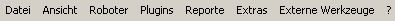
\includegraphics[width=1\textwidth]{images/menu}
    \caption{Das Men�}
    \label{img:workspace:menu}
\end{figure}

Wie zu sehen ist, gibt es acht verschiedene Eintr�ge, welche nun im Einzelnen
erl�utert werden.

\subsection{Datei}
\index{Arbeitsbereich!Men�!Datei}
\index{Kommunikationsspezifikationsdatei}
\index{Roboterdatei}

Das Men� \enquote{Datei} enth�lt acht Eintr�ge. Allerdings sind von diesen in
der Version 2.4.0 nur vier verf�gbar, da momentan noch keine Editoren f�r
Roboter- und Kommunikationsspezifikationsdateien existieren
\footnote{Es ist geplant, dass diese Editoren ab der Version 3.0.0 verf�gbar
seien werden.}. Daher fallen die Eintr�ge \texttt{Neuer Roboter},
\texttt{Roboter bearbeiten}, \texttt{Neue Kommunikationsspezifikation} und
\texttt{Kommunikationsspezifikation bearbeiten} weg. Die restlichen vier
Eintr�ge werden im folgenden beschrieben.

\subsubsection{Neues Profil}
\index{Profile!Profileditor}
Wird dieser Eintrag ausgew�hlt, �ffnet sich der Profileditor im Modus zum
Erstellen eines neuen Profils.

\subsubsection{Profil bearbeiten}
\index{Profile!Profileditor}
Wird dieser Eintrag ausgew�hlt, �ffnet sich der Profileditor im Modus zum
Bearbeiten eines bereits kompletten, oder eines nicht kompletten Profils.

\subsubsection{Einstellungen}
\index{Einstellungen}
Die Auswahl dieses Eintrages �ffnet den Einstellungsdialog. Mehr �ber die
vorhandenen Einstellungsm�glichkeiten kann im Kapitel \enquote{Einstellungen}
ab Seite \pageref{ref:settings} nachgelesen werden.

\subsubsection{Beenden}
Wird dieser Eintrag gew�hlt schlie�t sich die Anwendung.

\subsection{Ansicht}
\index{Arbeitsbereich!Men�!Ansicht}

Das Men� \enquote{Ansicht} enth�lt sieben Optionen die aktiviert oder
deaktiviert werden k�nnen. Jeder dieser Optionen bewirkt ein sichtbare �nderung
im Arbeitsbereich.

\subsubsection{C.O.P. sichtbar}
\index{Kontroll�bersicht}
Diese Option ist nur verf�gbar, wenn mindestens ein Profil mit mehr als einem
Roboter geladen wurde. Wird die Option aktiviert ist die Kontroll�bersicht als
weiterer Reiter auf der Profil-Reiter Ebene verf�gbar. Wird die Option
deaktiviert wird auch die Kontroll�bersicht geschlossen.

\subsubsection{Werkzeuge sichtbar}
Wird diese Option aktiviert ist die Anwendungswerkzeugleiste sichtbar, wird sie
deaktiviert wird diese unsichtbar und stellt dem Arbeitsbereich etwas mehr
Platz zur Verf�gung.

\subsubsection{Werkzeuge arretiert}
Wird diese Option aktiviert wird die Anwendungswerkzeugleiste arretiert, wird
sie deaktiviert ist es m�glich die Werkzeuge in der Werkzeugleiste zu
verschieben.

\subsubsection{Statusleiste sichtbar}
Wird diese Option aktiviert ist die Statusleiste sichtbar,wird sie
deaktiviert wird diese unsichtbar und stellt dem Arbeitsbereich etwas  mehr
Platz zur Verf�gung.

\subsubsection{Systemprotokolle sichtbar}
\index{Systemprotokoll}
Wird diese Option aktiviert sind in allen vorhandenen Roboter-Reitern die
Systemprotokolle\footnote{Ab Version 3.0.0 wird diese Option profilabh�ngig. So
werden nicht alle Systemprotokolle aus allen Reitern entfernt, sondern nur f�r
ein bestimmtes Profil.} sichtbar, wird sie deaktiviert werden die Protokolle
nicht angezeigt.

\subsubsection{Live-Diagramme sichtbar}
\index{Live-Diagramme}
Wird diese Option aktiviert sind in allen vorhandenen Roboter-Reitern die
Live-Diagramme\footnote{Ab Version 3.0.0 wird diese Option profilabh�ngig. So
werden nicht alle Live-Diagramme aus allen Reitern entfernt, sondern nur f�r
ein bestimmtes Profil.} sichtbar, wird sie deaktiviert werden die
Live-Diagramme nicht angezeigt.

\subsubsection{Rekorder sichtbar}
\index{Rekorder}
Wird diese Option aktiviert sind in allen vorhandenen Roboter-Reitern die
Rekorder\footnote{Ab Version 3.0.0 wird diese Option profilabh�ngig. So
werden nicht alle Rekorder aus allen Reitern entfernt, sondern nur f�r
ein bestimmtes Profil.} sichtbar, wird sie deaktiviert werden die Rekorder nicht
angezeigt.

\subsubsection{Roboter�bersicht sichtbar}
\index{Roboter�bersicht}
Wird diese Option aktiviert sind in allen vorhandenen Roboter-Reitern die
Roboter�bersicht\footnote{Ab Version 3.0.0 wird diese Option profilabh�ngig. So
werden nicht alle Roboter�bersichten aus allen Reitern entfernt, sondern nur f�r
ein bestimmtes Profil.} sichtbar, wird sie deaktiviert werden die
Roboter�bersichten nicht angezeigt.

\subsection{Roboter}
\index{Arbeitsbereich!Men�!Roboter}
Das Men� \enquote{Roboter} ist ein dynamisch beim Start der Anwendung erstelltes
Men�. Es enth�lt f�r jedes erfolgreich geladene Profil einen eigenen Eintrag.
�ffnet man eines dieser Men�s wird f�r jeden Roboter des Profils eine Option
angezeigt\footnote{Ab Version 3.0.0 wird es die M�glichkeit geben den Zustand
des Profils bei Beenden der Anwendung im Profil zu speichern.}. Ist diese Option
aktiviert wird der entsprechende Roboter-Reiter angezeigt, wird sie deaktiviert wird
der Roboter-Reiter geschlossen.

\subsection{Plugins}
\index{Arbeitsbereich!Men�!Plugins}
\index{Plugins}
\index{Einstellungen}
Das Men� \enquote{Plugins} ist ein dynamisches, kontextsensitives Men�. Es ist
abh�ngig von dem aktuell aktivem Roboter. Es enth�lt Eintr�ge f�r die Plugins
des Roboters, welche entweder keine graphische Benutzeroberfl�che haben und nur
eine Funktionalit�t ausf�hren, oder solche die zwar eine graphische
Benutzeroberfl�che besitzen, aber nicht eingebettet in den Arbeitsbereich
dargestellt werden sollen, sondern in Dialogform in einem eigenen Fenster.
Des Weiteren enth�lt dieses einen Eintrag der die Einstellungen �ffnet.

\subsection{Reporte}
\index{Arbeitsbereich!Men�!Reporte}
\index{Reporte}
\index{Reporte!PDF}
\index{Plugins}
Das Men� \enquote{Reporte} ist ein dynamisches, kontextsensitives Men�. Es ist
abh�ngig von dem aktuell aktivem Roboter. Es enth�lt Eintr�ge f�r die
Report-Plugins des Roboters, sowie einen Eintrag zum �ffnen des Suchdialogs f�r
Reporte. Wird ein Report erzeugt, wird dieser nach der Erstellung sofort im
\seegls{PDF}-Betrachter des Betriebssystems ge�ffnet.

\subsection{Extras}
\index{Arbeitsbereich!Men�!Extras}
Das Men� \enquote{Extras} enth�lt Eintr�ge f�r diverse zus�tzliche Funktionen
die in \xirp~verf�gbar sind.

\subsubsection{Mail}
\index{Mail}
Wird dieser Eintrag gew�hlt �ffnet sich die Mailverwaltung der Anwendung.

\subsubsection{Kontakte}
\index{Kontakte}
Wird dieser Eintrag gew�hlt �ffnet sich die Kontaktverwaltung der Anwendung.

\subsubsection{Diagramme}
\index{Diagramme}
Wird dieser Eintrag gew�hlt �ffnet sich der Dialog zum Konfigurieren des
Diagrammgenerators.

\subsubsection{Testerbot ausf�hren}
\index{Testerbot}
Wird dieser Eintrag gew�hlt �ffnet sich der Kontrolldialog des \seegls{Testerbot}
\seegls{Server}s.

\subsection{Externe Werkzeuge}
\index{Arbeitsbereich!Men�!Externe Werkzeuge}
\index{Externe Werkzeuge}
Das Men� \enquote{Externe Werkzeuge} ist ein dynamisches, kontextsensitives
Men�. Es ist abh�ngig vom aktuell aktivem Profil. Es enth�lt f�r jedes im Profil
spezifiziertes externes Werkzeug einen Eintrag mit dem angegebenen Namen des
Werkzeugs. Wird ein Eintrag ausgew�hlt werden die in dem externen Werkzeug
angegebenen Programme in der gewollten Reihenfolge und in dem angegebenen
zeitlichen Abstand gestartet.

\subsection{?}
\index{Arbeitsbereich!Men�!?}
Das Men� \enquote{?} enth�lt Eintr�ge zum Anzeigen von Programminformationen und
der Hilfe zur Anwendung und den Plugins.

\subsubsection{�ber \xirp~2}
Wird dieser Eintrag gew�hlt �ffnet sich ein Informationsdialog, der die aktuelle
Versionnummer anzeigt.

\subsubsection{�ber Plugins}
\index{Plugins}
Wird dieser Eintrag gew�hlt �ffnet sich ein Dialog, der Informationen �ber die
geladenen Plugins anzeigt.

\subsubsection{Hilfe}
\index{Hilfe}
Wird dieser Eintrag gew�hlt �ffnet sich die Hilfe zu \xirp~und den geladenen Plugins.

\section{Anwendungswerkzeugleiste}
\index{Arbeitsbereich!Anwendungswerkzeugleiste}
Die Werkzeugleiste der Anwendung ist in Abbildung \ref{img:workspace:apptools} auf Seite
\pageref{img:workspace:apptools} zu sehen.

\begin{figure}[ht]
    \centering
    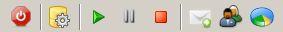
\includegraphics[width=.75\textwidth]{images/apptools}
    \caption{Die Anwendungswerkzeugleiste}
    \label{img:workspace:apptools}
\end{figure}

Wie zu sehen ist, gibt es acht verschiedene Werkzeugelemente. In Tabelle
\ref{tab:apptools} auf Seite \pageref{tab:apptools} werden diese Elemente
genauer erkl�rt.

\begin{table}[htpb]
    \centering
    \begin{tabular}{c|l}
    Werkzeugelement & Beschreibung\\
    \hline
    
\includegraphics{images/quit} & Auswahl des Elements schlie�t die
    Anwendung.\\
    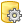
\includegraphics{images/preferences} & Auswahl des Elements
    �ffnet den Einstellungsdialog.\\
    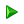
\includegraphics{images/start} & Auswahl des Elements startet alle Stoppuhren.\\
    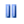
\includegraphics{images/pause} & Auswahl des Elements pausiert alle Stoppuhren.\\
    
\includegraphics{images/stop} & Auswahl des Elements stoppt alle Stoppuhren.\\
    
\includegraphics{images/send_mail} & Auswahl �ffnet die Mailverwaltung.\\
    
\includegraphics{images/contacts} & Auswahl �ffnet die Kontaktverwaltung.\\
    
\includegraphics{images/chart} & Auswahl �ffnet den Dialog zum Konfigurieren des\\
    & Diagrammgenerators.\\
    \end{tabular}
    \caption{Die Elemente der Anwendungswerkzeugleiste}
    \label{tab:apptools}
    \index{Einstellungen}
    \index{Mail}
    \index{Kontakte}
    \index{Stoppuhr}
\end{table}

\section{Roboterwerkzeugleiste}
\index{Arbeitsbereich!Roboterwerkzeugleiste}
Die Werkzeugleiste der Roboter ist in Abbildung \ref{img:workspace:robtools} auf Seite
\pageref{img:workspace:robtools} zu sehen.

\begin{figure}[ht]
    \centering
    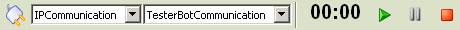
\includegraphics[width=1\textwidth]{images/robottools}
    \caption{Die Roboterwerkzeugleiste}
    \label{img:workspace:robtools}
\end{figure}

\index{Plugins}
Wie zu sehen ist, gibt es sieben verschiedene Werkzeugelemente. In Tabelle
\ref{tab:robottools} auf Seite \pageref{tab:robottools} werden diese Elemente
genauer erkl�rt. Diese Elemente sind f�r jeden Roboter verf�gbar. Plugins k�nnen
allerdings Werkzeugleisten definieren die dann zus�tzlich dort angezeigt werden.

\begin{table}[htpb]
    \centering
    \begin{tabular}{c|l}
    Werkzeugelement & Beschreibung\\
    \hline
    
\includegraphics{images/not_connected} & Auswahl des Elements stellt eine
    Verbindung\\
    & zu dem Roboter mit den eingestellten Optionen her.\\
    & Ist eine Verbindung hergestellt kann durch eine weitere\\
    & Auswahl des Elements die Verbindung getrennt werden.\\
    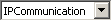
\includegraphics{images/medium} & Auswahl des Kommunikationsmediums.\\
    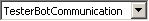
\includegraphics{images/protocol} & Auswahl des Kommunikationsprotokolls.\\
    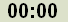
\includegraphics{images/watch} & Die Stoppuhranzeige.\\
    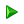
\includegraphics{images/start} & Auswahl des Elements startet die Stoppuhr\\
    & des Roboters.\\
    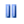
\includegraphics{images/pause} & Auswahl des Elements pausiert die Stoppuhr\\
    & des Roboters.\\
    
\includegraphics{images/stop} & Auswahl des Elements stoppt die Stoppuhr\\
    & des Roboters.\\
    \end{tabular}
    \caption{Die Elemente der Roboterwerkzeugleiste}
    \label{tab:robottools}
    \index{Stoppuhr}
\end{table}

\newpage

\section{Statusleiste}
\index{Arbeitsbereich!Statusleiste}
\index{Kontroll�bersicht}
Die Statusleiste der Anwendung ist kontextsensitiv. Sie ist abh�ngig vom aktuell
aktivem Roboter und dem Verbindungsstatus des Roboters, oder dem Kontroll�bersicht.
In den Abbildungen \ref{img:workspace:statusnc} (Seite \pageref{img:workspace:statusnc}),
\ref{img:workspace:statusc} (Seite \pageref{img:workspace:statusc})
und \ref{img:workspace:statuscop} (Seite \pageref{img:workspace:statuscop}) sind
die drei verschiedenen Zust�nde der Statusleiste zu sehen.
\par
Die Statusleiste zeigt die folgenden Informationen �ber den aktuellen Roboter
von links nach rechts an:

\begin{itemize}
  \item Robotername
  \item Verbindungsstatus
  \item Information �ber den Kontrollstatus
  \item Anzeige �ber die gesendete und empfangene Datenmenge
  \item Anzeige des Status der Energiequelle
\end{itemize}

Wenn der Kontroll�bersicht ge�ffnet ist zeigt die Statusleiste die folgenden
Informationen von links nach rechts an:

\begin{itemize}
  \item Information, dass mehrere Roboter gesteuert werden
  \item Weiterer Informationstext
  \item Anzeige �ber die gesendete und empfangene Datenmenge
\end{itemize}

\begin{figure}[ht]
    \centering
    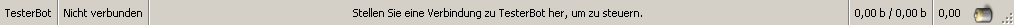
\includegraphics[width=1\textwidth]{images/statusnc}
    \caption{Die Statusleiste im \enquote{nicht verbundenen} Zustand}
    \label{img:workspace:statusnc}
\end{figure}

\begin{figure}[ht]
    \centering
    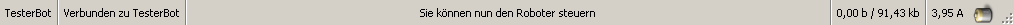
\includegraphics[width=1\textwidth]{images/statusc}
    \caption{Die Statusleiste im \enquote{verbundenen} Zustand}
    \label{img:workspace:statusc}
\end{figure}

\begin{figure}[ht]
    \centering
    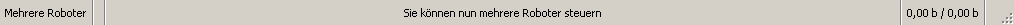
\includegraphics[width=1\textwidth]{images/statuscop}
    \caption{Die Statusleiste im \enquote{Kontroll�bersicht} Zustand}
    \label{img:workspace:statuscop}
\end{figure}

\section{Hauptarbeitsbereich}
\index{Arbeitsbereich!Hauptarbeitsbereich}
Der Hauptarbeitsbereich besteht aus mehreren Reitern. Jeder Reiter entspricht
einem geladenen Profil. Diese Reiter tragen den Namen des geladenen Profils.
In Abbildung \ref{img:tab:profile} auf Seite \pageref{img:tab:profile} ist dies
rot markiert.
\par
Jeder dieser Reiter enth�lt weitere Reiter. F�r jeden im Profil enthaltenen
Roboter einen weiteren Reiter. In Abbildung \ref{img:tab:robot} auf Seite
\pageref{img:tab:robot} ist dies rot markiert.

\begin{figure}[ht]
    \centering
    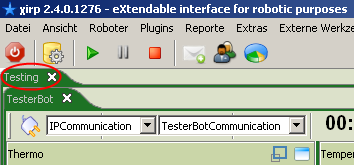
\includegraphics[width=.75\textwidth]{images/profiletab}
    \caption{Die Profil-Reiter}
    \label{img:tab:profile}
\end{figure}

\begin{figure}[ht]
    \centering
    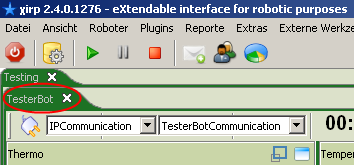
\includegraphics[width=.75\textwidth]{images/robottab}
    \caption{Die Roboter-Reiter}
    \label{img:tab:robot}
\end{figure}

\index{Kontroll�bersicht}
Der Kontroll�bersicht wird auf der Ebene der Profil-Reiter in einem eigenen
Reiter dargestellt.


\subsection{Drag-and-Drop der enthaltenen Elemente}
\index{Plugins}
Der Arbeitsbereich eines Roboters setzt sich aus den Standard Elementen und den
Plugin Elementen zusammen. Die Elemente k�nnen frei in diesem Bereich angeordnet
werden. Mittels \seegls{Drag-and-Drop} kann die Anordnung der Elemente ver�ndert werden.
Um z.B. Element \enquote{A} links neben Element \enquote{B} zu verschieben muss
die Maus �ber der Titelzeile des Element gehalten und dann auf die
Trennlinie links neben Element \enquote{B} verschoben und dann
\enquote{losgelassen} werden. Pfeile zeigen an, ob ein Element an der
gew�nschten Stelle eingef�gt werden kann. Es ist ebenfalls m�glich Elemente
�bereinander zu \enquote{stapeln} in dem das Element einfach �ber einem andern
\enquote{losgelassen} wird.

\subsection{Anzeigem�glichkeiten der Elemente}
Einige der Standard Elemente und Plugins k�nnen bei Bedarf in einem eigenen
Fenster angezeigt werden. Um dieses zu erreichen muss auf das \enquote{in
eigenem Fester anzeigen} \seegls{Icon} geklickt werden. Das \seegls{Icon} ist in Abbildung
\ref{img:windowed} auf Seite \pageref{img:windowed} rot markiert. Die Abbildung
zeigt ebenfalls, wie ein Plugin in einem eigenen Fenster angezeigt wird. Das
Plugin wird, wenn das Fenster geschlossen wird, wieder an seine urspr�ngliche
Stelle im Arbeitsbereich eingef�gt.

\begin{figure}[ht]
    \centering
    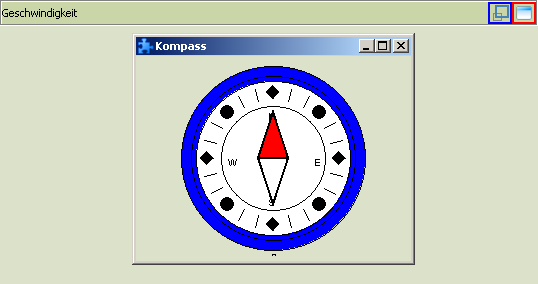
\includegraphics[width=.75\textwidth]{images/windowed}
    \caption{Ein Plugin in eigenen Fenster}
    \label{img:windowed}
\end{figure}

Es ist ebenfalls m�glich ein Element zu \enquote{maximieren}. Wenn das in Abbildung
\ref{img:windowed} auf Seite \pageref{img:windowed} blau markierte \seegls{Icon}
angeklickt wird, nimmt das Element den kompletten Platz des
Roboterarbeitsbereich ein. Dies ist in Abbildung \ref{img:maximized} auf Seite
\pageref{img:maximized} zu sehen. In dieser Abbildung ist rechts oben das \seegls{Icon}
zum Wiederherstellen der Originalgr��e rot markiert.

\begin{figure}[ht]
    \centering
    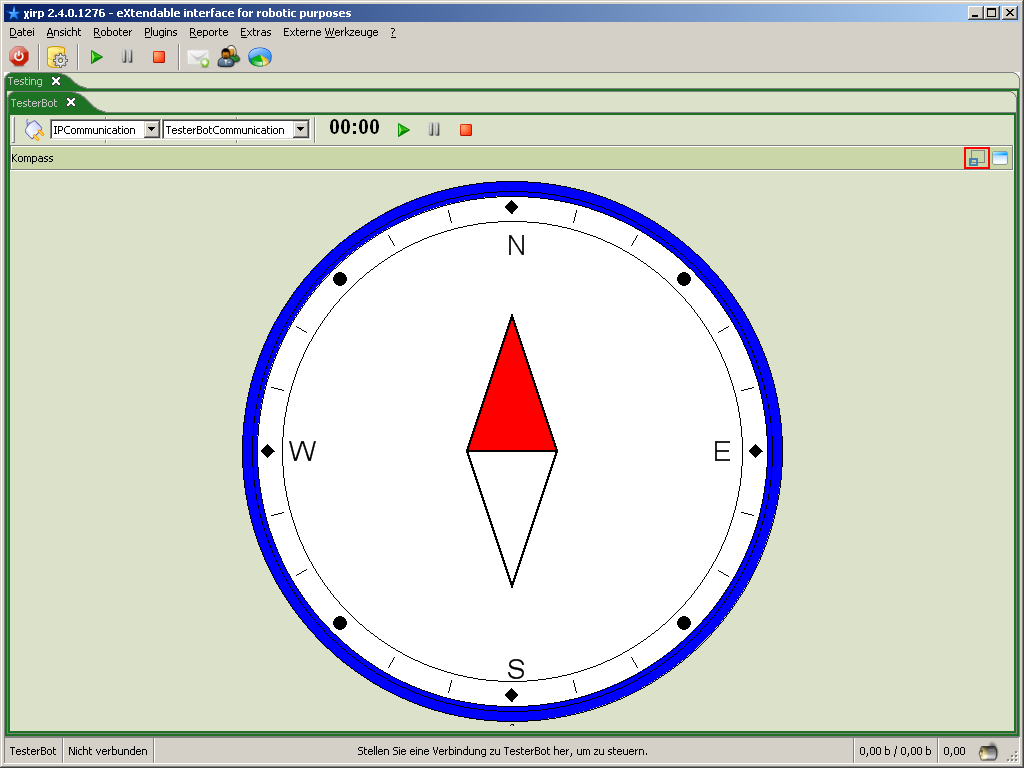
\includegraphics[width=1\textwidth]{images/fullscreen}
    \caption{Ein maximiertes Plugin}
    \label{img:maximized}
\end{figure}

\index{Arbeitsbereich|)}

\chapter{Einstellungen}
\index{Einstellungen|(}
\index{Plugins}
\label{ref:settings}

In \xirp~existiert eine einzelne Stelle, wenn es um Einstellungen f�r die
Anwendung und der darin geladenen Plugins geht, der Dialog 
\enquote{Einstellungen}. Die Einstellungen der Anwendung sind in die folgenden
neun Kategorien eingeteilt.

\begin{itemize}
  \item Allgemeine Einstellungen
  \item Erscheinungsbild
  \item Spracheinstellungen
  \item Tastenk�rzel
  \item Externe Werkzeuge
  \item Datenbankeinstellungen
  \item Maileinstellungen
  \item Speech-Einstellungen
  \item Diagrammeinstellungen
\end{itemize}

Jedes Plugin kann Einstellungen definieren. Wenn dies der Fall ist, erh�lt das
Plugin in einer Einstellungsgruppe des Roboters eine eigene Kategorie unter der
sich die Einstellungen des Plugins befinden. Das folgende Kapitel erl�utert alle
existierenden Einstellungsm�glichkeiten und gibt einen Einblick in den Dialog
mit dem diese Einstellungen get�tigt werden k�nnen.

\newpage

\section{Einstellungsdialog}

Der Dialog zum Vornehmen der systemweiten und pluginspezifischen Einstellungen
ist in einen Kategorie- und einen Inhaltsbereich aufgeteilt. Der
Kategoriebereich ist in Abbildung \ref{img:settings:dialog} auf Seite
\pageref{img:settings:dialog} rot und der Inhaltsbereich blau markiert.

\begin{figure}[ht]
    \centering
    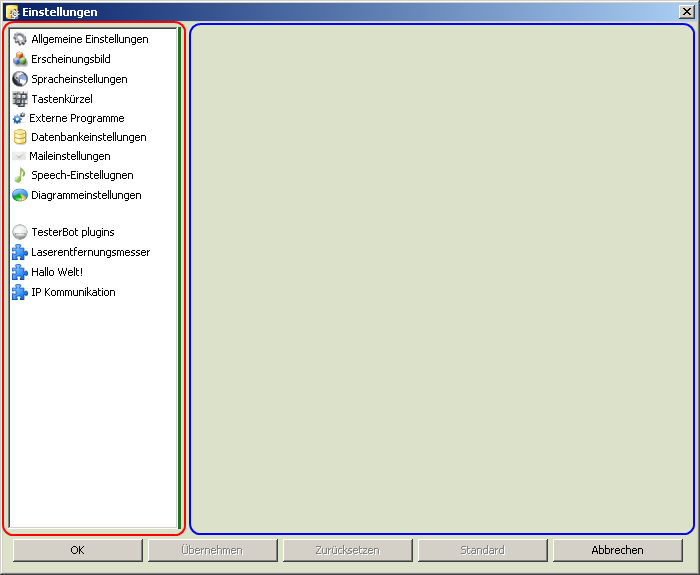
\includegraphics[width=1\textwidth]{images/settingsdialog}
    \caption{Der Settingsdialog mit markierten Kategorie- und Inhaltsbereichen}
    \label{img:settings:dialog}
\end{figure}

Um die Einstellungen einer Kategorie oder eines Plugins vorzunehmen, muss durch
einen Klick auf das entsprechende Listenelement auf der linken Seite der Inhalt
aufgerufen werden. In der Abbildung \ref{img:settings:content}
auf Seite \pageref{img:settings:content} ist der Inhalt f�r
\enquote{Allgemeinen Einstellungen} zu sehen.

\begin{figure}[hp]
    \centering
    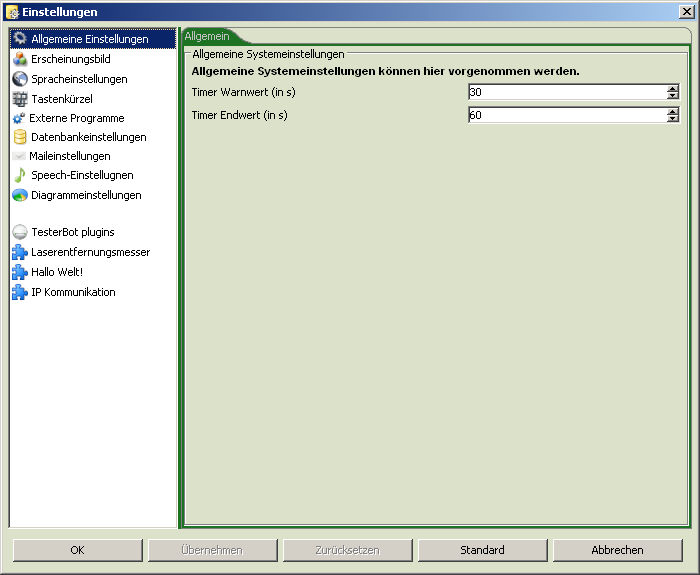
\includegraphics[width=1\textwidth]{images/settingscontent}
    \caption{Der Settingsdialog mit ge�ffnetem \enquote{Allgemeine Einstellungen}
    Inhalt}
    \label{img:settings:content}
\end{figure}

\newpage

Wie in den Abbildungen zu sehen gibt es diverse Kn�pfe die man anklicken k�nnte.

\begin{itemize}
  \item \texttt{OK}, speichert die neuen Einstellungen und schie�t den Dialog
  \item \texttt{�bernehmen}, speichert die neuen Einstellungen
  \item \texttt{Zur�cksetzen}, setzt auf den zuletzt gespeicherten Wert zur�ck
  \item \texttt{Standard}, setzt den Wert auf seinen Standard Wert
  \item \texttt{Abbrechen}, verwirft alle neuen Einstellungen und schlie�t den Dialog
\end{itemize}

\texttt{Zur�cksetzen} und \texttt{Standard} sind nur verf�gbar, wenn die Funktion
von den Einstellungen unterst�tzt wird.

In den folgenden Abschnitten werden die einzelnen Einstellungsm�glichkeiten der
Anwendung erl�utert.

\section{Allgemeine Einstellungen}
In den allgemeinen Einstellungen gibt es zwei Werte die einstellbar sind.

\begin{itemize}
  \item Timer Warnwert
  \item Timer Endwert
\end{itemize}

Die Werte f�r diese Einstellungen werden in Sekunden angegeben. Sie werden bei
der Farbberechnung der Stoppuhr Anzeige benutzt. Nach den im Warnwert
angegebenen Sekunden wechselt die Anzeige ihre Farbe nach orange. Wird der
Endwert erreicht, wechselt die Anzeige ihre Farbe nach rot.

\section{Erscheinungsbild}
In den Einstellungen f�r das Erscheinungsbild der Anwendung gibt es sieben
Farboptionen.

\begin{itemize}
  \item Reiterfarbe
  \item Reiterschriftfarbe
  \item Textfarbe eines inaktiven Reiters
  \item Farbe f�r diverse Elemente die den Fokus haben
  \item Trennlinienfarbe
  \item Hintergrundfarbe
  \item Farbe der Elementtitel
\end{itemize}

Eine Demonstration der Farbenwerte kann in Abbildung \ref{img:settings:badcolor}
auf Seite \pageref{img:settings:badcolor} betrachtet werden.

\begin{figure}[ht]
    \centering
    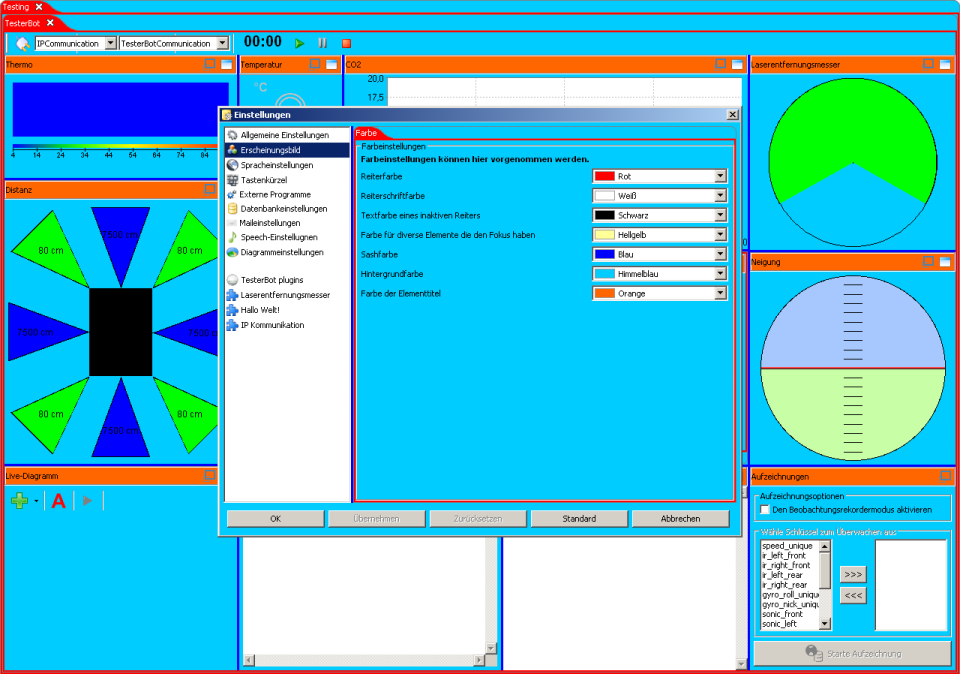
\includegraphics[width=1\textwidth]{images/badcolors}
    \caption{\xirp~mit abweichender Kolorierung zum Verdeutlichung der Farboptionen}
    \label{img:settings:badcolor}
\end{figure}

\section{Spracheinstellungen}
\index{Internationalisierung}
In den Spracheinstellungen gibt es nur eine Option: Die zu verwendende Sprache
der Anwendung. \xirp~unterst�tzt momentan die folgenden Sprachen. Weitere
Sprachpakete sollen in Zukunft folgen.

\begin{itemize}
  \item Deutsch
  \item Englisch
\end{itemize}

Die eingestellte Sprache gilt sowohl f�r die Anwendung als auch f�r die
geladenen Plugins. Sollte ein Plugin f�r die eingestellte Sprache keine
Sprachdatei zur Verf�gung stellen wird die Standard Sprache des Plugins
benutzt.

\section{Tastenk�rzel}
Die Kategorie \enquote{Tastenk�rzel} enth�lt zwei Typen von Tastenk�rzeln.

\begin{itemize}
  \item Anwendungsk�rzel, z.B. Strg+Q
  \item Kommandok�rzel
\end{itemize}

\subsection{Anwendungsk�rzel}
\index{Hotkey}
Die Anwendungsk�rzel werden benutzt um oft benutzte Funktionen mittels einer
Tastenkombination verf�gbar zu machen. In \xirp~gibt es diverse Tastenk�rzel. In
den Einstellungen gibt es eine Aufteilung nach den Tasten vor dem eigentlichen
\seegls{Hotkey}.

\begin{itemize}
  \item Strg+
  \item Strg+Umschalt+
  \item Strg+Alt+
\end{itemize}

F�r jede dieser 3 M�glichkeiten existiert ein eigener Reiter auf der Inhaltsseite
der Einstellungen. Die einzelnen verf�gbaren Funktionen werden im folgenden
erl�utert.

\newpage

\subsubsection{Strg+ - Tastenk�rzel}
\index{Hotkey}
Es existieren sieben Funktionen deren Tastenk�rzel frei bestimmt werden kann.
Der \enquote{\seegls{Hotkey}} wird nach der Steuerung-Taste (Strg) erwartet.

\begin{itemize}
  \item Programm beenden
  \item Einstellungen �ffnen
  \item Hilfe anzeigen
  \item Mailverwaltung �ffnen
  \item Konfigurationsdialog f�r den Diagrammgenerator �ffnen
  \item Reportsuche �ffnen
  \item Kontaktverwaltung �ffnen
\end{itemize}

\subsubsection{Strg+Umschalt+ - Tastenk�rzel}
\index{Hotkey}
Es existiert eine Funktion deren Tastenk�rzel frei bestimmt werden kann.
Der \enquote{\seegls{Hotkey}} wird nach der Steuerung- plus der Umschalt-Taste
(Strg+Umschalt) erwartet.

\begin{itemize}
  \item Programminformationen anzeigen
\end{itemize}

\subsubsection{Strg+Alt+ - Tastenk�rzel}
Es existiert eine Funktion deren Tastenk�rzel frei bestimmt werden kann.
Der \enquote{\seegls{Hotkey}} wird nach der Steuerung- plus der Alt-Taste
(Strg+Alt) erwartet.

\begin{itemize}
  \item Plugininformationen anzeigen
\end{itemize}

\subsection{Kommando Tastenk�rzel}
\index{Kommandos}
\index{Kommandos!kommandierbar}
\index{Gamepad}
Plugins k�nnen kommandierbar sein, das bedeutet, dass ein Plugin/eine Klasse
gewissen Funktionen f�r Kommandos freigeben kann. Zum Beispiel k�nnte eine
\enquote{Notaus} Funktion freigegeben werden. Um diese Funktion nutzen zu
k�nnen muss f�r die Funktion entweder eine Taste der Tastatur, eine Taste eines
\seegls{Gamepad}s, oder beides hinterlegt werden. Dies kann in dem Inhaltsreiter
\enquote{Kommando Tastenk�rzel} getan werden. Die dort vorhandene Tabelle
enth�lt alle verf�gbaren Kommando-Funktionen (Siehe Abbildung
\ref{img:settings:commads} auf Seite \pageref{img:settings:commads}).

\begin{figure}[hbp]
    \centering
    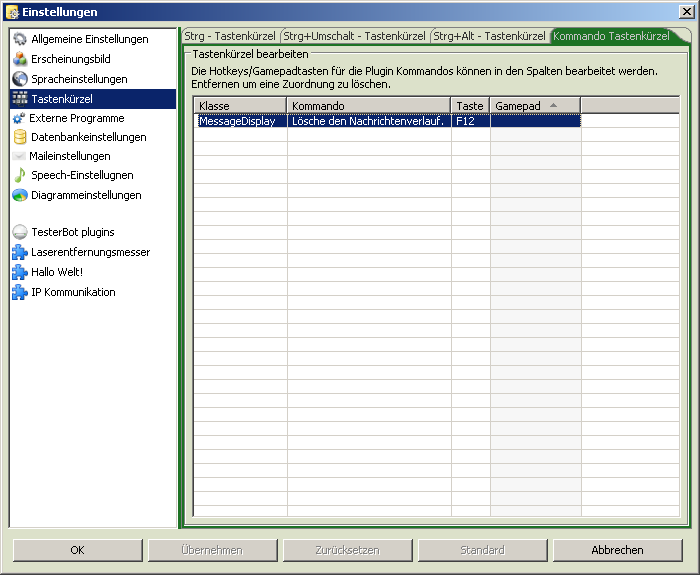
\includegraphics[width=1\textwidth]{images/commands}
    \caption{Kommando Tastenk�rzel Konfiguration}
    \label{img:settings:commads}
\end{figure}

Wie zu sehen ist, wurde der Funktion \enquote{L�sche den Nachrichtenverlauf.}
der Klasse \enquote{MessageDisplay} die Tastaturtaste \enquote{F12} zugewiesen.
Eine Gamepadtaste wurde noch nicht zugewiesen. Um nun die Taste zu �ndern oder
hinzuzuf�gen muss nur auf die entsprechende Tabellenzelle geklickt werden. Hier
�ffnet sich nun ein Eingabefeld. Dann muss nur noch die gew�nschte
Tastatur-/Gamepadtaste gedr�ckt werden.

\section{Externe Werkzeuge}
\index{Externe Werkzeuge}
In den Einstellungen f�r die externen Programme der \seegls{Profile} gibt es pro
geladenem Profil einen Inhaltsreiter. Jeder dieser Reiter enth�lt die
Konfigurationsoberfl�che die in Abbildung \ref{img:settings:ext} auf Seite
\pageref{img:settings:ext} zu sehen ist.

\begin{figure}[hp]
    \centering
    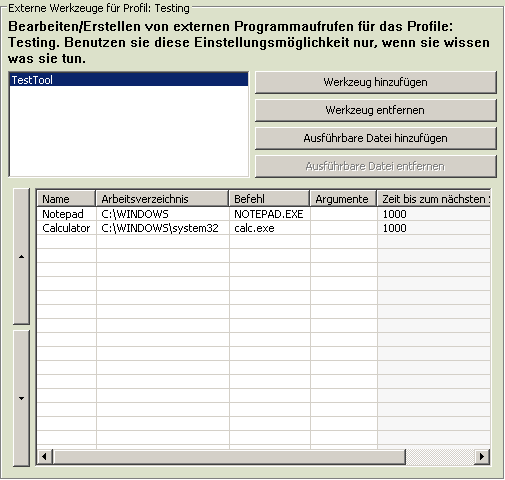
\includegraphics[width=.75\textwidth]{images/ext}
    \caption{Oberfl�che zum konfigurieren der externen Programme}
    \label{img:settings:ext}
\end{figure}

Um ein neues externes Werkzeug anzulegen muss einfach auf den Knopf
\enquote{Werkzeug hinzuf�gen} geklickt werden. Dann muss in dem folgenden
Eingabedialog der Name des Werkzeugs angegeben werden. Ist dies erfolgreich
wird in der List das neue Werkzeug angezeigt. Der n�chste Schritt ist nun diesem
Werkzeug mindestens ein ausf�hrbares Programm zuzuordnen. Dazu muss zuerst das
Werkzeug in der Liste markiert werden und dann auf den Knopf
\enquote{Ausf�hrbare Datei hinzuf�gen} geklickt werden.
\par
Der folgende Eingabedialog erwartet zwei Pflichtangaben: Den Namen des Programms
und die Wartezeit nach Start der Anwendung. Der Name des Programms ist frei
w�hlbar. In dem Beispiel in Abbildung \ref{img:settings:ext:example} auf Seite
\pageref{img:settings:ext:example} ist als Name \enquote{Firefox} gew�hlt. Die
Wartezeit nach dem Start wird in Millisekunden angegeben. Dieser Wert kann
genutzt werden, um einem Programm eine gewissen zeitlichen Spielraum zu
verschaffen, bis ein weiteres gestartet wird. Dies ist n�tzlich falls
nachfolgende Programme von vorherigen abh�ngig sind.

\begin{figure}[hp]
    \centering
    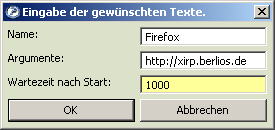
\includegraphics[width=0.5\textwidth]{images/ext_example}
    \caption{Beispieleingabe f�r ein ausf�hrbares Programm}
    \label{img:settings:ext:example}
\end{figure}

Die \enquote{Argumente} Eingabe ist optional. Hier k�nnen Argumente angegeben
werden die ein Programm beim Start ben�tigt. Wird dieser Eingabedialog best�tigt
erscheint ein Dateiauswahldialog. Erst jetzt wird die eigentliche ausf�hrbare
Datei ausgew�hlt.
\par
Wurden zu einem Werkzeug mehrere Programme hinzugef�gt kann die Reihenfolge in
der sie gestartet werden sollen mittels der Pfeiltasten auf der linken Seiten
ver�ndert werden.

\section{Datenbankeinstellungen}
\index{Datenbank}
In den Einstellungen f�r die Datenbank gibt es f�nf Optionen die eingestellt
werden k�nnen.

\begin{itemize}
  \item IP-Adresse
  \item Port
  \item Benutzer
  \item Passwort
  \item Datenbanktreiber
\end{itemize}

\newpage

Die ersten vier Optionen beziehen sich auf Datenbanken die �ber \seegls{TCP/IP}
kommunizieren. Diese sollten angegeben werden, wenn ein Datenbanktreiber gew�hlt
wird der diese Einstellungen ben�tigt. Momentan werden die folgenden Datenbanken
unterst�tzt.

\begin{itemize}
  \item HSQLDB
  \item MySQL
\end{itemize}

\index{Rekorder}
\index{Reporte}
Die \enquote{HSQSLDB} wird bei der Installation von \xirp~mitgeliefert, so dass
kein spezieller Datenbankserver vorhanden sein muss, um Aufzeichnungen mit dem
Rekorder vorzunehmen und Reporte abzuspeichern.

\section{Maileinstellungen}
\index{Mail}
In den Einstellungen f�r das Mailsystem gibt es sechs Optionen die eingestellt
werden k�nnen.

\begin{itemize}
  \item SMTP-Host
  \item Port
  \item Authentifizierung n�tig
  \item Benutzername
  \item Passwort
  \item No-Reply Adresse
\end{itemize}

Hier k�nnen die f�r die Kommunikation mit dem SMTP-\seegls{Server} n�tigen Einstellungen
gemacht werden. Die \enquote{No-Reply} Adresse muss gesetzt werden, da sonst das
Versenden von E-Mails nicht funktionieren wird.

\section{Speech-Einstellungen}
\index{Text-To-Speech}
\index{Sprachausgabe}
In den Einstellungen f�r das Speech-System\footnote{Bisher wird nur
Sprachausgabe unterst�tzt. Spracherkennung soll in einer zuk�nftigen Version
hinzukommen} gibt es zwei Optionen die eingestellt werden k�nnen.

\begin{itemize}
  \item Stimme der Sprachausgabe
  \item Sprachausgabe aktivieren
\end{itemize}

Die erste Option bestimmt die Stimme die f�r die Sprachausgabe benutzt werden
soll. Es gibt zwei Standard Sprachen:

\begin{itemize}
  \item kevin
  \item kevin16
\end{itemize}

Das Sprachausgabesystem unterst�tzt \enquote{MBROLA} Stimmen. Wenn diese
installiert werden, werden die neu hinzugekommenen Stimmen ebenfalls hier zur
Auswahl gestellt. in Kapitel \ref{ref:speech} ab Seite \pageref{ref:speech} kann
nachgelesen werden, wie diese zus�tzlichen Stimmen installiert werden k�nnen und
woher man diese beziehen kann.

\section{Diagrammeinstellungen}
\label{ref:settings:livechart}
\index{Live-Diagramme}
\index{Live-Diagramme!PDF}
\index{Live-Diagramme!PNG}
\index{Live-Diagramme!JPG}
\index{Live-Diagramme!CSV}
In den Einstellungen f�r die Live-Diagramme gibt es vier Optionen die eingestellt
werden k�nnen. Alle beziehen sich darauf, ob nach dem Stoppen eines
Plottingvorgangs das erzeugte Diagramm in verschiedenen Formaten automatisch
exportiert werden sollen.

\begin{itemize}
  \item PDF beim Stoppen eines Live-Diagramms automatisch exportieren
  \item PNG beim Stoppen eines Live-Diagramms automatisch exportieren
  \item JPG beim Stoppen eines Live-Diagramms automatisch exportieren
  \item CSV beim Stoppen eines Live-Diagramms automatisch exportieren
\end{itemize}

\index{Einstellungen|)}

\chapter{Mail- und Kontaktverwaltung}
\index{Mail|(}
\index{Kontakte|(}
\index{Rekorder}
\index{Diagramme}
\xirp~bietet dem Anwender die M�glichkeit direkt aus der Anwendung heraus
E-Mails zu versenden\footnote{Der Mailempfang ist nicht m�glich.}, ohne dass es
eines speziellen Mailprogrammes bedarf. Das
System ist weiterhin daraus ausgelegt die bei der Arbeit mit einem Roboter
gewonnenen Daten und Dateien als Anh�nge mit den Mails zu versenden.
Hierzu k�nnen Dateien aus dem Dateisystem, generierte Diagrammdateien, in der
Datenbank befindliche Reporte und Aufzeichnungen des Rekorders an E-Mails
angeh�ngt werden.
\par
Ein System zum Versenden und Verwalten von E-Mails f�hrt oftmals eine
Kontaktverwaltung mit sich, so auch in \xirp. Es ist m�glich neue Kontakte
anzulegen, zu l�schen und zu bearbeiten.
\par
Das folgende Kapitel f�hrt in die Benutzung der Mail- und Kontaktverwaltung in
\xirp~ein und beschreibt alle in diesem System benutzen Dialoge und
M�glichkeiten.

\newpage

\section{Mailverwaltung}
\index{Mail}
In \xirp~ist es m�glich E-Mails �ber einen bestehenden SMTP-\seegls{Server} zu
verschicken. Hierdurch ist es m�glich Ergebnisse die mit dem Rekorder-,
Diagramm- oder Live-Diagrammwerkzeug gewonnen wurden, aber auch Reporte die von
einem entsprechenden Report-Plugins eines Roboters erzeugt wurden, per E-Mail an
Kollegen zu versenden. Des Weiteren kann wie gewohnt jede Datei aus dem
Dateisystem als Anhang an die E-Mail angeh�ngt werden.
\par
Die Oberfl�che der Mailverwaltung ist in Abbildung \ref{img:mail:vw} auf Seite
\pageref{img:mail:vw} zu sehen.

\begin{figure}[ht]
    \centering
    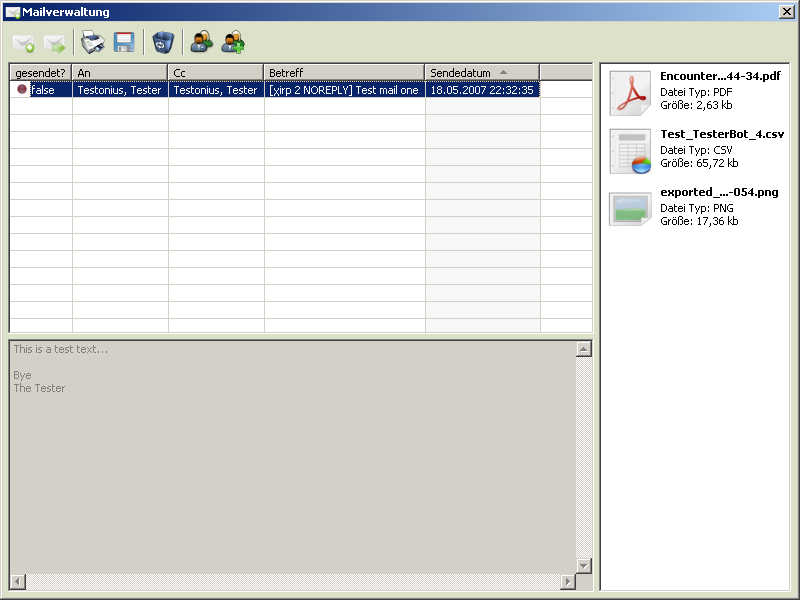
\includegraphics[width=.75\textwidth]{images/mailvw}
    \caption{Die Mailverwaltung}
    \label{img:mail:vw}
\end{figure}

\subsection{Bereiche der Mailverwaltung}
Die Mailverwaltung l�sst sich in vier Hauptbereiche aufteilen. Diese Bereiche
werden im folgenden genauer beschrieben.

\begin{itemize}
  \item Werkzeugleiste
  \item E-Mail Informationstabelle
  \item E-Mail Textbereich
  \item Liste der Anh�nge
\end{itemize}

\subsubsection{Werkzeugleiste}
Die Funktionen der Werkzeugleiste werden in Abschnitt \ref{ref:mail:functions}
ab Seite \pageref{ref:mail:functions} eingehend beschrieben.

\subsubsection{E-Mail Informationstabelle}
Die Informationstabelle - linke Seite, oberer Teil des Dialogs - enth�lt f�r jede
gespeicherte E-Mail einen Eintrag mit den wichtigsten Informationen �ber die
Mail. Die angebotenen Informationen sind:

\begin{itemize}
  \item Versendestatus
  \item Erster \enquote{An} Empf�ngername
  \item Erster \enquote{Cc} Empf�ngername
  \item Betreff
  \item Sendedatum
\end{itemize}

\paragraph{Versendestatus}
Der Versendestatus wird durch ein rotes oder ein gr�nes \seegls{Icon} signalisiert. Ein
rotes \seegls{Icon} zeigt an, dass die Mail (noch) nicht versendet werden konnte. Dies
kann z.B. im Fehlerfall passieren. Die Mail kann in einem solchen Fall dann mit
der \enquote{Weiterleiten} Funktion versendet werden. Ist das \seegls{Icon} gr�n wurde
die Mail versendet.

\paragraph{Erster \enquote{An} Empf�ngername}
Diese Tabellenspalte enth�lt den ersten Namen der Empf�ngerliste. Dies dient
der �bersicht\footnote{In Version 3.0.0 wird eine Funktion hinzukommen, die es
erlaubt die weiteren Empf�nger der Mail einzusehen}.

\paragraph{Erster \enquote{Cc} Empf�ngername}
Diese Tabellenspalte enth�lt den ersten Namen der \enquote{Carbon copy}
Empf�ngerliste. Dies dient der �bersicht\footnote{In Version 3.0.0 wird eine
Funktion hinzukommen, die es erlaubt die weiteren \enquote{Carbon copy}
Empf�nger der Mail einzusehen}.

\paragraph{Betreff}
Die Betreffzeile der Mail. Diese f�ngt immer mit \enquote{[\xirp~2 NOREPLY]} an,
um zum Einen anzuzeigen, dass diese E-Mail �ber \xirp~versendet wurde und zum
Anderen um zu zeigen, dass der Empf�nger nicht auf diese E-Mail antworten soll,
da eine Antwort nicht beim Absender ankommen w�rde, sondern an die spezifizierte
\enquote{no-reply} Adresse geleitet wird.

\paragraph{Sendedatum}
Das sekundengenaue Sendedatum der E-Mail.

\subsubsection{E-Mail Textbereich}
Wird eine E-Mail aus der Informationstabelle angeklickt, wird in diesem Bereich
der Text der E-Mail geladen. Der Text kann hier nur angesehen und nicht
ver�ndert werden.

\subsubsection{Liste der Anh�nge}
Wird eine E-Mail aus der Informationstabelle angeklickt, werden in diesem Bereich
Eintr�ge f�r jeden Anhang der Mail angezeigt. Jedes dieser Elemente informiert
�ber den Dateinamen, den Dateityp und die Gr��e der Datei. handelt es sich um
einen \xirp~bekannten Dateityp wird ein entsprechendes \seegls{Icon} angezeigt. Bekannte
Dateitypen sind:

\index{Mail!PDF}
\index{Mail!PNG}
\index{Mail!JPG}
\index{Mail!CSV}
\begin{itemize}
  \item PDF
  \item PNG
  \item JPG
  \item CSV
\end{itemize}

An eine Mail k�nnen nur Dateien der oben aufgez�hlten Dateitypen angeh�ngt
werden\footnote{An Version 3.0.0 wird es auch m�glich sein andere Dateitypen
anzuh�ngen}.

\subsection{Funktionen}
\label{ref:mail:functions}
In der Mailverwaltung stehen diverse Funktionen zur Verf�gung. Diese Funktionen
sind �ber die Werkzeugleiste verf�gbar. In Abbildung \ref{img:mail:vw:tools}
auf Seite \pageref{img:mail:vw:tools} ist die Werkzeugleiste als Ganzes zu sehen.
Die Funktionen der Werkzeugleiste sind von links nach rechts gesehen:

\begin{itemize}
  \item Neue Mail schreiben
  \item Mail weiterleiten
  \item Markierte Mails drucken
  \item Markierte Mails speichern
  \item Markierte Mails l�schen
  \item Kontaktpflege
  \item Neuen Kontakt anlegen
\end{itemize}

\begin{figure}[ht]
    \centering
    
\includegraphics[width=.75\textwidth]{images/mailsvwtools}
    \caption{Die Werkzeugleiste der Mailverwaltung}
    \label{img:mail:vw:tools}
\end{figure}

Im Tabelle \ref{tab:mailvwtools} auf Seite \pageref{tab:mailvwtools} werden die
Funktionen im einzelnen beschrieben.

\begin{table}[htp]
    \centering
    \begin{tabular}{c|l}
    Werkzeugelement & Beschreibung\\
    \hline
    
\includegraphics{images/send_mail} & Eine neue E-Mail schreiben/senden.\\
    
\includegraphics{images/forward_mail} & Eine markierte E-Mail weiterleiten.\\
    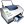
\includegraphics{images/print} & Eine markierte E-Mail drucken. Es werden der
    Text\\
    & der E-Mail und alle Anh�nge gedruckt.\\
    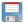
\includegraphics{images/save} & Eine markierte E-Mail speichern. Es wird
    unter\\
    & dem ausgew�hlten Ordner alle Anh�nge und der Text\\
    & der Mail abgelegt.\\
    
\includegraphics{images/delete} & Eine markierte E-Mail l�schen.\\
    
\includegraphics{images/contacts} & Die Kontaktverwaltung �ffnen.\\
    
\includegraphics{images/add_contact} & Einen neuen Kontakt anlegen\\
    \end{tabular}
    \caption{Die Elemente der Werkzeugliste der Mailverwaltung}
    \label{tab:mailvwtools}
    \index{Kontakte}
\end{table}

\section{Mailbearbeitung}
\index{Mail}
Der Dialog zum Bearbeiten/Weiterleiten von E-Mails ist in Abbildung
\ref{img:mail:edit} auf Seite \pageref{img:mail:edit} zu sehen. Der Dialog zum
Erstellen ist der Selbe, nur ohne vorausgef�llte Felder.

\begin{figure}[ht]
    \centering
    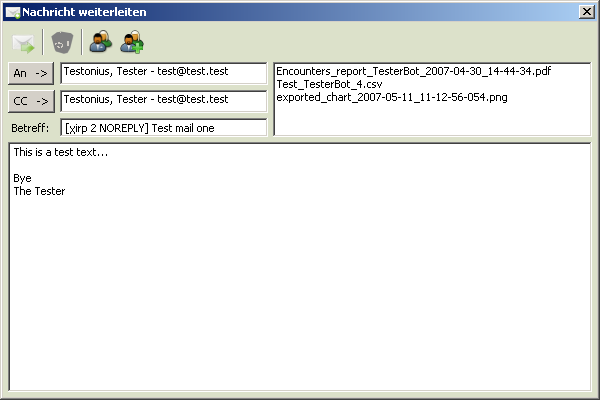
\includegraphics[width=.75\textwidth]{images/mailedit}
    \caption{Die Mailbearbeitung}
    \label{img:mail:edit}
\end{figure}

\subsection{Funktionen}
Es gibt vier Funktionen, die auch schon von der Mailverwaltung bekannt sind. Nur
die \enquote{L�schen} Funktion bezieht sich auf markierte Empf�nger und Anh�nge.
\par
Die Funktion zum Hinzuf�gen von Kontakten zu den \enquote{An}- und
\enquote{Cc}-Empf�ngerlisten kann �ber die Kn�pfe \texttt{An ->} und
\texttt{Cc ->} aufgerufen werden.
\par
Ist die E-Mail komplett zusammengestellt, d.h. wurde mindestens ein Empf�nger
angegeben, kann diese �ber das entsprechende \seegls{Icon} gesendet oder weitergeleitet
werden. Die entsprechenden \seegls{Icon}s werden �quivalent zu den Beschreibungen in
Tabelle \ref{tab:mailvwtools} auf Seite \pageref{tab:mailvwtools} benutzt.

\section{Kontaktverwaltung}
\index{Kontakte}
Die Kontaktverwaltung ist in Abbildung \ref{img:contact:vw} auf Seite
\ref{img:contact:vw} zu sehen. Auf der linken Seite befindet sich eine Liste mit
allen gespeicherten Kontakten. Jeder der Elemente der Liste stellt einen Kontakt
dar und informiert �ber Name, E-Mail Adresse und Telefonnummer des Kontaktes.
Das Geschlecht der Person des Kontaktes wird �ber drei Bilder angezeigt. Die
m�glichen Geschlechter sind \enquote{m�nnlich}, \enquote{weiblich} und
\enquote{undefiniert}.

\begin{figure}[ht]
    \centering
    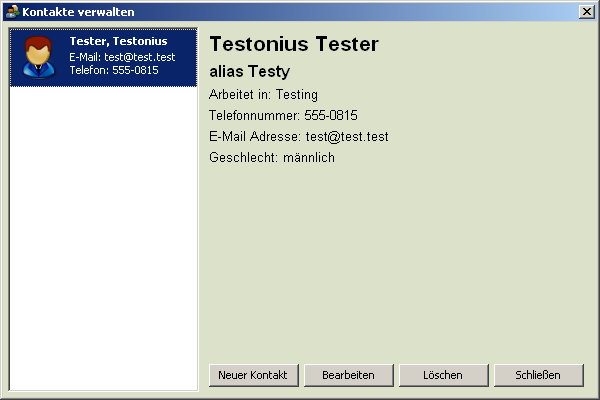
\includegraphics[width=.75\textwidth]{images/contactvw}
    \caption{Die Kontaktverwaltung}
    \label{img:contact:vw}
\end{figure}

Auf der rechten Seite befindet sich der Bereich in dem die kompletten
Informationen des momentan ausgew�hlten Kontaktes angezeigt werden. Am unteren
Rand des rechten Bereiches befinden sich vier Kn�pfe mit denen Funktionen
aufgerufen werden k�nnen.

\begin{itemize}
  \item \texttt{Neuer Kontakt}
  \item \texttt{Bearbeiten}
  \item \texttt{L�schen}
  \item \texttt{Schlie�en}
\end{itemize}

Die ersten beiden Funktionen beziehen sich auf das Erstellen und Bearbeiten von
Kontakten. Wie genau dies mittels der Kontaktbearbeitung geschieht, kann in
Abschnitt \ref{ref:mail:contact} ab Seite \pageref{ref:mail:contact} nachgelesen
werden. Die \enquote{L�schen}-Funktion entfernt den in der Liste der Kontakte
markierten Kontakt. Mit dem \texttt{Schlie�en}-Knopf wird die Kontaktverwaltung
geschlossen.

\newpage

\section{Kontaktbearbeitung}
\label{ref:mail:contact}
\index{Kontakte}
Der Eingabe-/Bearbeitungsdialog f�r Kontakte ist in Abbildung
\ref{img:mail:contact:edit} auf Seite \pageref{img:mail:contact:edit} zu sehen.

Es gibt sieben Angaben die f�r einen Kontakt gemacht werden k�nnen. Um den
Kontakt speichern zu k�nnen muss mindestens eine der Angaben gemacht werden.
Um E-Mails an den Kontakt versenden zu k�nnen muss nat�rlich einen E-Mail Adresse
angegeben werden.

\begin{itemize}
  \item Vorname
  \item Nachname
  \item Spitzname
  \item Abteilung
  \item Telefon \#
  \item E-Mail Adresse
  \item Geschlecht
\end{itemize}

\begin{figure}[ht]
    \centering
    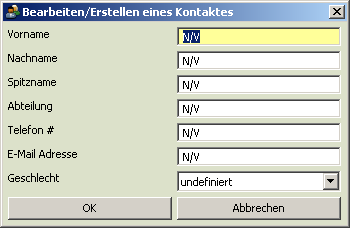
\includegraphics[width=.75\textwidth]{images/editcontact}
    \caption{Die Kontaktbearbeitung}
    \label{img:mail:contact:edit}
\end{figure}

\index{Mail|)}
\index{Kontakte|)}

\chapter{Diagramme und Aufzeichnungen}
\index{Auswertungen}
\index{Rekorder}
\index{Diagrammgenerator}
Das folgende Kapitel besch�ftigt sich mit den Auswertungs- und
Aufzeichnungsm�glichkeiten von \xirp. Mit Hilfe der in die Anwendung
integrierten Rekorder und Diagrammgeneratoren ergeben sich vielf�ltige
M�glichkeiten Werte, die vom Roboter geliefert werden, auszuwerten.
Die drei Hauptbereiche sind:

\begin{itemize}
  \item Live-Diagramme
  \item Aufzeichnungen
  \item Diagrammgenerator
\end{itemize}

\newpage

\section{Live-Diagramme}
\index{Live-Diagramme|(}
Jeder Roboterreiter enth�lt einige Standardbereiche. Zu diesen geh�rt auch der
Bereich der \enquote{Live-Diagramme}. Dieser ist in inaktiver Form in Abbildung
\ref{img:charts:livei} auf Seite \pageref{img:charts:livei} zu sehen.

\subsection{Konfiguration}
\index{Einstellungen}
Wie in Abschnitt \ref{ref:settings:livechart} ab Seite
\pageref{ref:settings:livechart} beschrieben, k�nnen mittels der Einstellungen
vier Exportvarianten festgelegt werden. Diese Dateien werden dann automatisch
beim Beenden des Vorgangs erstellt.
\par
\index{Live-Diagramme}
\index{Live-Diagramme!relative Zeit}
\index{Live-Diagramme!absolute Zeit}
\index{Live-Diagramme!Sensorschl�ssel}
Zum Konfigurieren des Live-Diagramms existieren im Live-Diagrammbereich zwei
Werkzeuge. In Abbildung \ref{img:charts:livei} auf Seite
\pageref{img:charts:livei} sind diese Werkzeuge farblich markiert. Das Men� zur
Auswahl von Sensorschl�sseln ist gr�n markiert. Hier k�nnen die zu beobachtenden
Sensorwerte ausgew�hlt werden. Mit dem rot markierten Knopf ist es m�glich die
Zeitleiste zwischen relativer (5min, 34sek) und absoluter (15:32:12 Uhr) Zeitangabe
umzuschalten. Ein rotes \enquote{A}
zeigt an, dass die absolute Zeit verwendet wird und ein rotes \enquote{R} zeigt
an, dass die relative Zeit verwendet wird.

\begin{figure}[ht]
    \centering
    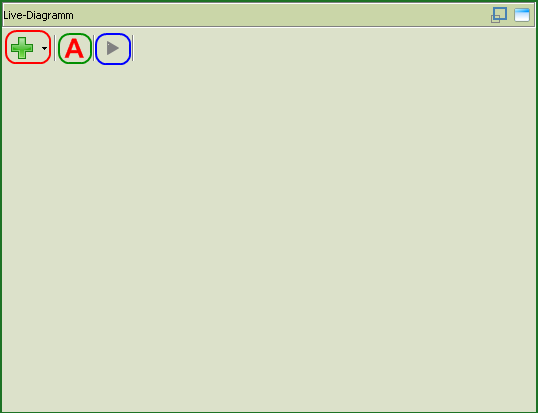
\includegraphics[width=.65\textwidth]{images/chartslivei}
    \caption{Der inaktive Live-Diagrammbereich}
    \label{img:charts:livei}
\end{figure}

\index{Live-Diagramme}
\index{Live-Diagramme!Sensorschl�ssel}
Um einen Live-Diagramm Vorgang zu starten, muss mindestens ein Sensorschl�ssel
des Roboters �ber das Men�, welches mit einem gr�nen Pluszeichen versehen ist,
ausgew�hlt werden. Dann kann mit dem blau markierten Startknopf der Vorgang
gestartet werden. Dieser Knopf wandelt sich dann in einen Stopknopf, mit dem der
Vorgang beendet werden kann. Sollte die Meldung \enquote{Keine Daten verf�gbar}
erscheinen, kann es sein dass der Schl�ssel nicht in der ben�tigten
Form\footnote{Dies kann ein Fehler im Protokoll-Plugin sein. Siehe hierzu das
entsprechende Kapitel im
\href{\devguideurl}{Developer Guide}.}
vorliegt, keine Verbindung zum Roboter besteht, oder der Roboter keine Werte
sendet.

\subsection{Benutzung}
\index{Live-Diagramme}
Wenn alle Einstellungen gemacht wurde, eine Verbindung zum Roboter besteht und
dieser Werte sendet, kann die Erstellung eines Live-Diagramms gestartet werden.
In Abbildung \ref{img:charts:livea} auf Seite \pageref{img:charts:livea} ist der
Live-Diagrammbereich w�hrend des Vorgangs zu sehen.

\begin{figure}[ht]
    \centering
    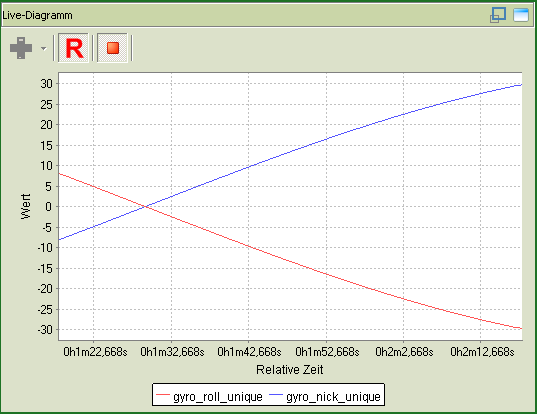
\includegraphics[width=.65\textwidth]{images/chartslivea}
    \caption{Der aktive Live-Diagrammbereich}
    \label{img:charts:livea}
\end{figure}

W�hrend des Vorgangs ist es nicht m�glich weitere Schl�ssel hinzuzuf�gen. Es ist
jedoch m�glich den Zeitmodus zwischen relativer und absoluter Zeit umzuschalten.
\index{Live-Diagramme|)}

\section{Aufzeichnungen}
\index{Aufzeichnungen|(}
\index{Rekorder|(}
In Abschnitt \ref{ref:charts:gen} wird die M�glichkeit beschrieben Diagramme auf
Grundlage von Aufzeichnungen zu Erstellen. Wie diese Aufzeichungen gemacht
werden k�nnen beschreibt dieser Abschnitt.
\par
\index{Live-Diagramm}
Wie auch schon bei den Live-Diagrammen existiert in jedem Roboterreiter ein
Bereich f�r Aufzeichnungen. Dieser Bereich ist in Abbildung
\ref{img:charts:recorder} auf Seite \pageref{img:charts:recorder}.

\begin{figure}[ht]
    \centering
    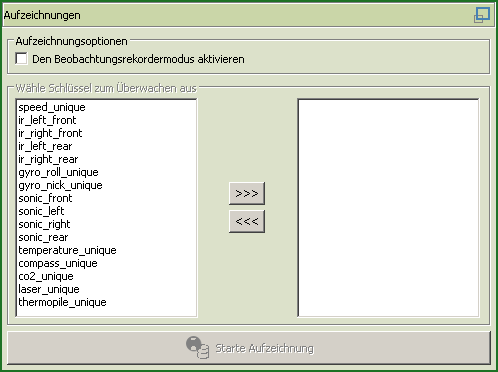
\includegraphics[width=.65\textwidth]{images/recorder}
    \caption{Der Aufzeichnungsrekorder}
    \label{img:charts:recorder}
\end{figure}

\index{Beobachtungsrekordermodus|(}
Der Rekorder hat Optionen zum Aktivieren verschiedener Rekordermodi\footnote{Ab
Version 3.0.0 ist geplant, dass nicht nur
ausgew�hlte Sensorwerte aufgezeichnet werden k�nnen, sondern auch die komplette
Kommunikation zwischen \xirp~und dem Roboter.}.

\begin{itemize}
  \item Beobachtungsrekordermodus
\end{itemize}

Der Beobachtungsrekordermodus wird in Abschnitt \ref{ref:charts:observed}
genauer beschrieben.

\subsection{Beobachtungsrekordermodus}
\label{ref:charts:observed}
\index{Rekorder}
\index{Sensorschl�ssel}
\index{Sensorschl�ssel!beobachtete}
Wenn die Option \enquote{Den Beobachtungsrekordermodus aktivieren} gesetzt ist,
k�nnen im unteren Bereich des Rekorders bestimmte Sensorschl�ssel markiert und
mittels des \texttt{>>>}-Knopfes zur Liste der beobachteten Schl�ssel
hinzugef�gt werden. Mittels des \texttt{<<<}-Knopfes k�nnen Schl�ssel aus der
Liste der zu beobachtenden Schl�ssel wieder entfernt werden. Dies funktioniert
nur, wenn die Aufzeichnung noch nicht l�uft. In Abbildung
\ref{img:charts:recorder2} auf Seite \pageref{img:charts:recorder2} ist zu
sehen, dass vier Schl�ssel zu der Liste der zu beobachtenden Schl�ssel
\index{Aufzeichnungen!starten}
hinzugef�gt wurden. Es ist ebenfalls zu sehen, dass der Knopf \enquote{Starte
Aufzeichnung} noch nicht benutzbar ist. Dies ist erst m�glich, wenn eine
Verbindung zum Roboter besteht.

\begin{figure}[ht]
    \centering
    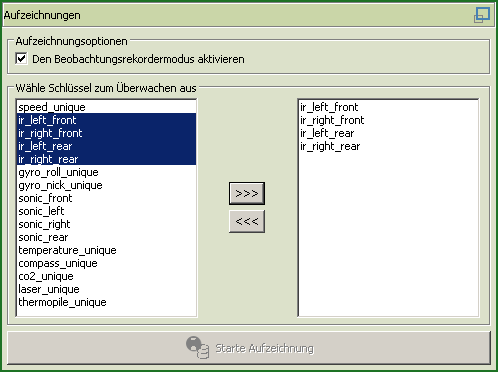
\includegraphics[width=.65\textwidth]{images/recorder2}
    \caption{Der Aufzeichnungsrekorder mit ausgew�hlten Schl�sseln}
    \label{img:charts:recorder2}
\end{figure}

\index{Aufzeichnungen!stoppen}
Wurde eine Verbindung zum Roboter hergestellt, kann die Aufzeichnung begonnen
werden. Wurde diese gestartet, verwandelt sich der \enquote{Starte
Aufzeichnung}-Knopf in einen \enquote{Stoppe Aufzeichnung}-Knopf.
Dieser Zustand des Rekorders ist in Abbildung \ref{img:charts:recorder3} auf
Seite \pageref{img:charts:recorder3} zu sehen.

\begin{figure}[ht]
    \centering
    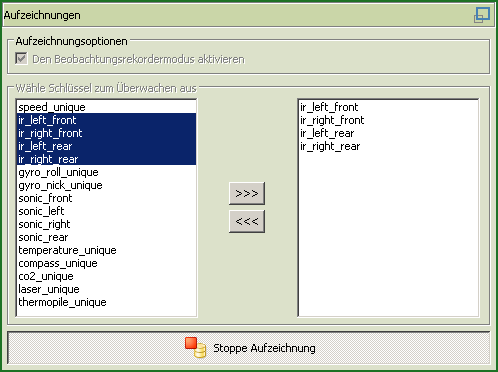
\includegraphics[width=.65\textwidth]{images/recorder3}
    \caption{Der Aufzeichnungsrekorder w�hred der Aufnahme}
    \label{img:charts:recorder3}
\end{figure}

Wird die Aufzeichnung durch Anklicken des Knopfes \enquote{Stoppe Aufzeichnung}
beendet, �ffnet sich ein Eingabedialog, in dem f�r die soeben beendete
Aufzeichnung ein Name und eine kurze Beschreibung eingegeben werden k�nnen. Die
Beschreibung ist optional, der Name jedoch verpflichtend. Hierdurch kann die
Wiedererkennbarkeit einer Aufzeichnung erh�ht werden, da ansonsten nur der
Aufzeichnungszeitraum die Aufzeichnung identifizieren kann.
\par
\index{Diagrammgenerator}
\index{Mail}
\index{Mail!CSV}
Die Aufzeichnungen werden in der Datenbank dauerhaft gespeichert und k�nnen �ber
das Mailsystem als \seegls{CSV}-Datei versendet, oder mittels des Diagrammgenerators in
graphischer Form ausgewertet werden.

\index{Beobachtungsrekordermodus|)}
\index{Aufzeichnungen|)}
\index{Rekorder|)}

\section{Diagrammgenerator}
\label{ref:charts:gen}
\index{Diagramme|(}
\index{Diagrammgenerator|(}
\index{Aufzeichnungen}
\index{Rekorder}
\index{Beobachtungsrekordermodus}
Mit Hilfe des Diagrammgenerators ist es m�glich Aufzeichnungen die mit dem
Rekorder im Beobachtungsrekordermodus gemacht wurden graphisch aufzuarbeiten und
als Diagramme anzeigen zu lassen. Hierbei werden zwei Modi der Generierung und
vier Diagrammtypen unterschieden. Diese Modi und Typen werden in den Abschnitten
\ref{ref:charts:modi} und \ref{ref:charts:types} genauer beschrieben.
Zun�chst soll zun�chst die Oberfl�che des Generators vorgestellt werden.

\subsection{Die Generatoroberfl�che}
Der Diagrammgenerator direkt nach seinem Aufruf ist in Abbildung
\ref{img:charts:gen} auf Seite \pageref{img:charts:gen} zu sehen.

\begin{figure}[ht]
    \centering
    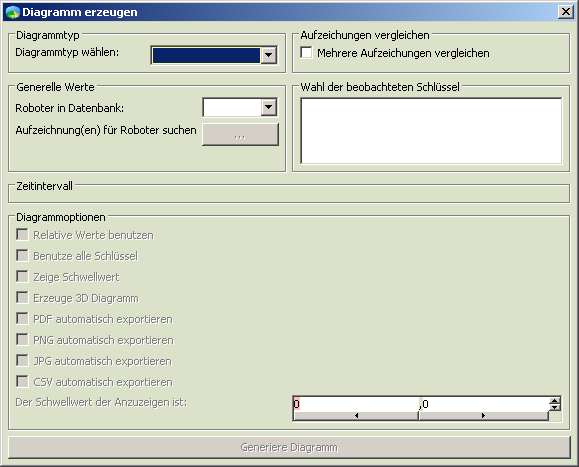
\includegraphics[width=.75\textwidth]{images/chartgen}
    \caption{Der Diagrammgenerator}
    \label{img:charts:gen}
\end{figure}

In den im folgenden aufgez�hlten Bereichen k�nnen verschiedenste Einstellungen
vorgenommen werden. Diese Einstellungen beeinflussen die Art und Weise der
Erstellung und das Erscheinungsbild des Diagramms.

\begin{itemize}
  \item Diagrammtyp
  \item Aufzeichnungen vergleichen
  \item Generelle Werte
  \item Wahl der beobachteten Schl�ssel
  \item Zeitintervall
  \item Diagrammoptionen
\end{itemize}

\subsubsection{Diagrammtyp}
Hier wird der Typ des zu Erstellenden Diagramms ausgew�hlt. Mehr �ber die
verschiedenen Typen kann in Abschnitt \ref{ref:charts:types} ab Seite
\pageref{ref:charts:types} nachgelesen werden.

\subsubsection{Aufzeichnungen vergleichen}
Hier wird entschieden, welcher Modus des Generators benutzt werden soll. Wird
die Option \enquote{Mehrere Aufzeichnungen vergleichen} aktiviert, ist es m�glich
in der Aufzeichnungsauswahl bis zu vier Aufzeichnungen auszuw�hlen. Die
Auszeichnungen werden dann in dem resultierenden Diagramm gegen�bergestellt.

\subsubsection{Generelle Werte}
Hier muss zuerst der Roboter ausgew�hlt werden, f�r den Aufzeichnungen
vorliegen. Danach kann mittels des Knopfes \enquote{\texttt{\ldots}} der
Auswahldialog f�r Aufzeichnungen aufgerufen werden. Ist die Option
\enquote{Mehrere Aufzeichnungen vergleichen} aktiviert, k�nnen hier bis zu vier
Aufzeichnungen ausgew�hlt werden. Ist die Option nicht aktiv kann nur eine
Aufzeichnung gew�hlt werden.

\subsubsection{Wahl der beobachteten Schl�ssel}
\index{Sensorschl�ssel}
Wurden eine oder mehrere Aufzeichnungen ausgew�hlt, werden in der Liste dieses
Bereiches die Sensorschl�ssel der Aufzeichnung angezeigt. Wenn mehrere
Aufzeichnungen ausgew�hlt wurde, werden nur die Schl�ssel angezeigt die in allen
Aufzeichnungen vorhanden sind, da diese ja verglichen werden sollen.
\par
Um ein Diagramm zu erstellen, muss in der Liste der beobachteten Sensorschl�ssel
mindestens ein Eintrag markiert werden. Die Werte der markierten Schl�ssel
werden bei der Erstellung des Diagramm mit einbezogen.

\subsubsection{Zeitintervall}
Hier kann mittels der Schieberegler der Zeitintervall bestimmt werden, �ber den
die beobachteten Werte in das Diagramm einbezogen werden sollen. Auch hier gibt
es zwei Varianten, bestimmt durch die \enquote{Mehrere Aufzeichnungen
vergleichen} Option. Der oder die Schieberegler erscheinen, wenn ein oder
mehrere Aufzeichnungen ausgew�hlt wurden.

\paragraph{\enquote{Mehrere Aufzeichnungen vergleichen} aktiv}
\index{Diagrammgenerator!Zeitintervallauswahl}
In Abbildung \ref{img:charts:gen:interval:single} auf Seite
\pageref{img:charts:gen:interval:single} ist die Zeitintervallauswahl f�r eine
einzelne ausgew�hlte Aufzeichnung zu sehen.
\par
Mittels der zwei Schieberegler l�sst sich ein Intervall innerhalb des Zeitraumes
der Aufzeichnung einstellen. Dieser Bereich wird dann bei der Generierung des
Diagramms betrachtet.

\begin{figure}[ht]
    \centering
    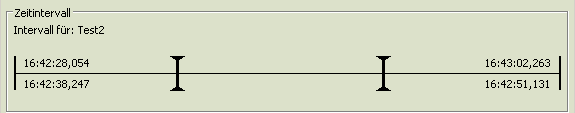
\includegraphics[width=.75\textwidth]{images/interval_single}
    \caption{Die Zeitintervallauswahl f�r eine einzelne Aufzeichnung}
    \label{img:charts:gen:interval:single}
\end{figure}

\paragraph{\enquote{Mehrere Aufzeichnungen vergleichen} nicht aktiv}
\index{Diagrammgenerator!Zeitintervallauswahl}
In Abbildung \ref{img:charts:gen:interval:multi} auf Seite
\pageref{img:charts:gen:interval:multi} ist die Zeitintervallauswahl f�r vier
ausgew�hlte Aufzeichnungen zu sehen.
\par
Zus�tzlich zu den vier Intervallreglern gibt es in diesem Modus ein Eingabefeld,
um den Zeitintervall in Millisekunden festzulegen. Dies ist n�tig, da die
Aufzeichnungen unterschiedlich lang sein k�nnen und um immer den gleichen
Zeitintervall vergleichen zu k�nnen. Das Maximum des Intervalls ist die
komplette Dauer der k�rzesten Aufzeichnung. Die Regler der Zeitintervallauswahl
k�nnen nun nicht mehr einzeln bewegt werden, sondern bleiben immer in dem
eingestellten Abstand.

\begin{figure}[ht]
    \centering
    \includegraphics[width=.75\textwidth]{images/interval_multi}
    \caption{Die Zeitintervallauswahl f�r mehrere Aufzeichnungen}
    \label{img:charts:gen:interval:multi}
\end{figure}

\subsubsection{Diagrammoptionen}
In diesem Bereich gibt es neun Optionen die aktiviert werden k�nnen. Nicht jede
Option ist f�r jeden Diagrammtyp verf�gbar und einige Optionen haben, f�r einen
Diagrammtyp, unterschiedliche Auswirkungen auf das generierte Diagramm.

\paragraph{Relative Werte benutzen}
Bei den Diagrammtypen \enquote{Zeitdiagramm}, \enquote{Balkendiagramm} und
\enquote{Punktdiagramm} wird die die Zeitachse mit relativen Werten (5min, 54sek)
versehen. Beim Typ \enquote{Tortendiagramm} werden prozentuale Angaben der
Schl�ssel verwendet. Eine weitere Besonderheit dieser Option beim Tortendiagramm
ist der Effekt, dass die Option \enquote{Alle Schl�ssel benutzen} aktiviert
wird, wenn diese Option f�r ein Tortendiagramm aktiviert wird.

\paragraph{Benutze alle Schl�ssel}
Wird diese Option aktiviert, werden alle in der Liste der beobachteten Schl�ssel
vorhandenen Eintr�ge bei der Erstellung des Diagramms ber�cksichtigt.

\newpage

\paragraph{Zeige Schwellwert}
Wird diese Option aktiviert, kann mittels des Eingabefeldes \enquote{Der
Schwellwert der Anzuzeigen ist} ein Schwellwert eingegeben werden, der dann
mittels einer orangenen Linie im generierten Diagramm angezeigt wird.
\par
Diese Option ist \textbf{nicht} f�r das Tortendiagramm verf�gbar.

\paragraph{Erzeuge 3D Diagramm}
Wird diese Option aktiviert, wird eine \enquote{3D} Version des Diagramms
erzeugt.
\par
Diese Option ist \textbf{nur} f�r das Tortendiagramm verf�gbar.

\paragraph{PDF automatisch exportieren}
\index{Diagramme!Export!PDF}
Wird diese Option aktiviert, wird das generierte Diagramm automatisch nach der
Erstellung als \seegls{PDF}-Datei exportiert. Die Datei wird in der folgenden
Ordnerstruktur abgelegt.
\par
\begin{center}
\texttt{<xirp>/charts/<robotername>/pdf}
\end{center}
\par
Die Option ist f�r \textbf{alle} Diagrammtypen verf�gbar.

\paragraph{PNG automatisch exportieren}
\index{Diagramme!Export!PNG}
Wird diese Option aktiviert, wird das generierte Diagramm automatisch nach der
Erstellung als PNG-Datei exportiert. Die Datei wird in der folgenden
Ordnerstruktur abgelegt.
\par
\begin{center}
\texttt{<xirp>/charts/<robotername>/png}
\end{center}
\par
Die Option ist f�r \textbf{alle} Diagrammtypen verf�gbar.

\paragraph{JPG automatisch exportieren}
\index{Diagramme!Export!JPG}
Wird diese Option aktiviert, wird das generierte Diagramm automatisch nach der
Erstellung als JPG-Datei exportiert. Die Datei wird in der folgenden
Ordnerstruktur abgelegt.
\par
\begin{center}
\texttt{<xirp>/charts/<robotername>/jpg}
\end{center}
\par
Die Option ist f�r \textbf{alle} Diagrammtypen verf�gbar.

\paragraph{CSV automatisch exportieren}
\index{Diagramme!Export!CSV}
Wird diese Option aktiviert, wird das generierte Diagramm automatisch nach der
Erstellung als \seegls{CSV}-Datei exportiert. Die Datei wird in der folgenden
Ordnerstruktur abgelegt.
\par
\begin{center}
\texttt{<xirp>/charts/<robotername>/csv}
\end{center}
\par
Die Option ist f�r \textbf{alle} Diagrammtypen verf�gbar.

\subsection{Modi der Diagrammgenerierung}
\label{ref:charts:modi}
Wie bereits erw�hnt, gibt es zwei Modi der Diagrammgenerierung:

\begin{itemize}
  \item Einfaches Diagramm
  \item Vergleich mehrerer Aufzeichnungen
\end{itemize}

Diese Modi werden in den folgenden Abschnitten genauer beschrieben.

\subsubsection{Einfaches Diagramm}
\index{Diagramme!Diagrammansicht}
Wird die Option \enquote{Mehrere Aufzeichnungen vergleichen} nicht aktiviert,
kann nur eine einzelne Aufzeichnung ausgew�hlt werden. Wird das Diagramm mittels
des Knopfes \enquote{Generiere Diagramm} erzeugt, �ffnet sich die
Diagrammansicht mit einem einzelnen Diagramm. Ein Beispiel hierf�r ist in
Abbildung \ref{img:chart:single} auf Seite \pageref{img:chart:single} zu sehen.

\begin{figure}[ht]
    \centering
    \includegraphics[width=.8\textwidth]{images/single_chart}
    \caption{Ein einfaches Diagramm in der Diagrammansicht}
    \label{img:chart:single}
\end{figure}

\subsubsection{Vergleich mehrerer Aufzeichnungen}
\index{Diagramme!Diagrammansicht}
Wird die Option \enquote{Mehrere Aufzeichnungen vergleichen} aktiviert, k�nnen
bis zu vier Aufzeichnungen ausgew�hlt und verglichen werden. Die Liste der
beobachteten Schl�ssel enth�lt nur jene Schl�ssel, die in jeder Aufzeichnung
vorkommen. Wird das Diagramm mittels des Knopfes \enquote{Generiere Diagramm}
erzeugt, �ffnet sich die Diagrammansicht mit je einem Diagramm f�r jede gew�hlte
Aufzeichnung. Ein Beispiel mit vier Aufzeichnungen ist in Abbildung
\ref{img:chart:multi} auf Seite \pageref{img:chart:multi} zu sehen.

\begin{figure}[ht]
    \centering
    \includegraphics[width=1\textwidth]{images/chart_multi}
    \caption{Vier Diagramme in der Diagrammansicht}
    \label{img:chart:multi}
\end{figure}

\subsection{Diagrammtypen}
\label{ref:charts:types}
Wie bereits erw�hnt gibt es die folgenden vier verschiedenen Diagrammtypen.

\begin{itemize}
  \item Zeitdiagramm
  \item Tortendiagramm
  \item Balkendiagramm
  \item Punktdiagramm
\end{itemize}

Die Diagrammypen werden in den folgenden Abschnitten einzeln beschrieben.

\subsubsection{Zeitdiagramm}
Dieser Diagrammtyp zeigt die Entwicklung eines Wertes �ber einen gewissen
Zeitraum. Es kann ein Schwellwert angezeigt werden. Mehrere Sensorwerte k�nnen
so verglichen werden. Ein Beispiel in in Abbildung
\ref{img:chart:export:png:time} auf Seite \pageref{img:chart:export:png:time}
zu sehen. Dieses Beispiel zeigt gleichzeitig, wie das generierte Diagramm als
exportierte PNG-Datei aussieht.

\begin{figure}[ht]
    \centering
    \includegraphics[width=.5\textwidth]{images/exported_chart_2007-06-20_19-37-33-850}
    \caption{Ein als PNG-Datei exportiertes Zeitdiagramm}
    \label{img:chart:export:png:time}
\end{figure}

\subsubsection{Tortendiagramm}
Dieser Diagrammtyp kann verwendet werden, um das Vorkommen von bestimmten
Sensorwerten total oder prozentual auszuwerten. Im Beispiel in Abbildung
\ref{img:chart:export:png:pie} auf Seite \pageref{img:chart:export:png:pie}
werden die Vorkommen von sechs Sensorwerten prozentual\footnote{Im Beispiel
herrscht eine Gleichverteilung der Werte, dies muss in der realen Welt nicht so
sein.} angegeben.

\begin{figure}[ht]
    \centering
    \includegraphics[width=.5\textwidth]{images/exported_chart_2007-06-20_20-09-31-167}
    \caption{Ein als PNG-Datei exportiertes Tortendiagramm}
    \label{img:chart:export:png:pie}
\end{figure}

\subsubsection{Balkendiagramm}
Dieser Diagrammtyp zeigt die Entwicklung von Sensorwerten �ber einen bestimmten
Zeitraum in Balkenform. Sensorwerte k�nnen so verglichen werden. In Abbildung
\ref{img:chart:export:png:bar} auf Seite \pageref{img:chart:export:png:bar}
befindet sich ein Beispiel f�r ein Balkendiagramm.

\begin{figure}[ht]
    \centering
    \includegraphics[width=.5\textwidth]{images/exported_chart_2007-06-20_20-19-23-889}
    \caption{Ein als PNG-Datei exportiertes Balkendiagramm}
    \label{img:chart:export:png:bar}
\end{figure}

\subsubsection{Punktdiagramm}
Dieser Diagrammtyp zeichnet f�r jeden Wert einen Punkt. Besonders gut geeignet
ist dieser Diagrammtyp f�r Werte die gro�e Spr�nge aufweisen. In Abbildung
\ref{img:chart:export:png:scatter} auf Seite
\pageref{img:chart:export:png:scatter} befindet sich ein Beispiel f�r ein
Punktdiagramm.

\begin{figure}[ht]
    \centering
    \includegraphics[width=.5\textwidth]{images/exported_chart_2007-06-20_20-24-03-642}
    \caption{Ein als PNG-Datei exportiertes Punktdiagramm}
    \label{img:chart:export:png:scatter}
\end{figure}

\newpage

\subsection{Diagrammansicht}
\index{Diagramme!Diagrammansicht}
Jedes generierte Diagramm wird in einem neuen Fenster ge�ffnet: Der
Diagrammansicht. Die Diagrammansicht hat einige weitere Funktionen die der
Benutzer aufrufen kann.

\begin{itemize}
  \item Zoomen mit der Maus
  \item Zoomen mittels des Kontextmen�s
  \item Exportieren des Diagramms
\end{itemize}

Diese Funktionen werden in den folgenden Abschnitten genauer betrachtet. Die
Diagrammansicht war bereits in Abbildung \ref{img:chart:single} auf Seite
\pageref{img:chart:single} zu sehen.

\subsubsection{Zoomen mit der Maus}
\label{ref:charts:zoom}
\index{Diagramme!Diagrammansicht!hereinzoomen}
Es ist m�glich in das Diagramm hineinzuzoomen, indem mit der Maus ein Bereich
markiert wird. Hierzu muss die linke Maustaste gedr�ckt werden und der Bereich
von links oben nach rechts unten gezogen werden. Wird die Maustaste losgelassen
wird er neue Zoomstatus hergestellt.
\par
\index{Diagramme!Diagrammansicht!herauszoomen}
Um den Originalstatus wiederherzustellen, kann mit der Maus wieder
herausgezoomt werden. Hierzu muss die linke Maustaste gedr�ckt und von rechts
unten nach links oben bewegt werden. Wird die Maustaste losgelassen
wird er neue Zoomstatus hergestellt.

\subsubsection{Zoomen mittels des Kontextmen�s}
Die in Abschnitt \ref{ref:charts:zoom} beschriebenen Zoomfunktionen sind auch
�ber ein Kontextmen� verf�gbar. Dieses Men� kann durch einen Klick der rechten
Maustaste aufgerufen werden. F�r hereinzoomen und herauszoomen existieren
gleichnamige Eintr�ge. Es kann zwischen den einzelnen Achsen, oder der
M�glichkeit beide Achsen zu Zoomen gew�hlt werden. Der neue Zoomstatus wird
sofort nach dem Anklicken der gew�nschten Funktion hergestellt.

\begin{itemize}
  \item Hereinzoomen
    \begin{itemize}
        \item Alle Achsen
        \item Abzisse (x-Achse)
        \item Ordinate (y-Achse)
    \end{itemize}
  \item Herauszoomen
    \begin{itemize}
        \item Alle Achsen
        \item Abzisse (x-Achse)
        \item Ordinate (y-Achse)
    \end{itemize}
\end{itemize}

\newpage

\subsubsection{Exportieren des Diagramms}
Das Kontextmen�, welches mittels der rechten Maustaste aufgerufen werden kann,
enth�lt zus�tzlich zu Zoomfunktionen drei Exportfunktionen. Das Diagramm wird in
der Form exportiert, in der es sich zu dem Exportmoment befindet. So kann auch
ein gezoomter Zustand gespeichert werden.

\begin{itemize}
  \item PDF exportieren
  \item PNG exportieren
  \item JPG exportieren
\end{itemize}

Die erzeugten Dateien werden wie gewohnt in der folgenden Ordnerstruktur
gespeichert.

\begin{center}
    \texttt{<xirp>/charts/<robotername>/pdf}\\
    \texttt{<xirp>/charts/<robotername>/png}\\
    \texttt{<xirp>/charts/<robotername>/jpg}\\
\end{center}

\index{Diagrammgenerator|)}
\index{Diagramme|)}

\chapter{Testerbot}
\index{Testerbot|(}

Dieses Kapitel befasst sich mit dem in \xirp~vorhandenen \seegls{Testerbot} \seegls{Server}.
Dieser \seegls{Server} erzeugt f�r verschiedenste \seegls{Sensor}en Zufallswerte und sendet sie an
den verbundenen \seegls{Client}. Dadurch ist es m�glich neue Plugins zu Testen. Der
\seegls{Testerbot} kann auch dazu verwendet werden, die Anwendung zu demonstieren, ohne
dass eine aufw�ndige Roboter-Simulation oder ein echter Roboter benutzt werden m�ssen.

\newpage

\section{Kontrolloberfl�che}
\index{Testerbot!Kontrolloberfl�che}
Der \seegls{Testerbot} \seegls{Server} kann bequem aus der Anwendung heraus gestartet werden. �ber
den Men�eintrag \texttt{Extras --> Testerbot ausf�hren} wird die
Kontrolloberfl�che aufgerufen. Diese Oberfl�che ist in Abbildung
\ref{img:testerbot:control:off} auf Seite \pageref{img:testerbot:control:off} zu
sehen.

\begin{figure}[ht]
    \centering
    \includegraphics[width=.75\textwidth]{images/tbserverctrl}
    \caption{Die Testerbot Kontrolloberfl�che - Server abgeschaltet.}
    \label{img:testerbot:control:off}
\end{figure}

Die Kontrolloberfl�che ist in drei Bereiche aufgeteilt.

\begin{itemize}
  \item Serverinformationen
  \item Servereinstellungen
  \item Serverkontrolle
\end{itemize}

Die einzelnen Bereiche werden in den folgenden Abschnitten genauer beschrieben.
In Abbildung \ref{img:testerbot:control:on} auf Seite
\pageref{img:testerbot:control:on} ist die Oberfl�che mit aktiviertem \seegls{Server} zu
sehen.

\begin{figure}[ht]
    \centering
    \includegraphics[width=.75\textwidth]{images/tbserverctrl_an}
    \caption{Die Testerbot Kontrolloberfl�che - Server angeschaltet.}
    \label{img:testerbot:control:on}
\end{figure}

\newpage

\subsection{Serverinformationen}
\index{Testerbot!Kontrolloberfl�che!Serverinformationen}
In diesem Bereich werden die folgenden Informationen �ber den \seegls{Server} angezeigt.

\begin{itemize}
  \item Serverstatus (An oder Aus)
  \item Anzahl verbundener Clients
  \item Gesendete Pakete
  \item Gesendete Datenmenge
\end{itemize}

\subsection{Servereinstellungen}
\index{Testerbot!Kontrolloberfl�che!Servereinstellungen}
Die einzige Einstellung die in der Oberfl�che gemacht werden kann ist die
Einstellung des Serverports. Der Standardwert ist \texttt{2005}. Ein neuer Wert
wird bei einem Neustart des \seegls{Server} benutzt.

\subsection{Serverkontrolle}
\index{Testerbot!Kontrolloberfl�che!Serverkontrolle}
In diesen Bereich gibt es zwei Kn�pfe. Nur jeweils einer ist aktiv. Die
Bezeichnung der Kn�pfe spricht f�r sich selbst und seine Funktion.

\begin{itemize}
  \item Starte Server
  \item Stoppe Server
\end{itemize}

Wird die Kontrolloberfl�che geschlossen, wird auch automatisch der \seegls{Server}
beendet. Daher muss die Oberfl�che immer angezeigt werden, wenn der \seegls{Server}
laufen soll. Die Oberfl�che kann allerdings minimiert werden.

\section{Gesendete Werte}
Der \seegls{Server} sendet Werte f�r diverse \seegls{Sensor}en. Die unterst�tzten \seegls{Sensor}en werden
im folgenden beschrieben.

\subsection{Energiequelle}
Es werden Werte f�r zwei Energiequellen gesendet.

\subsection{Infrarot}
Es werden Werte f�r vier Infrarotabstandssensoren gesendet.

\subsection{Ultraschall}
Es werden Werte f�r vier Untraschallabstandssensoren geliefert.

\subsection{Temperatur}
Es wird ein Temperaturwert gesendet.

\subsection{Thermopile}
\index{Live-Diagramm}
\index{Aufzeichungen}
Es wird ein Termopile-Array Scan geliefert. Dieser Scan besteht aus 32 mal 8
Werten. Daher ist dieser \seegls{Sensor} nicht f�r Aufzeichungen und Live-Diagramm
verwendbar.

\subsection{CO$_2$}
Es wird ein Kohlendioxidwert geliefert.

\subsection{Kompass}
Es wird ein Himmelsrichtungswert gesendet.

\subsection{Geschwindigkeit}
Es wird ein Geschwindigkeitswert gesendet.

\subsection{Neigung}
Es werden zwei Werte f�r die horizontale und vertikale Neigung geliefert.

\subsection{Laserscanner}
\index{Live-Diagramm}
\index{Aufzeichungen}
Es wird ein \seegls{Laserscanner} Scan geliefert. Dieser Scan besteht aus mehr als 600
einzelnen Werten, so dass dieser \seegls{Sensor} nicht f�r Aufzeichungen und Live-Diagramm
verwendbar ist.

\subsection{Nachrichten}
Es werden diverse Zufallstextnachrichten vom \seegls{Server} gesendet. Diese k�nnen z.B.
zum Testen der Sprachausgabe benutzt werden.

\index{Testerbot|)}

\chapter{Standard-Plugins}
\index{Plugins|(}
\index{Testerbot}
Die Installation von \xirp~enth�lt die n�tigen Profildateien f�r den
\seegls{Testerbot}. Ebenfalls werden einige Plugins mitgeliefert, die f�r den \seegls{Testerbot}
ben�tigt werden. In diesem Kapitel werden diese Plugins vorgestellt und n�her
beschrieben. Des Weiteren werden einige Kommunikationsplugins mitgeliefert, z.B.
ein Plugin f�r Kommunikation �ber die serielle Schnittstelle.

\newpage

\section{Hallo Welt!}
Das \enquote{Hallo Welt!} Plugin ist das erste Plugin, dass je f�r
\xirp~entwickelt wurde. In seiner momentanen Version ist dieses Plugin
ohne graphische Oberfl�che. Es wird mittels seines Men�eintrages \texttt{Plugins
--> Hallo Welt!} gestartet und gibt in der Systemprotokollansicht einen in den
Einstellungen �nderbaren Text an. Der Standardtext ist \enquote{Hallo Welt!}.
Diese Funktion kann ebenfalls mit dem vom Plugin erzeugten Werkzeugicon
aufgerufen werden. Das \seegls{Icon} ist gekennzeichnet durch ein Puzzelteilbild.

\section{Testerbot Report}
Dieses Plugin zeigt die Funktionsweise von Report-Plugins. Es erzeugt, bei Aufruf
�ber den entsprechenden Men�eintrag (\texttt{Reporte --> Testerbot Report}),
einen Report der die �bertragenen Textnachrichten darstellt.

\section{Thermopile}
\index{Thermopile}
\index{Temperatur}
Dieses \seegls{Sensor}-Plugin zeigt die von einem \seegls{Thermopile}-Array gelieferten W�rmewerte
an. Es zeigt die gemessene Temperatur farblich markiert an. Eine
Farb-Temperaturskala ist unter dem Anzeigebereich angezeigt. In Abbildung
\ref{img:plugins:thermo} auf Seite \pageref{img:plugins:thermo} ist das Plugin in
Aktion zu sehen.

\begin{figure}[ht]
	\centering
	\includegraphics[width=.75\textwidth]{images/thermo}
	\caption{Das Thermopile-Array-Plugin}
	\label{img:plugins:thermo}
\end{figure}

\section{Distanz}
\index{Abstandssensor}
\index{Roboterprofil}
Dieses Plugin zeigt die Werte von Abstandssensoren an. Dieses Plugin bezieht die
Informationen �ber Anzahl und Wertebereich der \seegls{Sensor}en aus dem Roboterprofil. 
In Abbildung \ref{img:plugins:distanz} auf Seite \pageref{img:plugins:distanz}
ist das Plugin in Aktion zu sehen.

\begin{figure}[ht]
	\centering
	\includegraphics[width=.4\textwidth]{images/distanz}
	\caption{Das Distanz-Plugin}
	\label{img:plugins:distanz}
\end{figure}

\index{Abstandssensor!Infrarot}
\index{Abstandssensor!Ultraschall}
\index{Roboterprofil}
Infratorsensoren werden farblich anders dargestellt als Ultraschallsensoren.
Infratorsensoren werden gr�n und Ultraschallsensoren blau dargestellt, wenn der
Entfernungswert gr��er oder gleich dem Maximum des \seegls{Sensor}s entspricht. Die Farbe
der Sensoranzeigen variiert mit den sich ver�ndernden Werten. Die Einheit in der
die Werte angezeigt werden, werden ebenfalls aus dem Roboterprofil ausgelesen.

\section{Temperatur}
\index{Temperatur}
\index{Thermometer}
\index{Roboterprofil}
Das Temperatur-Plugin zeigt die Werte eines W�rmesensors in Form eines
Thermometers an. Die Markierungen f�r den gelben und roten Bereich erh�lt das
Plugin aus dem Roboterprofil. Die Einheit in der der Wert angezeigt wird, wird
ebenfalls aus dem Roboterprofil ausgelesen. In Abbildung
\ref{img:plugins:temperatur} auf Seite
\pageref{img:plugins:temperatur} ist das Plugin in Aktion zu sehen.

\begin{figure}[htp]
	\centering
	\includegraphics[width=.2\textwidth]{images/temperatur}
	\caption{Das Temperatur-Plugin}
	\label{img:plugins:temperatur}
\end{figure}

\section{CO$_2$}
\index{Kohlendioxid}
\index{CO$_2$}
Dieses \seegls{Sensor}-Plugin zeigt den Verlauf der Werte eines CO$_2$-Sensors an, um so
einen Anstieg des Gases in der umgebenen Luft erkennen zu k�nnen. In Abbildung
\ref{img:plugins:co2} auf Seite \pageref{img:plugins:co2} ist das Plugin in
Aktion zu sehen.

\begin{figure}[ht]
	\centering
	\includegraphics[width=.6\textwidth]{images/co2}
	\caption{Das CO$_2$-Plugin}
	\label{img:plugins:co2}
\end{figure}

\section{Kompass}
\index{Kompass}
\index{Himmelsrichtung}
Das Kompass-Plugin zeigt die aktuell gemessene Himmelsrichtung eines
Kompasssensors in Form eines Kompasses an. Die rote Nadelspitze zeigt die
gemessene Richtung an. In Abbildung \ref{img:plugins:kompass} auf Seite
\pageref{img:plugins:kompass} ist das Plugin in Aktion zu sehen.

\begin{figure}[ht]
	\centering
	\includegraphics[width=.4\textwidth]{images/kompass}
	\caption{Das Kompass-Plugin}
	\label{img:plugins:kompass}
\end{figure}

\section{Geschwindigkeit}
\index{Geschwindigkeit}
\index{Tachometer}
Dieses Plugin zeigt die gemessene Geschwindigkeit eines Roboters in Form eines
Tachometers an. Die Einheit in der der Wert angezeigt wird, wird
aus dem Roboterprofil ausgelesen. In Abbildung \ref{img:plugins:speed} auf Seite
\pageref{img:plugins:speed} ist das Plugin in Aktion zu sehen.

\begin{figure}[htp]
	\centering
	\includegraphics[width=.4\textwidth]{images/speed}
	\caption{Das Geschwindigkeits-Plugin}
	\label{img:plugins:speed}
\end{figure}

\section{Neigung}
\index{Neigung}
\index{Gyroskop}
Dieses Plugin zeigt die gemessenen Werte eines Gyroskops an. Es werden zwei
Werte, die horizontale und die vertikale Neigung, angezeigt. Die Form der
Anzeige ist dem k�nstlichen Horizont, bekannt aus der modernen Avionik,
nachempfunden. Der \enquote{Himmel} ist blau und die \enquote{Erde} gr�n
gef�rbt. In Abbildung \ref{img:plugins:neigung} auf Seite
\pageref{img:plugins:neigung} ist das Plugin in Aktion zu sehen.

\begin{figure}[htp]
	\centering
	\includegraphics[width=.4\textwidth]{images/neigung}
	\caption{Das Neigungs-Plugin}
	\label{img:plugins:neigung}
\end{figure}

\section{Laserentfernungsmesser}
\index{Laserentfernungsmesser}
Dieses Plugin zeigt Scans eines Laserscaners an. Aus einem solchen Scan
resultiert eine grober Umriss der Umgebung. Die F�llfarbe kann gew�hlt werden.
Eine weitere Option ist, einen Rand um den Umriss zeichnen zu lassen. In
Abbildung \ref{img:plugins:laser} auf Seite \pageref{img:plugins:laser} ist das
Plugin in Aktion zu sehen.

\begin{figure}[htp]
	\centering
	\includegraphics[width=.4\textwidth]{images/laser}
	\caption{Das Laserentfernungsmesser-Plugin}
	\label{img:plugins:laser}
\end{figure}

\section{Nachrichten}
\index{Testerbot}
\index{Sprachausgabe}
\index{Kommandos}
Das Nachrichten-Plugin zeigt die vom \seegls{Testerbot} erzeugten S�tze an. Ist die
Sprachausgabe aktiviert, werden diese S�tze (alle in englischer Sprache) �ber
das Sprachausgabesystem ausgegeben. Des Weiteren exportiert dieses Plugin eine
Funktion, welche mittels der Kommandos aufgerufen werden kann. Wird dieser
Funktion eine Taste zugewiesen, kann durch Dr�cken dieser Taste der Inhalt des
Textfensters gel�scht werden.

\section{Testerbot Protokoll}
\index{Testerbot}
\index{Datenpool}
Das \seegls{Testerbot} Protokoll verarbeitet die vom \seegls{Server} gesendeten Pakete und spielt
die Daten unter den korrekten Schl�sseln in den Datenpool\footnote{F�r weitere
Informationen �ber den Datenpool, lesen sie den
\href{\devguideurl}{Developer Guide}.} ein.

\section{IP Kommunikation}
\index{TCP/IP}
\index{Testerbot}
Dieses Kommunikationsmediumsplugin kann verwendet werden, wenn mit dem Roboter
via \seegls{TCP/IP} kommuniziert werden soll. Der \seegls{Testerbot} kann ausschlie�lich mit
diesem Medium angesprochen werden.
\par
\index{IP-Adresse}
In den Einstellungen ist es m�glich die \seegls{IP-Adresse} und den Port des
Roboters/\seegls{Server}s einzugeben. Die \seegls{IP-Adresse}n werden in IPv4 angegeben.

\section{Serielle Kommunikation}
\index{RS232}
Dieses Plugin realisiert eine Kommunikation �ber eine serielle Schnittstelle
(RS232). In den Einstellungen kann die zu benutzende Schnittstelle definiert und
konfiguriert werden.

\section{Carmen Kommunikation}
\index{Carmen}
\index{Carmen!IPC}
\index{Carmen!Carmen IPC Central Server}
Mit diesem Plugin l�sst sich eine Verbindung zu einem \seegls{Carmen} \seegls{IPC} Central \seegls{Server}
herstellen und Nachrichten an diesen verschicken. In den Einstellungen lassen
sich \seegls{IP-Adresse} und Port des \seegls{Server}s angeben.

\index{Plugins|)}

\chapter{Sprachausgabe}
\index{Sprachausgabe|(}
\label{ref:speech}
Das folgende Kapitel besch�ftigt sich mit der Sprachausgabe die in 
\xirp~integriert wurde. Es werden die folgenden Themen genauer betrachtet.

\begin{itemize}
  \item Voraussetzungen
  \item Konfiguration
  \item Standard-Stimmen
  \item MBROLA-Stimmen
\end{itemize}

\newpage

\section{Voraussetzungen}
Es gibt zwei Voraussetzungen, um die Sprachausgabe nutzen zu k�nnen.

\begin{itemize}
  \item Soundkarte
  \item Plugin welches die Sprachausgabe nutzt
\end{itemize}

\index{Soundkarte}
\index{Plugins}
\index{Einstellungen}
Nat�rlich muss, um die Sprachausgabe h�ren zu k�nnen eine Soundkarte im System 
installiert sein. Des Weiteren muss ein Plugin geladen werden, welches Texte 
mittels des Sprachausgabesystems ausgibt. Momentan gibt es nur eine Stelle, an 
der die Anwendung selbst die Sprachausgabe benutzt: Im \enquote{�ber 
\xirp~2}-Dialog. Dort gibt es die M�glichkeit sich einen Informationstext �ber 
die Anwendung vorlesen zu lassen. Hierzu muss die Sprachausgabe in den 
Einstellungen aktiviert sein. Der Text der ausgegeben werden kann ist momentan 
nur auf Englisch verf�gbar\footnote{In Version 3.0.0 ist geplant, dass auch 
dieser Text �bersetzt wird.}.

\section{Konfiguration}
\index{Sprachausgabe!Konfiguration}
\index{Einstellungen}
In den Einstellungen der Anwendung kann unter der Kategorie 
\enquote{Speech-Einstellungen} die Sprachausgabe konfiguriert werden. Dort kann 
die zu verwendende Sprache gew�hlt und die Sprachausgabe de- und aktiviert 
werden. Welche Sprachen dort zur Auswahl stehen h�ngt von der momentan 
in\xirp~eingestellten Sprache und den insgesamt installierten Sprachen ab.

\section{Standard-Stimmen}
\index{Stimmen}
\xirp~liefert zwei Standard-Stimmen:

\index{Stimmen!kevin}
\index{Stimmen!kevin16}
\begin{itemize}
  \item kevin
  \item kevin16
\end{itemize}

Beide Stimmen sind m�nnliche Stimmen. Die Ausgabequalit�t ist bei der Stimme 
\enquote{kevin16} besser als die der Stimme \enquote{kevin}. Die 
Voreingestellte Stimme ist \enquote{kevin}.

\section{MBROLA-Stimmen}
\index{MBROLA}
Mit Hilfe der Software und der vorhandenen Sprachdateien des 
\href{http://tcts.fpms.ac.be/synthesis/mbrola.html}{MBROLA-Projektes}\footnote{Projekthomepage 
von MBROLA:
\href{http://tcts.fpms.ac.be/synthesis/mbrola.html}{http://tcts.fpms.ac.be/synthesis/mbrola.html}}
ist es m�glich zus�tzliche Stimmen zu installieren.

\subsection{Was ist MBROLA?}
Das Ziel des Projektes wird von den Initiatoren (TCTS Lab of the Facult� 
Polytechnique de Mons (Belgien)) wie folgt beschrieben.

\begin{quote}
The aim of the MBROLA project [\ldots] is to obtain a set of speech synthesizers
for as many languages as possible, and provide them free for non-commercial 
applications. \cite{MBROLA}
\end{quote}

\subsection{Installation der Stimmen}
Um zus�tzliche Stimmen zu installieren muss zun�chst im Hauptordner von
\xirp~ein Ordner \texttt{voice} angelegt werden. In diesen Ordner m�ssen dann
die MBROLA-Executable (Ohne Dateiendung: \texttt{mbrola}) und die Stimmen-Ordner
kopiert werden.
\par
Die MBROLA-Executable kann von
\begin{quote}
\href{http://tcts.fpms.ac.be/synthesis/mbrola/bin/pcdos/mbr301d.zip}
{http://tcts.fpms.ac.be/synthesis/mbrola/bin/pcdos/mbr301d.zip} 
\end{quote}
heruntergeladen werden.
Dies ist die DOS Version von MBROLA. Diese sollte unter Windows Systemen
benutzt werden. Linux Executables sind auf der Downloadseite\footnote{\href
{http://tcts.fpms.ac.be/synthesis/mbrola/mbrcopybin.html}
{http://tcts.fpms.ac.be/synthesis/mbrola/mbrcopybin.html}} ebenfalls
vorhanden. Die \texttt{mbrola.exe} die in der ZIP-Datei vorhanden ist muss in
\texttt{mbrola} umbenannt werden.
\par
Zus�tzliche Stimmen k�nnen von 
\href{http://tcts.fpms.ac.be/synthesis/mbrola/mbrcopybin.html}
{http://tcts.fpms.ac.be/synthesis/mbrola/mbrcopybin.html} heruntergeladen werden.
\par
\index{Einstellungen}
Wurde alles korrekt benannt und erstellt, sind die neuen Stimmen im
Einstellungsdialog vorhanden und ausw�hlbar.
\index{Sprachausgabe|)}

\chapter{Kontroll�bersicht}
\index{Kontroll�bersicht|(}
\index{Roboter}
\index{Profil}
\xirp~bietet dem Benutzer die M�glichkeit mehrere Roboter einem Profil
zuzuordnen. Jeder dieser zugeordneten Roboter kann gleichzeitig aktiv sein. Um
einen �berblick �ber mehrere gleichzeitig agierende Roboter zu behalten wurde die
Kontroll�bersicht eingef�hrt. Die Kontroll�bersicht kann je nach
Monitoraufl�sung verschieden viele Roboter gleichzeitig anzeigen. Im folgenden
Kapitel werden die Oberfl�che und die Einstellungsm�glichkeiten erl�utert.

\newpage

\section{Starten der Kontroll�bersicht}
\index{Profil}
Wenn ein Profil mit mehr als einem zugeordneten Roboter geladen wurde, ist im
Men� \enquote{Ansicht} eine weiterer Eintrag ganz am Anfang verf�gbar:
\enquote{Kontroll�bersicht sichtbar}. Wird diese Option aktiviert, erscheint neben den
Profilreitern ein weiterer Reiter mit dem Titel \enquote{Kontroll�bersicht}.
\par
Wechselt man auf diesen Reiter sieht man, dass in dem Reiter f�r jedes Profil
mit mehr als zwei zugeordneten Robotern ein weiterer Reiter angelegt wurde. Der
Titel enth�lt den Namen des Profils, z.B.: \enquote{Kontroll�bersicht: Testing}.
\par
\index{Roboter}
Diese Reiter enthalten zun�chst einen Bereich in dem die Kontroll�bersicht
konfiguriert werden kann. Aus einer Liste k�nnen die Roboter ausgew�hlt werden,
die in der Kontroll�bersicht angezeigt werden sollen. Mittels des
\enquote{Start}-Knopfes wird die Kontroll�bersicht f�r die ausgew�hlten Roboter
ge�ffnet. In Abbildung \ref{img:settings:cop:einstellungen} auf Seite
\pageref{img:settings:cop:einstellungen} ist der Einstellungsbereich zu sehen.

\begin{figure}[htp]
	\centering
	\includegraphics[width=.55\textwidth]{images/cop-einstellungen}
	\caption{Einstellungsbereich der Kontroll�bersicht}
	\label{img:settings:cop:einstellungen}
\end{figure}

\index{Roboter}
Es kann nur eine begrenzte Anzahl an Robotern gleichzeitig angezeigt werden.
Daher erscheint die in Abbildung \ref{img:settings:cop:error} auf Seite
\pageref{img:settings:cop:error} zu sehende Fehlermeldung, wenn die ausgew�hlte
Anzahl an Robotern nicht gleichzeitig angezeigt werden kann. Die Anzahl der
m�glichen Roboter wird bestimmt durch die Bildschirmaufl�sung. Eine h�here
Aufl�sung erm�glicht es mehr Roboter anzuzeigen. 

\begin{figure}[htp]
	\centering
	\includegraphics[width=.5\textwidth]{images/coperror}
	\caption{Fehlermeldung bei zu vielen ausgew�hlten Robotern}
	\label{img:settings:cop:error}
\end{figure}

\section{Oberfl�che der Kontroll�bersicht}
\index{Roboter}
Wurde eine passende Anzahl an Robotern ausgew�hlt und der \enquote{Start}-Knopf
geklickt, erscheint die Kontroll�bersicht f�r die ausgew�hlten Roboter. Jeder
Roboter bekommt eine Spalte des Bereichs zugewiesen.�ber der Spalte steht der
Name des Roboters zu dem diese Spalte geh�rt. Die Breite der Spalten ist f�r
jeden Roboter gleich.
\par
\index{Kontrollplugin}
\index{Sensorplugin}
\index{Multimediaplugin}
Jede Spalte ist unterteilt in einen oberen und einen
unteren Bereich. Im oberen Bereich werden alle \seegls{Sensor}- und Multimediaplugins des
Roboters aufgef�hrt. Es kann jeweils nur eines zur Zeit angezeigt werden, indem
es mittels des entsprechenden Reiters in den Vordergrund geholt wird.
Im unteren Bereich werden alle Kontrollplugins des Roboters angezeigt. Auch hier
kann nur jeweils eines zu Zeit angezeigt werden, indem es mittels des
entsprechenden Reiters in den Vordergrund geholt wird.
\par
\index{Testerbot}
Die H�he der beiden Bereiche kann durch verschieben der Trennlinie (linke
Maustaste �ber den Trennline gedr�ckt halten und nach oben bzw. unten
verschieben) variiert werden. In Abbildung \ref{img:settings:cop:fourbots} auf
Seite \pageref{img:settings:cop:fourbots} sind vier Spalten f�r vier \seegls{Testerbot}s
zu sehen. Die H�he der Bereiche wurde in Jeder Spalte anders eingestellt. Des
Weiteren ist zu sehen, wie verschiedenen Plugins angezeigt werden. Da der
\seegls{Testerbot} kein Kontrollplugin besitzt ist der untere Bereich in diesem Beispiel
nicht gef�llt.

\begin{figure}[htp]
	\centering
	\includegraphics[width=1\textwidth]{images/morebots}
	\caption{Kontroll�bersicht mit vier Robotern}
	\label{img:settings:cop:fourbots}
\end{figure}

\index{Kontroll�bersicht|)}
\chapter{Extras}
\index{Extras|(}
In diesem Kapitel sollen all jene Funktionalit�ten besprochen werden, die
hilfreich und n�tzlich sind, aber nicht so umfangreich sind, als dass sie in ein
eigenes Kapitel passen w�rden. Zu diesen Extras geh�ren die folgenden Features.

\begin{itemize}
  \item Reportsuche
  \item Hilfe
  \item Roboter�bersicht
  \item Systemprotokoll
  \item Kommandos
  \item Internationalisierung
  \item Plugin-Schnittstelle
\end{itemize}

Auf die oben genannten Funktionen wird im folgenden genauer eingegangen.

\newpage

\section{Reportsuche}
\index{Reporte|(}
\index{Reportsuche|(}
\index{PDF}
\xirp~bietet Plugins die M�glichkeit Reporte in \seegls{PDF}-Form zu Erstellen. Diese
Reporte werden im Dateisystem im Order \texttt{<xirp>/reports} und in der
Datenbank abgelegt. Um nun zu einem sp�teren Zeitpunkt einen Report, der bereits
vom Dateisystem gel�scht wurde, wiederzufinden gibt es die Reportsuche. Sie kann
�ber den Men�punkt \texttt{Reporte --> Reportsuche} aufgerufen werden. In
Abbildung \ref{img:report:search} auf Seite \pageref{img:report:search} ist die
Konfigurationsoberfl�che der Suchfunktion zu sehen. Hier wurden bisher noch
keine Einstellungen vorgenommen.

\begin{figure}[htp]
	\centering
	\includegraphics[width=.75\textwidth]{images/reportsearch}
	\caption{Die Reportsuche}
	\label{img:report:search}
\end{figure}

\subsection{Suchkonfiguration}
Es k�nnen zwei Suchkriterien konfiguriert werden:

\begin{itemize}
  \item Zeitraum
  \item Roboter
\end{itemize}

\newpage

Keine der beiden Kriterien m�ssen konfiguriert werden. Wird keine �nderung an
der Standard-Einstellung des Dialogs vorgenommen, werden alle in der Datenbank
befindlichen Reporte in der Ergebnistabelle angezeigt. Diese Tabelle enth�lt
die folgenden Informationen:

\begin{itemize}
  \item Id - Die interne ID des Reports
  \item Reportname - Der Name des Reports.
  \item Erstellzeit - Der Zeitpunkt der Erstellung des Reports
  \item Robotername - Der Name des Roboters f�r den der Report erstellt wurde
  \item Dateiname - Der Dateiname unter dem der Report im Dateisystem
  gespeichert wurde
\end{itemize}

Um die Ergebnissmenge einzugrenzen kann ein Zeitraum gew�hlt werden. Hierzu muss
die Option \enquote{Zeitoptionen f�r Suche aktivieren} aktiviert werden. dann
k�nnen Start- und Endzeitpunkt des gew�nschten Zeitraumes gew�hlt werden. Bleibt
die Option deaktiviert, wird kein Zeitraum mit in die Suche einbezogen.
\par
Die Ergebnissmenge kann auch durch die Wahl eines Roboters aus der Auswahlliste
\enquote{Roboter in Datenbank} eingeschr�nkt werden. Die Auswahlliste enth�lt
die Namen der Roboter f�r die sich mindestens ein Report in der Datenbank
befindet. Wird kein Roboter ausgew�hlt werden alle Roboter mit in die Suche
einbezogen. 
\par
Da eine Suche ohne gew�hlten Roboter alle Roboter mit einbezieht und eine
Deaktivierung der Zeitoptionen bewirkt, dass kein Zeitraum mit in die Suche
einbezogen wird, ist es hierdurch implizit m�glich alle Reporte anzeigen zu
lassen die sich in der Datenbank befinden.

\subsection{Suchergebnisse}
Wurde eine Suchabfrage mit einem Ergebnis durchgef�hrt (klicken des Knopfes
\enquote{Suche nach Reporten}, stehen dem Benutzer
verschiedene Optionen zur Auswahl, wie mit einem in der Ergebnistabelle
markiertem Report umgegangen werden soll. In Abbildung
\ref{img:report:search:result} auf Seite \ref{img:report:search:result}
ist ein Suchergebnis f�r eine Suche mit Zeitraum und Roboter zu sehen.

\begin{figure}[htp]
	\centering
	\includegraphics[width=.75\textwidth]{images/reportsearchresult}
	\caption{Suchergebnis der Reportsuche}
	\label{img:report:search:result}
\end{figure}

Neben den immer verf�gbaren Kn�pfen \enquote{OK}, \enquote{Suche nach Reporten} und 
\enquote{Schlie�en} werden zwei weitere Kn�pfe verf�gbar, wenn ein Report in der
Ergebnistabelle markiert wird.

\index{PDF}
\begin{itemize}
  \item Report �ffnen - �ffnet den Report im \seegls{PDF}-Betrachter des Betriebssystems.
  \item Report drucken - Druckt den Report �ber den \seegls{PDF}-Betrachter des
  Betriebssystems.
\end{itemize}

\index{Reporte|)}
\index{Reportsuche|)}

\section{Hilfe}
\index{Hilfe|(}
\xirp~bietet Plugins die M�glichkeit Hilfetexte in \seegls{HTML}-Form anzubieten. Des
Weiteren wird in der Standard Installation eine Kurzhilfe f�r die Anwendung
mitgeliefert. Diese Hilfetexte k�nnen mittels des Hilfedialogs angezeigt werden.
Die Hilfe ist in Englisch gehalten\footnote{Internationalisierung der Hilfe
ist f�r Version 3.0.0 geplant}.
\par
In Abbildung \ref{img:report:help} auf Seite \pageref{img:report:help} ist der
Hilfedialog zu sehen. Auf der linken Seite befindet sich die Navigationsleite
mit den Eintr�gen der vorhandenen Hilfethemen. Der rechte Bereich zeigt den
Inhalt des gew�hlten Hilfethemas an. Die Hilfe hat drei Funktionen, die �ber
drei Werkzeugicons zur Verf�gung gestellt werden:

\begin{itemize}
  \item Ein Pfeil nach links - Eine Seite zur�ck
  \item Ein Pfeil nach rechts - Ein Seite vor
  \item Ein Haussymbol - Zur�ck zur Startseite
\end{itemize}

\begin{figure}[htp]
	\centering
	\includegraphics[width=1\textwidth]{images/help}
	\caption{Die HTML-Hilfe von \xirp}
	\label{img:report:help}
\end{figure}

\index{Hilfe|)}

\section{Roboter�bersicht}
\index{Roboter�bersicht|(}
\index{Sensorgruppe}
\index{Sensor}
\index{Roboter}
\index{Testerbot}
Die Roboter�bersicht zeigt in grober Form die Umrisse des Roboters von oben
gesehen zweidimensional\footnote{Eine Ansicht in 3D ist f�r Version 4.0.0
geplant. In dieser Version soll dann auch die Lage des Roboters im Raum
angezeigt werden.} an. Jeder \seegls{Sensor} des Roboters wird schematisch an der
korrekten Stelle in der �bersicht als Quadrat angezeigt. Jede Sensorgruppe
erh�lt hierbei eine einheitliche Farbe. F�hrt man mit dem Mauszeiger auf einen
\seegls{Sensor} oder auf den Umriss des Roboters, �ffnet sich ein kleines
Informationsfenster mit der Spezifikation des \seegls{Sensor}s oder Roboters.
In Abbildung \ref{img:robot:overview} auf Seite \pageref{img:robot:overview}
ist die Roboter�bersicht des \seegls{Testerbot} zu sehen.

\begin{figure}[htp]
	\centering
	\includegraphics[width=.4\textwidth]{images/robotoverview}
	\caption{Die Roboter�bersicht des Testerbot}
	\label{img:robot:overview}
\end{figure}

\index{Roboter�bersicht|)}

\section{Systemprotokoll}
\index{Systemprotokoll|(}
Das Systemprotokoll zeigt Informationen, Hinweise, Warnungen und Fehler in
Textform an. Es kann auch von Plugins benutzt werden, um Informationen
den Benutzer in Textform weiterzugeben. Nachrichten die im
Systemprotokoll angezeigt werden, sind farblich codiert, um so den Status der
Nachricht zu visualisieren.

\begin{itemize}
  \item Schwarz - Informationen
  \item Orange - Warnungen
  \item Rot - Fehler
  \item Dunkelrot - Schwere Fehler
\end{itemize}

In Abbildung \ref{img:system:proto} auf Seite \pageref{img:system:proto} sind
Beispiele f�r den Status von Nachrichten im Systemprotokoll zu sehen.

\begin{figure}[htp]
	\centering
	\includegraphics[width=.6\textwidth]{images/sysprot}
	\caption{Das Systemprotokoll mit Beispielen}
	\label{img:system:proto}
\end{figure}

\index{Systemprotokoll|)}

\section{Kommandos}
\index{Kommandos|(}
\index{Gamepad}
\index{Testerbot}
\index{Sprachausgabe}
\index{Reporte}
\xirp~bietet Plugins die M�glichkeit ausgew�hlte Funktionalit�ten f�r Kommandos
zur Verf�gung zu stellen. Dies bedeutet, dass man eine Funktion eines Plugins
�ber eine beliebige Taste der Tastatur oder eines \seegls{Gamepad}s aufgerufen werden
kann. Mit dem \seegls{Testerbot} werden ein Reihe von Standard-Plugins ausgeliefert.
Darunter befindet sich das \enquote{Nachrichten}-Plugin. Dieses Plugins soll die
Funktion der Sprachausgabe und der Reporterstellung zeigen. Zus�tzlich
exportiert dieses Plugin eine Funktion zum L�schen des Nachrichtenfensters.
Diese Funktion kann also als Kommando genutzt werden.
\par
\index{Einstellungen}
Um die Funktion einer Taste zuzuweisen, muss das Plugin geladen sein und die
Einstellngen der Anwendung m�ssen ge�ffnet werden. In der Katoegorie
\enquote{Tastenk�rzel} kann dann im Reiter \enquote{Kommando Tastenk�rzel} der
in der Tabelle befindlichen Funktion des Plugins eine Taste der Tastatur und des
\seegls{Gamepad}s zugewiesen werden.
\par
Im Beispiel in Abbildung \ref{img:kommanods} auf Seite \pageref{img:kommanods}
wurde der Funktion \enquote{L�sche den Nachrichtenverlauf} die Taste
\enquote{F12} zugewiesen. Wird nun im laufenden Betrieb des Plugins die Taste
\enquote{F12} gedr�ckt, wird der Nachrichtenverlauf gel�scht. So kann mit jeder
erdenklichen Funktion verfahren werden.

\begin{figure}[htp]
	\centering
	\includegraphics[width=.6\textwidth]{images/kommando}
	\caption{Die Kommandokonfiguration}
	\label{img:kommanods}
\end{figure}

\index{Kommandos|)}

\section{Internationalisierung}
\index{Internationalisierung|(}
\xirp~ist zur weltweiten Verwendung gedacht. Daher unterst�tzt die Anwendung
diverse Sprachen. Momentan existieren Pakete f�r die folgenden Sprachen:

\begin{itemize}
  \item Deutsch
  \item Englisch
\end{itemize}

Die Sprache kann mittels der Einstellungen ge�ndert werden. Wird dort eine
andere Sprache gew�hlt, wird diese sofort wirksam. Die Anwendung wird sofort
�bersetzt und ist dann in der neuen Sprache benutzbar. Sollte eine Sprache nicht
verf�gbar sein, ist es m�glich selbst eine �bersetzung anzufertigen. Hierzu
m�ssen nur die in einer speziellen Datei befindlichen Texte in die gew�nschte
Sprache �bersetzt werden. N�heres hierzu findet sich im 
\href{\devguideurl}{Developer Guide}. Dieser kann von 
\href{\devguideurl}{\devguideurlname} heruntergeladen werden. 

\index{Internationalisierung|)}

\section{Plugin-Schnittstelle}
\index{Plugin-Schnittstelle|(}
\index{Plugins}
\xirp~baut auf einem Pluginsystem auf. Zu jedem Roboter k�nnen diverse Plugins
zugeordnet werden. Diese Plugins werden in neun Typen aufgeteilt:

\index{Plugins!Typ}
\index{Plugins!Verschiedenes}
\index{Plugins!Sensorplugin}
\index{Plugins!Kommunikationsplugin}
\index{Plugins!Protokollplugin}
\index{Plugins!Roboterkontrolle}
\index{Plugins!Reportplugin}
\index{Plugins!Nachrichtenhandhaberplugin}
\index{Plugins!Multimediaplugin}
\index{Plugins!Werkzeugleiste}
\begin{itemize}
  \item Verschiedenes
  \item Sensorplugin
  \item Kommunikationsplugin
  \item Protokollplugin
  \item Roboterkontrolle
  \item Reportplugin
  \item Nachrichtenhandhaberplugin
  \item Multimediaplugin
  \item Werkzeugleiste
\end{itemize}

Ein einzelnes Plugin kann zu mehr als einem der oben genannten Plugintypen
geh�ren, dies erm�glicht die Entwicklung von einfachen bis hin zu universellen
Plugins. Manche Plugins bieten eine graphische Oberfl�che und einige nicht. Ob
und wie ein Plugin visualisiert wird, wird �ber den Visualisierungstyp
angegeben. Es gibt vier Arten der Visualisierung:

\index{Plugins!Visualisierung}
\begin{itemize}
  \item Eingebettet
  \item Fenster
  \item Werkzeugleiste
  \item Keine
\end{itemize}

Plugins k�nnen daher dem Benutzer in verschiedenster Gestalt begegnen.
Mehr zum Pluginsystem findet sich im  \href{\devguideurl}{Developer Guide}.
Dieser kann von \href{\devguideurl}{\devguideurlname} heruntergeladen werden.

\index{Plugin-Schnittstelle|)}

\index{Extras|)}
\chapter{Tipps und Tricks}
\index{Tipps|(}
\index{Tricks|(}
In folgenden Kapitel werden einige Funktionen vorgestellt, die weniger wichtig
aber sehr hilfreich in bestimmten Situationen sind. Die vorgestellten
Funktionalit�ten sind:

\begin{itemize}
  \item Energiequelle in Statusleiste umschalten
  \item Die Funktionen des Trayicons
  \item Informationsdialoge
  \item Stoppuhr
  \item Externe Werkzeuge
\end{itemize}

\newpage

\section{Energiequelle in Statusleiste umschalten}
\index{Energiequellenanzeige|(}
\index{Roboterprofil}
\index{Testerbot}
Im Roboterprofil k�nnen beliebig viele Energiequellen eingetragen werden. In der
Statuszeile kann aber immer nur eine zur Zeit angezeigt werden. Um die Werte der
anderen Energiequellen zu erfahren kann mit der rechten Maustaste ein
Kontextmen� �ber dem Batterieicon in der rechten unteren Ecke der Anwendung
ge�ffnet werden. Dieses enth�lt alle Energiequellen die der Roboter besitzt. Die
aktuell angezeigte ist mit einem Punkt markiert. Um die Energiequellenanzeige
umzuschalten muss einfach nur die gew�nschte Energiequelle angeklickt werden.
In Abbildung \ref{img:status:powersource:choose} auf Seite
\pageref{img:status:powersource:choose} ist das Auswahlmen� f�r den \seegls{Testerbot}
zu sehen.

\begin{figure}[htp]
	\centering
	\includegraphics[width=.35\textwidth]{images/powersourcechooser}
	\caption{Die Auswahl der Energiequelle f�r die Energiequellenanzeige}
	\label{img:status:powersource:choose}
\end{figure}

\index{Energiequellenanzeige|)}

\section{Die Funktionen des Trayicons}
\index{Tray|(}
Das \seegls{Tray}icon (blauer Stern) besitzt ein Kontextmen�, welches mit der rechten
Maustaste aufgerufen werden kann. Dieses Men� enth�lt die folgenden acht
Funktionen. 

\index{Reportsuche}
\index{Mail}
\index{Kontakte}
\index{Diagramme}
\index{Diagrammgenerator}
\index{Testerbot}
\index{Einstellungen}
\index{Hilfe}
\begin{itemize}
  \item Reportsuche - �ffnet die Reportsuche
  \item Mail - �ffnet die Mailverwaltung
  \item Kontakte - �ffnet die Kontaktverwaltung
  \item Diagramme - �ffnet den Konfiguationsdialog des Diagrammgenerators
  \item Testerbot ausf�hren - �ffnet den Kontrolldialog des \seegls{Testerbot}
  \item Einstellungen - �ffnet die Programmeinstellungen
  \item Hilfe - �ffnet den Hilfedialog
  \item Beenden - Beendet das Programm
\end{itemize}

Wird anstatt mit der rechten, mit der linken Maustaste auf das \seegls{Tray}icon
geklickt, blendet sich die Anwendung automatisch aus oder ein, je nachdem ob
die Anwendung gerade sichtbar ist oder nicht.In Abbildung \ref{img:tray:menu}
auf Seite \pageref{img:tray:menu} ist das Kontextmen� zu sehen.

\begin{figure}[htp]
	\centering
	\includegraphics[width=.3\textwidth]{images/traymenu}
	\caption{Das Kontextmen� des Trayicons}
	\label{img:tray:menu}
\end{figure}

\index{Tray|)}

\section{Informationsdialoge}
\index{Informationsdialoge|(}
\index{Sprachausgabe}
Unter dem Men�punkt \enquote{?} gibt es die Eintr�ge \enquote{�ber \xirp~2} und
\enquote{�ber Plugins}. Der \enquote{�ber \xirp~2}-Dialog zeigt Informationen
�ber die aktuelle Version der Anwendung an. In Abbildung \ref{img:about:xirp}
auf Seite \pageref{img:about:xirp} ist dieser Dialog zu sehen. Mit Hilfe dieses
Dialogs ist es auch noch m�glich seine Sprachausgabeeinstellungen zu testen. Ist
die Sprachausgabe in den Einstellungen aktiviert, ist auch der Knopf
\enquote{Erz�hl mir mehr} verf�gbar. Wird dieser angeklickt, wird ein
Informationstext �ber die Anwendung �ber die Sprachausgabe ausgegeben.

\begin{figure}[htp]
	\centering
	\includegraphics[width=.4\textwidth]{images/aboutxirp}
	\caption{�ber \xirp~2 - Informationsdialog}
	\label{img:about:xirp}
\end{figure}

\newpage

Der \enquote{�ber Plugins}-Dialog zeigt alle verf�gbaren Plugins an und stellt
zus�tzlich diverse Informationen �ber die Plugins zur Verf�gung. In der Tabelle
werden die folgenden Informationen angezeigt.

\begin{itemize}
  \item Name des Plugins
  \item Version
  \item Autor(en)
\end{itemize}

Klickt man auf eine Zeile in der Tabelle, �ffnet sich ein Informationsfenster.
Dieses enth�lt eine Kurzbeschreibung des Plugins. In Abbildung
\ref{img:about:plugins} auf Seite \pageref{img:about:plugins} ist dies gut zu
erkennen. Hat man ein Plugin mit einem gr�nen Punkt an Anfang der Zeile in der
Tabelle markiert und klickt auf den Knopf \enquote{Vorschau}, �ffnet sich ein
Fenster mit der graphischen Oberfl�che des Plugins. Die Plugins mit einem roten
Punkt k�nnen nicht in der Vorschau angezeigt werden.

\begin{figure}[htp]
	\centering
	\includegraphics[width=.7\textwidth]{images/aboutplugins}
	\caption{�ber Plugins - Informationsdialog}
	\label{img:about:plugins}
\end{figure}

\index{Informationsdialoge|)}

\section{Stoppuhr}
\index{Stoppuhr|(}
\index{Einstellungen}
Die Anwendung wurde urspr�nglich entwickelt, um einen Roboter beim RoboCup 
Rescue Wettbewerb zu steuern. Da der Operator bei diesem Wettbewerb nur eine
gewisse Zeit f�r einen Lauf hat, wurde eine Zeituhr in die Anwendung eingebaut.
Dieses Feature bliebt erhalten. In den Einstellungen k�nnen Sekunden
f�r einen Warn- und einen Endwert angegeben werden. Die Zeitdarstellung 
ver�ndert bei erreichen der Werte ihre Farbe. Orange bei erreichen des
Warnwertes und rot bei erreichen des Endwertes.
\par
\index{Roboterreiter}
\index{Anwendungswerkzeugleiste}
Auf jedem Roboterreiter befindet sich die Anzeige der Stoppuhr. Ebenfalls
befinden sich auf jedem Roboterreiter die Kontrollelemente zum Starten,
Pausieren und Stoppen der jeweiligen Uhr. Jede Uhr eines Roboterreiters kann
unabh�ngig von den andern genutzt werden. Sollte es jedoch einmal von N�ten
sein, dass alle Uhren gleichzeitig gestartet, pausiert oder gestoppt werden
sollen, so k�nnen die Kontrollelemente der Anwendungswerkzeugleiste benutzt
werden. In Abbildung \ref{img:stop:watch} auf Seite \pageref{img:stop:watch}
ist eine Stoppuhr im Betrieb zu sehen. Die Kontrollelemente des Roboterreiter
sind rot und die der Anwendungswerkzeugleiste blau markiert.

\begin{figure}[htp]
	\centering
	\includegraphics[width=.75\textwidth]{images/stopwatch}
	\caption{Eine Stoppuhr mit markierten Kontrollelementen}
	\label{img:stop:watch}
\end{figure}

\index{Stoppuhr|)}

\section{Externe Werkzeuge}
\index{Externe Werkzeuge|(}
\index{Profile}
In den \seegls{Profile}n k�nnen mittels der Einstellungen externe Programmaufrufe
definiert werden. Diese externen Programmaufrufe k�nnen z.B. genutzt werden, um
Simulatoren zu starten, die f�r Test ben�tigt werden. Hierbei ist die
M�glichkeit der Eingabe einer Wartezeit bis zum Start des n�chsten Programms in
dem aktuellen Werkzeug von Hilfe, da evtl. ein nachfolgend zu startendes
Programm das vorherige komplett gestartet ben�tigt.
\par
Nat�rlich kann ein externe Werkzeug nur ein externes Programm enthalten. Dies
kann n�tzlich sein, da man so die Arbeitsoberfl�che \xirp~nicht f�r
Hilfsprogrammaufrufe verlassen muss.

\index{Externe Werkzeuge|)}

\index{Tipps|)}
\index{Tricks|)}
\chapter{Systemvoraussetzungen und Lizensierung}
In diesem Kapitel wird kurz auf die mindestens ben�tigten Systemvoraussetzungen 
eingegangen. F�r diverse Features sind spezielle Voraussetzungen n�tig. Des 
Weiteren wird kurz auf die Nutzungsbedingungen und die Lizenz der Software 
eingegangen.

\newpage

\section{Systemvoraussetzungen}
\index{Systemvoraussetzungen|(}

\begin{center}
\begin{tabular}{ll}
Betriebssystem & Windows 2000/XP/Vista oder Linux\\
\vspace{10pt}
Prozessor & Mindestens 1,2 GHz Prozessor\\
\vspace{10pt}
Arbeitsspeicher & Mindestens 512 MB\\
\vspace{10pt}
Graphikkarte & Bisher keine spezielle Graphikkarte erforderlich\footnote{Kann 
sich ab Version 4.0.0 �ndern.}\\
\vspace{10pt}
Festplattenspeicher & Mindestens 50 MB\\
\vspace{10pt}
Java Runtime Environment & Java 6 Runtime Environment\\
\vspace{10pt}
Sonstiges &  Internetverbindung\footnote{Wird ab Version 3.0.0 auch f�r den 
Updatemanager ben�tigt.}\\
& LAN-Anschluss\\
& Serieller Anschluss\\
& USB-Abschl�sse\\
& Bluetooth\\
& Soundkarte f�r Sprachausgabe\\
\end{tabular}
\end{center}

\index{Systemvoraussetzungen|)}

\section{Lizensierung und Nutzungsbedingungen}
\index{Lizensierung|(}
\index{Nutzungsbedingungen|(}
Die Software und deren Quellcode sind frei verf�gbar und kostenlos in der 
Benutzung. Der Quellcode unterliegt der \enquote{Common Public License} in der 
Version 1.0. Der Lizenztext ist in Anhang \ref{ref:appendix:license} 
nachzulesen. Ein wichtiger Punkt der hier noch zur besonderen Beachtung erw�hlt 
werden soll ist Punkt 5 der \enquote{Common Public License}. Hier hei�t es:

\begin{quote}
5. NO WARRANTY

EXCEPT AS EXPRESSLY SET FORTH IN THIS AGREEMENT, THE PROGRAM IS PROVIDED ON AN 
"AS IS" BASIS, WITHOUT WARRANTIES OR CONDITIONS OF ANY KIND, EITHER EXPRESS OR 
IMPLIED INCLUDING, WITHOUT LIMITATION, ANY WARRANTIES OR CONDITIONS OF TITLE, 
NON-INFRINGEMENT, MERCHANTABILITY OR FITNESS FOR A PARTICULAR PURPOSE. Each 
Recipient is solely responsible for determining the appropriateness of using 
and distributing the Program and assumes all risks associated with its exercise 
of rights under this Agreement, including but not limited to the risks and 
costs of program errors, compliance with applicable laws, damage to or loss of 
data, programs or equipment, and unavailability or interruption of operations.
(Vgl. \ref{ref:appendix:license:five})
\end{quote}

\index{Nutzungsbedingungen|)}
\index{Lizensierung|)}

\newpage

\pagenumbering{alph}
\appendix
\chapter{Common Public License - v 1.0}
\label{ref:appendix:license}

THE ACCOMPANYING PROGRAM IS PROVIDED UNDER THE TERMS OF THIS COMMON PUBLIC 
LICENSE (\enquote{AGREEMENT}). ANY USE, REPRODUCTION OR DISTRIBUTION OF THE PROGRAM 
CONSTITUTES RECIPIENT'S ACCEPTANCE OF THIS AGREEMENT.


\section*{1. DEFINITIONS}

\enquote{Contribution} means:

\begin{quote}
a) in the case of the initial Contributor, the initial code and documentation 
distributed under this Agreement, and\\
b) in the case of each subsequent Contributor: 
\end{quote}

\begin{quote}
i) changes to the Program, and 

ii) additions to the Program;

where such changes and/or additions to the Program originate from and are
distributed by that particular Contributor. A Contribution 'originates' from a
Contributor if it was added to the Program by such Contributor itself or anyone
acting on such Contributor's behalf. Contributions do not include additions to
the Program which: (i) are separate modules of software distributed in
conjunction with the Program under their own license agreement, and (ii) are not
derivative works of the Program.
\end{quote}

\enquote{Contributor} means any person or entity that distributes the Program.

\enquote{Licensed Patents} mean patent claims licensable by a Contributor which are 
necessarily infringed by the use or sale of its Contribution alone or when 
combined with the Program.

\enquote{Program} means the Contributions distributed in accordance with this Agreement.

\enquote{Recipient} means anyone who receives the Program under this Agreement, 
including all Contributors.


\section*{2. GRANT OF RIGHTS}

\begin{quote}
a) Subject to the terms of this Agreement, each Contributor hereby grants 
Recipient a non-exclusive, worldwide, royalty-free copyright license to 
reproduce, prepare derivative works of, publicly display, publicly perform, 
distribute and sublicense the Contribution of such Contributor, if any, and 
such derivative works, in source code and object code form. 

b) Subject to the terms of this Agreement, each Contributor hereby grants
Recipient a non-exclusive, worldwide, royalty-free patent license under Licensed
Patents to make, use, sell, offer to sell, import and otherwise transfer the
Contribution of such Contributor, if any, in source code and object code form.
This patent license shall apply to the combination of the Contribution and the
Program if, at the time the Contribution is added by the Contributor, such
addition of the Contribution causes such combination to be covered by the
Licensed Patents. The patent license shall not apply to any other combinations
which include the Contribution. No hardware per se is licensed hereunder. 

c) Recipient understands that although each Contributor grants the licenses to
its Contributions set forth herein, no assurances are provided by any
Contributor that the Program does not infringe the patent or other intellectual
property rights of any other entity. Each Contributor disclaims any liability to
Recipient for claims brought by any other entity based on infringement of 
intellectual property rights or otherwise. As a condition to exercising the 
rights and licenses granted hereunder, each Recipient hereby assumes sole 
responsibility to secure any other intellectual property rights needed, if any. 
For example, if a third party patent license is required to allow Recipient to 
distribute the Program, it is Recipient's responsibility to acquire that 
license before distributing the Program. 

d) Each Contributor represents that to 
its knowledge it has sufficient copyright rights in its Contribution, if any, 
to grant the copyright license set forth in this Agreement. 
\end{quote}

\section*{3. REQUIREMENTS}

A Contributor may choose to distribute the Program in object code form under 
its own license agreement, provided that:

\begin{quote}
a) it complies with the terms and conditions of this Agreement; and 

b) its license agreement: 

i) effectively disclaims on behalf of all Contributors all warranties and
conditions, express and implied, including warranties or conditions of title and
non-infringement, and implied warranties or conditions of merchantability and
fitness for a particular purpose; 

ii) effectively excludes on behalf of all Contributors all liability for
damages, including direct, indirect, special, incidental and consequential
damages, such as lost profits; 

iii) states that any provisions which differ from this Agreement are 
offered by that Contributor alone and not by any other party; and 

iv) states that source code for the Program is available from such Contributor,
and informs licensees how to obtain it in a reasonable manner on or through a 
medium customarily used for software exchange. 
\end{quote}

When the Program is made available in source code form:

\begin{quote}
a) it must be made available under this Agreement; and 

b) a copy of this Agreement must be included with each copy of the Program.
\end{quote}

Contributors may not remove or alter any copyright notices contained within the 
Program.

Each Contributor must identify itself as the originator of its Contribution, if 
any, in a manner that reasonably allows subsequent Recipients to identify the 
originator of the Contribution.


\section*{4. COMMERCIAL DISTRIBUTION}

Commercial distributors of software may accept certain responsibilities with 
respect to end users, business partners and the like. While this license is 
intended to facilitate the commercial use of the Program, the Contributor who 
includes the Program in a commercial product offering should do so in a manner 
which does not create potential liability for other Contributors. Therefore, if 
a Contributor includes the Program in a commercial product offering, such 
Contributor (\enquote{Commercial Contributor}) hereby agrees to defend and indemnify 
every other Contributor (\enquote{Indemnified Contributor}) against any losses, damages 
and costs (collectively \enquote{Losses}) arising from claims, lawsuits and other legal 
actions brought by a third party against the Indemnified Contributor to the 
extent caused by the acts or omissions of such Commercial Contributor in 
connection with its distribution of the Program in a commercial product 
offering. The obligations in this section do not apply to any claims or Losses 
relating to any actual or alleged intellectual property infringement. In order 
to qualify, an Indemnified Contributor must: a) promptly notify the Commercial 
Contributor in writing of such claim, and b) allow the Commercial Contributor 
to control, and cooperate with the Commercial Contributor in, the defense and 
any related settlement negotiations. The Indemnified Contributor may 
participate in any such claim at its own expense.

For example, a Contributor might include the Program in a commercial product 
offering, Product X. That Contributor is then a Commercial Contributor. If that 
Commercial Contributor then makes performance claims, or offers warranties 
related to Product X, those performance claims and warranties are such 
Commercial Contributor's responsibility alone. Under this section, the 
Commercial Contributor would have to defend claims against the other 
Contributors related to those performance claims and warranties, and if a court 
requires any other Contributor to pay any damages as a result, the Commercial 
Contributor must pay those damages.


\section*{5. NO WARRANTY}
\label{ref:appendix:license:five}

EXCEPT AS EXPRESSLY SET FORTH IN THIS AGREEMENT, THE PROGRAM IS PROVIDED ON AN 
\enquote{AS IS} BASIS, WITHOUT WARRANTIES OR CONDITIONS OF ANY KIND, EITHER EXPRESS OR 
IMPLIED INCLUDING, WITHOUT LIMITATION, ANY WARRANTIES OR CONDITIONS OF TITLE, 
NON-INFRINGEMENT, MERCHANTABILITY OR FITNESS FOR A PARTICULAR PURPOSE. Each 
Recipient is solely responsible for determining the appropriateness of using 
and distributing the Program and assumes all risks associated with its exercise 
of rights under this Agreement, including but not limited to the risks and 
costs of program errors, compliance with applicable laws, damage to or loss of 
data, programs or equipment, and unavailability or interruption of operations.


\section*{6. DISCLAIMER OF LIABILITY}

EXCEPT AS EXPRESSLY SET FORTH IN THIS AGREEMENT, NEITHER RECIPIENT NOR ANY 
CONTRIBUTORS SHALL HAVE ANY LIABILITY FOR ANY DIRECT, INDIRECT, INCIDENTAL, 
SPECIAL, EXEMPLARY, OR CONSEQUENTIAL DAMAGES (INCLUDING WITHOUT LIMITATION LOST 
PROFITS), HOWEVER CAUSED AND ON ANY THEORY OF LIABILITY, WHETHER IN CONTRACT, 
STRICT LIABILITY, OR TORT (INCLUDING NEGLIGENCE OR OTHERWISE) ARISING IN ANY 
WAY OUT OF THE USE OR DISTRIBUTION OF THE PROGRAM OR THE EXERCISE OF ANY RIGHTS 
GRANTED HEREUNDER, EVEN IF ADVISED OF THE POSSIBILITY OF SUCH DAMAGES.


\section*{7. GENERAL}

If any provision of this Agreement is invalid or unenforceable under applicable 
law, it shall not affect the validity or enforceability of the remainder of the 
terms of this Agreement, and without further action by the parties hereto, such 
provision shall be reformed to the minimum extent necessary to make such 
provision valid and enforceable.

If Recipient institutes patent litigation against a Contributor with respect to 
a patent applicable to software (including a cross-claim or counterclaim in a 
lawsuit), then any patent licenses granted by that Contributor to such 
Recipient under this Agreement shall terminate as of the date such litigation 
is filed. In addition, if Recipient institutes patent litigation against any 
entity (including a cross-claim or counterclaim in a lawsuit) alleging that the 
Program itself (excluding combinations of the Program with other software or 
hardware) infringes such Recipient's patent(s), then such Recipient's rights 
granted under Section 2(b) shall terminate as of the date such litigation is 
filed.

All Recipient's rights under this Agreement shall terminate if it fails to 
comply with any of the material terms or conditions of this Agreement and does 
not cure such failure in a reasonable period of time after becoming aware of 
such noncompliance. If all Recipient's rights under this Agreement terminate, 
Recipient agrees to cease use and distribution of the Program as soon as 
reasonably practicable. However, Recipient's obligations under this Agreement 
and any licenses granted by Recipient relating to the Program shall continue 
and survive.

Everyone is permitted to copy and distribute copies of this Agreement, but in 
order to avoid inconsistency the Agreement is copyrighted and may only be 
modified in the following manner. The Agreement Steward reserves the right to 
publish new versions (including revisions) of this Agreement from time to time. 
No one other than the Agreement Steward has the right to modify this Agreement. 
IBM is the initial Agreement Steward. IBM may assign the responsibility to 
serve as the Agreement Steward to a suitable separate entity. Each new version 
of the Agreement will be given a distinguishing version number. The Program 
(including Contributions) may always be distributed subject to the version of 
the Agreement under which it was received. In addition, after a new version of 
the Agreement is published, Contributor may elect to distribute the Program 
(including its Contributions) under the new version. Except as expressly stated 
in Sections 2(a) and 2(b) above, Recipient receives no rights or licenses to 
the intellectual property of any Contributor under this Agreement, whether 
expressly, by implication, estoppel or otherwise. All rights in the Program not 
expressly granted under this Agreement are reserved.

This Agreement is governed by the laws of the State of New York and the 
intellectual property laws of the United States of America. No party to this 
Agreement will bring a legal action under this Agreement more than one year 
after the cause of action arose. Each party waives its rights to a jury trial 
in any resulting litigation.

\begin{thebibliography}{XXXXXXXXXX}
	\bibitem[MBROLA]{MBROLA}{TCTS Lab of the Facult� Polytechnique de Mons,
	The MBROLA Project - Towards a Freely Available Multilingual Speech
	Synthesizer, \href{http://tcts.fpms.ac.be/synthesis/mbrola.html}
	{http://tcts.fpms.ac.be/synthesis/mbrola.html}}, The MBROLA Project Webseite.
	Stand 29.06.2007.
\end{thebibliography}	
\printglossary
\printindex

\end{document}